% CREATED BY DAVID FRISK, 2016
% MODIFIED BY JAKOB JARMAR, 2016
% A few changes by Birgit Grohe, 2017 and 2018
% Adjustments with the help of Gustav Örtenberg 2019

% IMPORT SETTINGS
\documentclass[12pt,a4paper,twoside,openright]{report}
% CREATED BY DAVID FRISK, 2016

% BASIC SETTINGS
\usepackage{fancyvrb}								% fancy verbatim
\usepackage{xcolor}									% Colors
\usepackage{moreverb}								% List settings
\usepackage{textcomp}								% Fonts, symbols etc.
\usepackage{lmodern}								% Latin modern font
\usepackage{helvet}									% Enables font switching
\usepackage[T1]{fontenc}							% Output settings
\usepackage[english]{babel}							% Language settings
\usepackage[utf8]{inputenc}							% Input settings
\usepackage{amsmath}								% Mathematical expressions (American mathematical society)
\usepackage{amssymb}								% Mathematical symbols (American mathematical society)
\usepackage{graphicx}								% Figures
\usepackage{subcaption}								% Enables subfigures
\numberwithin{equation}{chapter}					% Numbering order for equations
\numberwithin{figure}{chapter}						% Numbering order for figures
\numberwithin{table}{chapter}						% Numbering order for tables
\usepackage{minted}						    		% Enables source code listings
\usepackage{chemfig}								% Chemical structures
\usepackage[top=3cm, bottom=3cm,
			inner=3cm, outer=3cm]{geometry}			% Page margin lengths			
\usepackage{eso-pic}								% Create cover page background
\newcommand{\backgroundpic}[3]{
	\put(#1,#2){
	\parbox[b][\paperheight]{\paperwidth}{
	\centering
	\includegraphics[width=\paperwidth,height=\paperheight,keepaspectratio]{#3}}}}
\usepackage{float} 									% Enables object position enforcement using [H]
\usepackage{parskip}								% Enables vertical spaces correctly 
\usepackage{datetime} %date formatting tools
\usepackage{algorithm}
\usepackage[noend]{algpseudocode}

\makeatletter
\def\BState{\State\hskip-\ALG@thistlm}
\makeatother

% OPTIONAL SETTINGS (DELETE OR COMMENT TO SUPRESS)

% Disable automatic indentation (equal to using \noindent)
\setlength{\parindent}{0cm}                         


% Caption settings (aligned left with bold name)
\usepackage[labelfont=bf, textfont=normal,
			justification=justified,
			singlelinecheck=false]{caption} 		

		  	
% Activate clickable links in table of contents  	
\usepackage{hyperref}								
\hypersetup{colorlinks, citecolor=black,
   		 	filecolor=black, linkcolor=black,
    		urlcolor=black}


% Define the number of section levels to be included in the t.o.c. and numbered	(3 is default)	
\setcounter{tocdepth}{5}							
\setcounter{secnumdepth}{5}	


% Chapter title settings
\usepackage{titlesec}		
\titleformat{\chapter}[display]
  {\Huge\bfseries\filcenter}
  {{\fontsize{50pt}{1em}\vspace{-4.2ex}\selectfont \textnormal{\thechapter}}}{1ex}{}[]
\titleformat{\paragraph}
{\normalfont\normalsize\bfseries}{\theparagraph}{1em}{}
\titlespacing*{\paragraph}
{0pt}{3.25ex plus 1ex minus .2ex}{1.5ex plus .2ex}
  

% Header and footer settings (Select TWOSIDE or ONESIDE layout below)
\usepackage{fancyhdr}								
\pagestyle{fancy}  
\renewcommand{\chaptermark}[1]{\markboth{\thechapter.\space#1}{}} 


% Select one-sided (1) or two-sided (2) page numbering
\def\layout{2}	% Choose 1 for one-sided or 2 for two-sided layout
% Conditional expression based on the layout choice
\ifnum\layout=2	% Two-sided
    \fancyhf{}			 						
	\fancyhead[LE,RO]{\nouppercase{ \leftmark}}
	\fancyfoot[LE,RO]{\thepage}
	\fancypagestyle{plain}{			% Redefine the plain page style
	\fancyhf{}
	\renewcommand{\headrulewidth}{0pt} 		
	\fancyfoot[LE,RO]{\thepage}}	
\else			% One-sided  	
  	\fancyhf{}					
	\fancyhead[C]{\nouppercase{ \leftmark}}
	\fancyfoot[C]{\thepage}
\fi


% Enable To-do notes
\usepackage[textsize=tiny]{todonotes}   % Include the option "disable" to hide all notes
\setlength{\marginparwidth}{2.5cm} 

\usepackage{listings}
\lstset{
  xleftmargin=1em,
  literate={->}{$\rightarrow$}{2},
  language=haskell,
  frame=single,
  basicstyle=\footnotesize\ttfamily
}

% Supress warning from Texmaker about headheight
\setlength{\headheight}{15pt}		

\usepackage{amsthm}
\newtheoremstyle{indented}% name of the style to be used
  {5pt}% measure of space to leave above the theorem. E.g.: 3pt
  {5pt}% measure of space to leave below the theorem. E.g.: 3pt
  {\itshape}% name of font to use in the body of the theorem
  { }% measure of space to indent
  {\bfseries}% name of head font
  { }% punctuation between head and body
  { }% space after theorem head; " " = normal interword space
  {\thmname{#1}\thmnumber{ #2}\thmnote{ (#3)}}

\theoremstyle{indented}

\newtheorem{definition}{Definition}

\newtheorem{criterion}{Criterion}

\newtheorem{example}{Example}

%TODO: cover image
\newcommand{\oneLineTitle}{Syntax-based Concept Alignment for Machine Translation}
\newcommand{\multiLineTitle}[1]{Syntax-based Concept Alignment \\[#1] for Machine Translation}
% The term [#1] indicates that there will be 1 rowbreak to split the title into two pieces, first part before \\[#1] and second part after. If you have a very long title and need to split it up into 3 rows, just use \\[#1] multiple times.             

\begin{document} 

% COVER PAGE, TITLE PAGE AND IMPRINT PAGE
\pagenumbering{roman}			% Roman numbering (starting with i (one)) until first main chapter
% CREATED BY DAVID FRISK, 2016
% MODIFIED BY JAKOB JARMAR, 2016
% A few changes by Birgit Grohe, 2017 and \the\year
% Adjustments with the help of Gustav Örtenberg 2019

% COVER PAGE
\begin{titlepage}
\newgeometry{top=3cm, bottom=3cm,
			left=2.25 cm, right=2.25cm}	% Temporarily change margins		
			
% Cover page background 
\AddToShipoutPicture*{\backgroundpic{-4}{56.7}{figure/auxiliary/frontpage_gu_eng_vec_m2.pdf}}
\addtolength{\voffset}{2cm}

% Cover picture (replace with your own or delete)		
\begin{figure}[H]
\centering
\vspace{1cm}	% Adjust vertical spacing here

\includegraphics[width=1\linewidth]{figure/cover/pyrgi.png}
\end{figure}

% Cover text
\mbox{}
\vfill
\renewcommand{\familydefault}{\sfdefault} \normalfont % Set cover page font

\textbf{\Huge \multiLineTitle{0.2cm}} 
\\[0.5cm]


%{\Large A Subtitle that can be Very Much Longer if Necessary}\\[0.5cm]

Master's thesis in Computer Science\setlength{\parskip}{1cm}

{\Large Arianna Masciolini} \setlength{\parskip}{2.9cm}

Department of Computer Science and Engineering \\
\textsc{Chalmers University of Technology} \\
\textsc{University of Gothenburg} \\
Gothenburg, Sweden \the\year

\renewcommand{\familydefault}{\rmdefault} \normalfont % Reset standard font
\end{titlepage}


% BACK OF COVER PAGE (BLANK PAGE)
\newpage
\restoregeometry
\thispagestyle{empty}
\mbox{}


% TITLE PAGE
\newpage
\thispagestyle{empty}
\begin{center}
	\textsc{\large Master's thesis \the\year}\\[4cm]		% Report number is currently not in use
	\textbf{\Large \multiLineTitle{0.2cm}} \\[1cm]
	{\large Arianna Masciolini}
	
	\vfill	
	% Logotype on titlepage	
	\begin{figure}[H]
	\centering
	% Remove the following line to remove the titlepage logotype
	
\includegraphics[width=0.25\pdfpagewidth]{figure/auxiliary/ChGULogoHog.pdf}
	\end{figure}	\vspace{5mm}	
	
	Department of Computer Science and Engineering\\
	%\emph{Division of Division name}\\
	%Name of research group (if applicable)\\
	\textsc{Chalmers University of Technology} \\
	\textsc{University of Gothenburg} \\
	Gothenburg, Sweden \the\year \\
\end{center}


% IMPRINT PAGE (BACK OF TITLE PAGE)
\newpage
\thispagestyle{plain}
\vspace*{4.5cm}
\oneLineTitle\\
Arianna Masciolini \setlength{\parskip}{1cm}

%\copyright ~ NAME FAMILYNAME, \the\year. \setlength{\parskip}{1cm}

Supervisor: Aarne Ranta, Department of Computer Science and Engineering\\
Examiner: Carl-Johan Seger, Department of Computer Science and Engineering\setlength{\parskip}{1cm}

Master's Thesis \the\year\\	% Report number currently not in use 
Department of Computer Science and Engineering\\
%Division of Division name\\
%Name of research group (if applicable)\\
Chalmers University of Technology and University of Gothenburg\\
SE-412 96 Gothenburg\\
Telephone +46 31 772 1000 \setlength{\parskip}{0.5cm}

\vfill
Cover: Reproduction of the Pyrgi Tablets, a bilingual Etruscan-Phoenician dedicatory text.
\\© Museo Nazionale Etrusco di Villa Giulia. Archivio fotografico.


Typeset in \LaTeX \\
%Printed by [Name of printing company]\\
Gothenburg, Sweden \the\year



% ABSTRACT
\newpage
% CREATED BY DAVID FRISK, 2016
\oneLineTitle\\
Arianna Masciolini\\
Department of Computer Science and Engineering\\
Chalmers University of Technology and University of Gothenburg\setlength{\parskip}{0.5cm}

\thispagestyle{plain}
\setlength{\parskip}{0pt plus 1.0pt}
\section*{Abstract}
This thesis presents a syntax-based approach to Concept Alignment (CA), the task of finding semantical correspondences between parts of multilingual parallel texts, with a focus on Machine Translation (MT).
Two variants of CA are taken into account: Concept Extraction (CE), whose aim is to identify new concepts my means of mere linguistic comparison, and Concept Propagation (CP), which consists in looking for the translation equivalents of a set of known concepts in a new language.
As opposed to standard statistical alignment methods, our approach allows to simultaneously align individual words and multiword expressions (even discontinuous). 
Since phrase-level alignments are useful to correctly translate idiomatic expressions, this can be beneficial for grammar-based translation pipelines, such as those based on Grammatical Framework (GF), which we use to put our system to the test. 
This is made possible by the fact that the alignments extracted by our CA model are not correspondences between strings, but rather between grammatical objects.
Another advantage of our system with respects to the solutions adopted in statistical MT is that, being essentially rule-based, it performs consistently well even on extremely small amounts of data.
Our system does, however, rely on the quality of the analyses of the parallel corpora it is applied to.
In order to mitigate the consequences of the lack of robustness of existing GF and, in general, constituency parsers, alignment is performed on the Universal Dependency (UD) trees generated by a neural dependency parser.
The resulting concepts are then used, exploiting the similarities between UD and GF, as a starting point for automatically generating a GF lexicon to be used in translation.
The tangible fruit of this work is a Haskell library, accompanied by a number of executables offering a user-friendly interface to perform both variants of CA, extraction and propagation, evaluate their results and use them in MT experiments.
% CE + CP


% KEYWORDS (MAXIMUM 10 WORDS)
\vfill
Keywords: computational linguistic, machine translation, concept alignment, syntax, dependency parsing, Universal Dependencies, Grammatical Framework

\newpage				% Create empty back of side
\thispagestyle{empty}
\mbox{}

% ACKNOWLEDGEMENTS
\newpage
% CREATED BY DAVID FRISK, 2016
\thispagestyle{plain}
\section*{Acknowledgements}
I would like to start by thanking my supervisor Aarne Ranta, not only for giving me an opportunity to work on a topic that puts together so many of my interests, but also for the constant dialogue we had throughout the project. \smallskip

For their time and valuable feedback, I am also grateful to my Examiner Carl-Johan Seger, my opponent Tarik Ala Hadi and Marie-Philippe Gill. With her I had an informal but prolonged exchange of views on our respective thesis projects. \smallskip

I also want to express my gratitude to the friends who helped me with the translations necessary for one of this thesis' experiments: Michael, Haidar and both Claudios. \smallskip

Furthermore, I want to thank the Museo Nazionale Etrusco di Villa Giulia for letting me use a reproduction of the Pyrgi Tablets as the cover image for this report. That of the Tablets is an early example of parallel text that, for a series of coincidences, kept coming back to my mind during the six months I dedicated to this thesis. In particular, I am thankful to Alessia Argento for taking the time to look for the image based on my vague description. \smallskip

There is also a long list of people I would like to mention despite not being directly involved in the project. 
First of all, I have to thank Claudio once again, both for encouraging me and for putting up with living together during such a busy time (we would say ``\textit{per avermi supportato e sopportato}'').
I also want to thank my family for supporting my sudden decision to pursue my studies in Sweden.
Finally, the list would easily grow too long if I mentioned all the close and distant friends that made my life enjoyable during this time, but I cannot avoid mentioning Herbert, with whom I share a love for languages and Computer Science, and Quelli della B1, the irreplaceable group of people I went through my Bachelor's degree in Perugia with, that still continues being such an important part of my daily life and thoughts.

\vspace{1.5cm}
\hfill
Arianna Masciolini, Gothenburg, \monthname \space \the\year

\newpage				% Create empty back of side
\thispagestyle{empty}
\mbox{}


% TABLE OF CONTENTS
\newpage
\tableofcontents

% OTHER FRONTMATTER 
% List of figures (add to table of contents)
\cleardoublepage
\addcontentsline{toc}{chapter}{\listfigurename} 
\listoffigures %TODO: improve descrs
% List of tables (add to table of contents)
\cleardoublepage\addcontentsline{toc}{chapter}{\listtablename}  
\listoftables %TODO: improve descrs


% START OF MAIN DOCUMENT
\cleardoublepage
\setcounter{page}{1}
\pagenumbering{arabic}			% Arabic numbering starting from 1 (one)
\setlength{\parskip}{0pt plus 1pt}

% INTRODUCTION
% CREATED BY DAVID FRISK, 2016
\chapter{Introduction} \label{ch1}
% CA definition
Concept Alignment (CA) consists in finding semantical correspondences between parts of multilingual parallel texts.
% CA inuition
Such task, often preliminary to further linguistic analysis, is routinely performed by learners of classical languages when working with a translation alongside the original text. It can - and usually does happen simultaneously - at different degrees of abstraction, ranging from word to sentence level. 
While in some cases the student identifies new concepts thanks to language comparison itself (\textit{concept extraction}), there are instances where a set of concepts is already known and the objective becomes finding the corresponding expressions in a certain language (\textit{concept propagation}). \smallskip

% CA in translation 
Another task that involves CA is natural language translation: the human translator, almost subconsciously, first identifies concepts in the source text and only then looks for ways to render them in the target language. 
It is then natural to wonder whether it is possible to make use of CA in Machine Translation (MT) as well.
The hypothesis motivating this project, whose objective is to develop and test strategies for automating CA, is that it can serve as a step of a compositional MT pipeline. 
In such case, its users could easily be provided with a way to verify the correctness of the results by examining - at any level - the ways a concept is expressed in different languages instead of having to compare the entire text in the source language to its automatically translated counterparts.
From this perspective, CA can help develop a more easily interpretable, and therefore more reliable MT system. \smallskip

% motivation
While MT, and in particular Statistical Machine Translation (SMT), does make use of some alignment models, traditional solutions focus on aligning words or, at most, sequences of words, thus generally putting raw strings of text in different languages in relation with each other. This makes it hard to operate at multiple levels of abstraction simultaneously. 
Nevertheless, there are several reasons why a system able to do that is desirable. First of all, choosing the abstraction level to operate at is not trivial, to the point that one could argue that, even within the particular context of translation, correspondences at different levels of abstraction may be more or less useful according to the specific pair of sentences they occur in. 
As an example, let us take the following two English-Italian pairs of sentences: \smallskip

\begin{enumerate}
    \item ``\textit{May I have a piece of cake?}'' and ``\textit{Potrei avere un pezzo di torta?}''
    \item ``\textit{Finding useful correspondences isn't exactly a piece of cake}'' and ``\textit{Trovare corrispondenze utili non è proprio scontato}''
\end{enumerate} \smallskip

In the first case, correspondences on the word level, like ``\textit{piece}''-``\textit{pezzo}'' and ``\textit{cake}''-``\textit{torta}'' are definitely relevant, but in the second sentence pair ``\textit{piece of cake}'' is used idiomatically and it would probably be more useful to just put the whole phrase in relation with ``\textit{scontato}''. \smallskip

\begin{figure}[H]
    \centering
    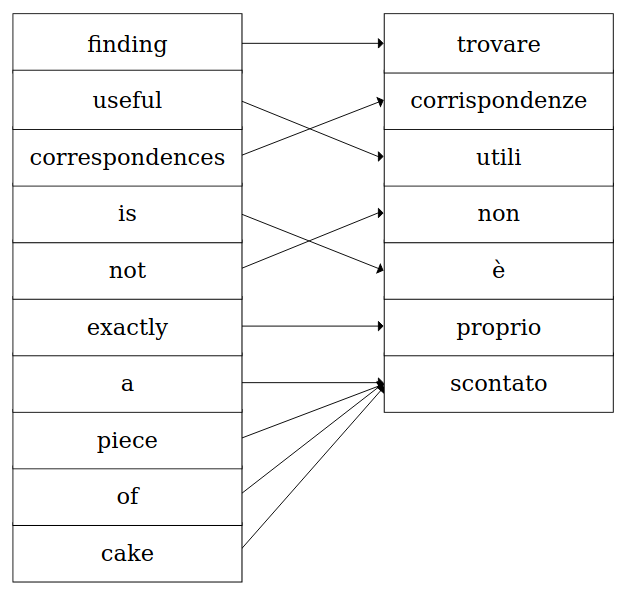
\includegraphics[width=.4\linewidth]{figure/alignment.png}
    \caption[An English sentence aligned with its Italian translation]{An English sentence aligned with its Italian translation. In this case, we are looking for the smallest possible alignments, but it is also possible to find correspondences at a higher level of abstractions, such as ``\textit{useful correspondences}'' and ``\textit{corrispondenze utili}'', which puts two noun phrases in relation with each other.} \label{cake}
\end{figure}

In cases like this, a syntactical comparison between the two sentences can help, if not to extract meaningful correspondences only, which would be the case in the example above, where the complement of the copula ''\textit{is}'' (resp. ``\textit{è}'') is a multiword expression in English and a one-word in Italian, at least to obtain a series of alignments at all levels of abstraction from which to select the most relevant at a later stage\footnote{An example of a more difficult case could be the alternative translation ``Trovare corrispondenze utili non è proprio \textit{un gioco da ragazzi}'', roughly corresponding to ``\textit{a child's play}'' (literally ``\textit{a game (played) by children}''). In this case, trying to align the sentence based on a syntactical comparison would yield both ``\textit{piece of cake}''-``\textit{gioco da ragazzi}'' and the more questionable correspondences ``\textit{piece}''-``\textit{gioco}'' and ``\textit{of cake}-``\textit{da ragazzi}''.}. 
The idea is that, in rule-based MT, using aligned phrases (as opposed to aligned words) is often useful for translating idiomatic expressions correctly and, in general, beneficial in terms of fluency of the output sentences.\smallskip
 
Furthermore, taking syntax into account allows to easily deal with non-contiguous multiword expressions, another situation which is challenging to deal with by means of traditional statistical approaches. For instance, if we consider the sentence ``\textit{Without any linguistic knowledge, it is definitely hard}'' and its Italian translation ``\textit{Senza conoscenze linguistiche, è decisamente arduo}'', a syntactical analysis would make it possible to extract the correspondence ``\textit{is hard}''-``\textit{è arduo}'', even if in both cases the copula and its complement are separated by an adverb. \smallskip

Last but not least, a syntax-based approach can produce correspondences between grammatical objects, as opposed to pairs of strings. Alignments of this kind are valuable, as they can more easily be utilized in rule-based MT systems. \smallskip

% contribution (+ sw deliverables w technologies involved)
With this thesis, we propose a syntax-based approach to both of the above mentioned variants of CA - concept extraction and concept propagation - composed of a neural Universal Dependencies (UD) parser and a rule-based alignment module.
We put our system to the test by integrating it in a prototype domain-specific MT system based on Grammatical Framework (GF).

\section*{Structure of the thesis}
This work is structured as follows. 
Chapter \ref{ch2} gives a few basic definitions, including a more rigorous one of CA itself, as well as providing the necessary background and contextualizing our project by reviewing a few related works. 
Chapters \ref{ch3} and \ref{ch4} focus respectively on extraction and propagation, presenting both our approach to each task and the corresponding experimental results, while Chapter \ref{ch5} describes the experiment designed to produce evaluate how well our CA component performs in the context of MT. 
Finally, Chapter \ref{ch6} consists of a discussion of the overall results and proposes some ideas for future work.

% THEORY AND TECHNOLOGIES
% CREATED BY DAVID FRISK, 2016
\chapter{Theory and Technologies} \label{ch2} 
In this chapter, we first review the preliminary notions of Computational Linguistics relevant to this work. 
We then give a more rigorous definition of the problem at hand and present the basic idea behind our proposed automation approach, comparing it to the existing ones and mentioning the technologies involved.

\section{Preliminary notions}
This first section consists of an overview of the basic notions that are necessary for a full understanding of the approach we propose. 
First, we discuss the principle of compositionality. 
After that, we describe and compare the grammar formalisms involved in the project, focussing on the two playing the most prominent roles in this work and comparing them to other, related approaches.

\subsection{Semantic compositionality}
The principle of semantic compositionality states, in its most general form, that the meaning of a complex expression is determined solely by the meanings of its components and by the manner in which these components are combined \cite{frege}. \smallskip 

A useful variant of this formulation, which refers to natural languages in particular, is the following: \smallskip

\begin{definition} \label{sc}
For every complex expression $e$ in a language $L$, the meaning of $e$ in $L$ is determined by the structure of $e$ and the meanings of the constituents of $e$ in $L$.
\end{definition}
\smallskip

Questions of structure and constituency are settled by the syntax of $L$, while the meanings of simple expressions are given by the lexical semantics of $L$, meaning that syntax and lexical semantics, together, are sufficient to determine the entire semantics of $L$ \cite{frege}. \smallskip

According to this definition, then, if $L$ is compositional, the meaning of an expression $e$ in $L$ cannot depend directly on the context in which $S$ is used in or on the intentions of the speaker who uses it, even though it might be the case that the meanings of the constituents of $e$ depend on the context or on the speaker's intentions, thus making the sentence indirectly depend on them \cite{semcom2}. \smallskip

While many artificial languages, such as programming languages, are compositional by construction, the general validity of this principle for natural languages is, despite many arguments in favor, under debate. 
In this work, we make the assumption that compositionality also holds for natural languages, or at least that it is a useful notion applying to most natural language sentences\footnote{in Section \ref{evalign}, however, we will see that idiomatic expressions, often used as an arguments against compositionality, are also challenging to deal with in the context of grammar-based CA.}. \smallskip

In particular, we adapt the notion of semantic compositionality to translation. 
The intuitive idea is that the translation of a sentence is composed of translations of each part of the original one. Adjusting Definition \ref{sc}:

\begin{definition}
    For every complex expression $e$ in a source language $S$, the translation of $e$ in a target language $T$ is determined by the structure of $e$ and the translations of the constituents of $e$ in $T$.
\end{definition}

\subsection{Constituency grammars}
The idea of taking advantage of semantic compositionality is not new in the field of Computational Linguistics. 
Doing so traditionally involves using some kind of \textit{constituency grammar}. \smallskip

The notion of constituency or \textit{phrase structure} grammar, introduced by Noam Chomsky in \cite{chomsky}, is usually known to computer scientists due to the fact that a class of phrase structure grammars, namely that of \textit{Context-Free Grammars} (CFGs), that can be used to describe programming languages and plays an central role in compiler theory. 
As a consequence, we find giving a complete formal definition of the latter unnecessary and will restrict ourselves to an informal review of the aspects that are particularly relevant for the specific subject of this thesis. \smallskip

A constituency grammar consists essentially in a set of \textit{rewrite rules}, such as 

\begin{lstlisting}[frame=none]
    S -> NP VP,
\end{lstlisting}

which we can read as ``$S$ can be \textit{rewritten as} (or \textit{substituted with}) a $\mathit{NP}$ followed by a $\mathit{VP}$'', or as ``a sentence $S$ is constituted by a noun phrase $\mathit{NP}$ and a verb phrase $\mathit{VP}$''. \smallskip

\begin{figure}[h]
    \centering
    \begin{subfigure}{.35\textwidth}
      \centering
      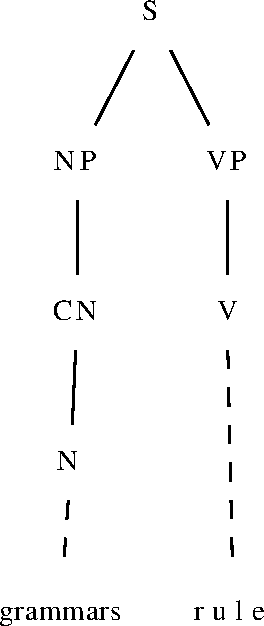
\includegraphics[width=.4\linewidth]{figure/parsetree.pdf}
    \end{subfigure}%
    \begin{subfigure}{.6\textwidth}
        \centering
        \begin{lstlisting}
            S -> NP VP
            NP -> CN
            VP -> V
            CN -> N
            N -> "grammars"
            V -> "rule"
        \end{lstlisting}
    \end{subfigure}
    \caption[Parse tree of the sentence ``\textit{grammars rule}'' and corresponding grammar fragment]{Parse tree of the simple sentence ``\textit{grammars rule}''. On the right, the fragment of the simple but linguistically informed grammar necessary to obtain such tree.}
    \label{pt}
\end{figure}

Replacing the term ``constituted'' with ``composed'' makes it easy to understand in which way phrase structure grammars are related to the aforementioned principle of compositionality. \smallskip

In the context of MT, the idea of exploiting the constituency relation and, as such, compositionality, was proposed by Curry in the early 1960s \cite{curry61} and first put in practice two decades later in the form of an experimental interlingual translation system, not coincidentally named Rosetta, which requires the definition of two distinct logically isomorphic \textit{Montague grammars}\footnote{Montague grammars are a semantics-oriented development of \textit{categorial grammars}, which are in turn a type of constituency grammars.} - one for the Source Language (SL), one for the Target Language (TL) - and constructs an intermediate representation based on such isomorphism \cite{rosetta}. \smallskip

\subsubsection{Synchronous grammars}
Among constituency grammars, other formalisms that have been employed in more recent MT systems are that of \textit{synchronous CFG}, originally developed for programming language compilation \cite{scfg} and adapted to natural language translation in several settings \cite{nlpscfg0,nlpscfg1,nlpscfg2,nlpscfg3}, and, later on, that of \textit{synchronous TAG} \cite{stag}, a variation of \textit{TAG} (Tree-Adjoining Grammar) \cite{tag}.
Both formalisms are meant to characterize correspondences between languages by having as their elements, instead of single rewrite rules, pairs of rules - one for the source and one for the target language. 
In a synchronous TAG, the constituents of a SL rule may be linked to their counterparts in the corresponding TL rule, and such links may be used to identify concepts in a syntax-based fashion. \smallskip

\subsubsection{Grammatical Framework} \label{gf}
% translation as compilation
As the repeated mention of programming language compilers in the above may suggest, it is possible to draw a very close parallel between compiler and MT pipelines. From this perspective, a natural language translation system can consist of: \smallskip

\begin{itemize}
    \item a \textit{frontend}, where the SL is analyzed or \textit{parsed} and whose output is an \textit{intermediate representation} most frequently in the form of an \textit{Abstract Syntax Tree} (AST)
    \item a \textit{backend}, where the AST is \textit{linearized} by means of application of a set of rules, a process usually referred to as \textit{code generation} in the context of programming languages and that we will refer to as \text{Target Language Generation} (TLG) or, when the context makes it clear that what the TL is, \textit{Natural Language Generation} (NLG). \smallskip
\end{itemize}
\begin{figure}[H]
    \centering
    
\includegraphics[width=.8\linewidth]{figure/compiler.png}
    \caption[Steps of programming language compilation and, in the case of GF, natural language translation]{Steps of programming language compilation and, in the case of GF, natural language translation. In compilation, the input is usually a high-level programming language and the output is machine code (or code in a lower-level language). In the case of MT, the input and the output are strings in two different natural languages.} \label{compilerd}
\end{figure}

% intro to GF
Grammatical Framework (GF), being a grammar formalism and programming language designed with this parallel in mind, goes a step further in the direction of synchronous CFGs and TAGs. 
It introduces in fact a clear distinction between the \textit{abstract syntax}, whose aim is to capture the syntactic structures all natural languages taken into account have in common, and the \textit{concrete syntaxes}, specific to each individual language, consisting in their linearization rules \cite{gf2004} \cite{gfbook}. 
This makes it possible to deal with multiple languages by writing only one grammar, whose components are an abstract syntax and several concrete syntaxes, providing a solid basis for a system able to translate between any pair of for which a concrete syntax is available, in any direction. \smallskip

% GF as an interlingua-based MT system
With respects to this, GF can be also seen as an \textit{interlingual} MT system where the intermediate representation or \textit{interlingua} is an AST. Interlingua-based systems have the advantage, in terms of efficiency, of making it unnecessary to build $n (n - 1)$ translation functions to cover all possible pairs of $n$ languages: having $2n$ is in general enough. In GF in particular, using a multilingual grammar makes it so that translation can be performed, for each pair of languages, in both directions, so that $n$ translation functions (or rahter $n$ concrete syntaxes and an abstract syntax) are already sufficient.\smallskip

% the RGL
An advantage of GF in particular, in addition, is the availability of a set of \textit{resource grammars} - the Resource Grammar Library (RGL) - for a variety of languages. A resource grammar is essentially a grammar that captures only the syntactic and morphological structures of a language, i.e. a grammar in the traditional sense of the term, and that can be easily extended to construct what is usually referred to as an \textit{application grammar}, i.e. a domain-specific grammar aiming to describe the language in a way that is not only syntactically correct, but also semantically accurate \cite{gfbook}. \smallskip

% GF and xMT
Extending the RGL in various ways, translation experiments with GF grammars have been conducted in the field of eXplainable Machine Translation (XMT), as the ASTs produced by SL analysis can serve both as to some extent automatically checkable certificates for the correctness of translation - by backlinearization to the SL - and as fully inspectable explanations aimed towards expert users \cite{rantaxmt}. \smallskip

% limitations
While the approach described above has proved successful for domain-specific translation, i.e. in cases where the natural languages in question can be reduced to \textit{Constrained Natural Languages} (CNLs), when it comes to open-domain translation, while target language generation remains effective, the results are negatively affected by the lack of robustness of the GF-based parsers available at the time of writing.

\subsection{Dependency grammars} \label{depg}
% DGs as opposed to PSGs
A class of grammar formalisms alternative to phrase structure, first proposed in \cite{dg}, is that of \textit{dependency grammars}, the main difference between the two being the relation they are based on. 
As opposed to constituency, \textit{dependency} is a word-to-word correspondence, meaning that words are simply put in relation with each other via directed links, called in fact \textit{dependencies}. 
Each dependency is, then, composed of two words: a \textit{head} and a \textit{dependent} that refers to it. For instance, if we try to look at syntactic dependencies in the sentence ``\textit{grammars rule}'', we could identify the verb ``\textit{rule}'' as the head and the noun ``\textit{grammars}'', its subject, as its dependent. \smallskip 

% pros
Intuitively, this means that dependency trees are simpler than their phrase structure counterparts. This makes them an easier target for the frontend, possibly ML-based, of a MT system such as the one outlined in the above. 
Existing \textit{dependency parsers}, such as UDPipe \cite{udpipe1} and the Standford parser \cite{standford}, are often - but not always \cite{rasp} - neural pipelines trained on dependency treebanks, significantly more robust than their phrase structure counterparts. 

% cons
On the other hand, there is currently no effective way to use these trees as a starting point for NLG: dependency grammars are an effective way to describe language, but, unlike phrase-structure grammars, they are not \textit{generative},\footnote{that does not mean, however, that dependency grammars have not been made use of in MT research, in conjunction with statistical techniques, in order to better capture grammatical generalizations \cite{treelet}.}. \smallskip

One idea is, then, to develop a hybrid system where the frontend is a dependency parser and the backend a grammaticality-preserving GF-based target language generation module. 
This work goes in this direction, and the connecting link between these two seemingly incompatible stages of the pipeline is, as we will elaborate on in Section \ref{ourapproach}, a CA component able to identify matching dependency trees and generate the corresponding GF concrete and abstract syntax functions: concepts.

While there are several different dependency-based frameworks, the following section focuses on the one we find most well suited to this purpose, \textit{Universal Dependencies}. 

\subsubsection{Universal Dependencies} \label{ud} 
Universal Dependencies (UD) is a framework for cross-linguistically consistent grammatical annotation. 
The UD project aims at developing parallel treebanks for many languages in order to support, among other things, the development of multilingual dependency parsers, such as the aforementioned UDPipe \cite{udpipe1}. 
In order to do so, it specifies an annotation scheme and a standard format for dependency trees consisting in an evolution of (universal) Stanford dependencies \cite{st1, st2}, Google universal part-of-speech tags \cite{upos}, and the Interset interlingua for morphosyntactic tagsets \cite{tagconv}. 
The basic idea behind such standard is to provide a set of Part-Of-Speech (POS) tags, dependency relations and annotation guidelines as language-agnostic as possible - so to facilitate its application in multilingual settings - while allowing language-specific extensions whenever necessary. \smallskip

In the following, we give a quick overview of the standard format UD uses to store dependency trees and of the aspects of the annotation scheme that are most relevant to the task at hand. 
Appendix \ref{a} provides a more comprehensive, but not completely exhaustive, description of all the POS tags and dependency labels mentioned in the examples appearing in this work based on that in \cite{compsyn}. 
The reader interested in a full specification of the UD annotation scheme may refer to the official UD documentation\footnote{available at \url{universaldependencies.org}.}. 

\paragraph{The CoNLL-U format} \label{conll}
The standard plain text format for dependency trees, CoNLL-U, is an extension of CoNNL-X \cite{conllx} which may contain \textit{comment lines}, starting with \texttt{\#}, \textit{blank lines} marking sentence boundaries and \textit{word lines} containing the annotation of a single token (generally a word, with some exceptions\footnote{examples of such exceptions are Italian contractions such as ``\textit{dello}'', which is generally divided into ``\textit{del}'' + ``\textit{lo}''.} in 10 tab-separated fields: \smallskip

\begin{enumerate}
    \item \texttt{ID}: integer\footnote{again, there are exceptions: in the case of Italian contractions and other multiword tokens, ranges may be used. Furthermore, empty nodes are characterized by decimal numbers between 0 and 1.} representing the position of the word in the sentence, starting from 1
    \item \texttt{FORM}: inflected from of the word
    \item \texttt{LEMMA}: lemmatized form of the word
    \item \texttt{UPOS}: universal POS tag
    \item \texttt{XPOS}: language-specific POS tag (optional)
    \item \texttt{FEATS}: list of (universal or language-specific) morphological features (optional)
    \item \texttt{HEAD}: head of the current word, i.e. either the value of the \texttt{ID} of another word in the same sentence or 0 in case the word at hand is a \texttt{root}
    \item \texttt{DEPREL}: universal dependency relation to the \texttt{HEAD} (\texttt{root} in case the word at hand is itself the \texttt{root})
    \item \texttt{DEPS}: enhanced dependency graph in the form of a list of \texttt{HEAD}-\texttt{DEPREL} pairs (optional)
    \item \texttt{MISC}: any other annotation (optional)
\end{enumerate} \smallskip

\begin{figure}[h]
    \centering
    \begin{subfigure}{.55\textwidth}
      \centering
      \footnotesize
        \begin{verbatim}
1	this	this	PRON	_	_	5	nsubj	_	_
2	is	be	AUX	_	_	5	cop	_	_
3	a	a	DET	_	_	5	det	_	_
4	dependency	dependency	NOUN	_	_	5	compound	_	_
5	tree	tree	NOUN	_	_	0	root	_	_
        \end{verbatim}
    \end{subfigure}%
    \begin{subfigure}{.45\textwidth}
        \centering
        \footnotesize
        \setlength{\unitlength}{0.21mm}
        \begin{picture}(371.0,130.0)
            \put(0.0,0.0){this}
            \put(46.0,0.0){is}
            \put(83.0,0.0){a}
            \put(120.0,0.0){dependency}
            \put(220.0,0.0){tree}
            \put(0.0,15.0){{\tiny PRON}}
            \put(46.0,15.0){{\tiny AUX}}
            \put(83.0,15.0){{\tiny DET}}
            \put(120.0,15.0){{\tiny NOUN}}
            \put(220.0,15.0){{\tiny NOUN}}
            \put(120.0,30.0){\oval(218.63636363636363,133.33333333333334)[t]}
            \put(10.681818181818187,35.0){\vector(0,-1){5.0}}
            \put(105.0,99.66666666666667){{\tiny nsubj}}
            \put(143.0,30.0){\oval(172.27586206896552,100.0)[t]}
            \put(56.86206896551724,35.0){\vector(0,-1){5.0}}
            \put(128.0,83.0){{\tiny cop}}
            \put(161.5,30.0){\oval(134.8102189781022,66.66666666666667)[t]}
            \put(94.0948905109489,35.0){\vector(0,-1){5.0}}
            \put(146.5,66.33333333333334){{\tiny det}}
            \put(180.0,30.0){\oval(97.0,33.333333333333336)[t]}
            \put(131.5,35.0){\vector(0,-1){5.0}}
            \put(165.0,49.66666666666667){{\tiny compound}}
            \put(235.0,130.0){\vector(0,-1){100.0}}
            \put(240.0,120.0){{\tiny root}}
        \end{picture}
    \end{subfigure}
    \caption[A dependency tree in CoNNL-U format alongside its graphical representation]{A dependency tree in CoNNL-U format alongside its graphical representation. Optional fields in the CoNLL-U file are left blank.}
    \label{deptree}
\end{figure}

\paragraph{Universal POS tags} \label{upos}
Universal POS tags mark the core part-of-speech categories, such as nouns, verbs, pronouns and determiners. \smallskip

An important distinction we can make based on POS tags is, as we will see in Section \ref{criteria}, that between \textit{content} and \textit{function} words.
\textit{Content} or \textit{open class} words are words with a lexical meaning (nouns, lexical verbs, adjectives, adverbs and interjections).
\textit{Function} words, like pronouns and determiners, only have a grammatical meaning. Since they do not readily accept new members\footnote{one exception is the recent introduction of the gender-neutral pronoun ``\textit{hen}'' in Swedish.}, they are often referred to also as \textit{closed class} words. \smallskip

While the majority of Universal POS tags correspond to the grammatical categories of traditional grammars, the UD annotation scheme does have its peculiarities. 
Most importantly for the following discussion, verbs are divided into lexical verbs, tagged \texttt{VERB}, and auxiliaries, tagged \texttt{AUX}, thus providing an easy way to distinguish between content verbs and function verbs. 
A more systematic description of \texttt{UPOS} tags is given in \ref{a_pos}.

\paragraph{Universal dependency relations}
%subtypes
Universal dependency relations, largely based on \cite{st2}, represent, as mentioned in the above, syntactic dependencies between individual pairs of words occurring in the same sentence. 
In particular, according to the CoNLL-U standard (cf. Section \ref{conll}), each word is assigned a \textit{dependency label} indicating in which way it is liked to its \texttt{HEAD}. \smallskip 

In this sense, the only exceptional case, which will be the starting point for our short overview of dependency relations, is that of the \texttt{root} label, generally assigned to the main verb of a sentence, ignoring any auxiliaries. 
For instance, ``\textit{smoked}'' is the root of the sentence \smallskip

\begin{example} \label{katia1}
    ``Katia has just \underline{smoked} a cigarette''
\end{example} \smallskip

In cases such as the following, where the main verb is a copula, the root is its complement and the verb is linked to it with the label \texttt{cop}. \smallskip

\begin{example} \label{katia2}
    ``Katia is a \underline{psychologist}''
\end{example} \smallskip

 If a sentence contains is no verbs at all, there is no fixed rule excepts that, in order to avoid unnecessary discrepancies between languages, the root should be a content word. \smallskip

\begin{figure}[h]
   \centering
   \scriptsize
   \begin{subfigure}{.5\textwidth}
        \centering
        \setlength{\unitlength}{0.24mm}
        \begin{picture}(380.0,110.0)
            \put(0.0,0.0){Katia}
            \put(55.0,0.0){has}
            \put(92.0,0.0){just}
            \put(138.0,0.0){smoked}
            \put(202.0,0.0){a}
            \put(239.0,0.0){cigarette}
            \put(0.0,15.0){{\tiny PROPN}}
            \put(55.0,15.0){{\tiny AUX}}
            \put(92.0,15.0){{\tiny ADV}}
            \put(138.0,15.0){{\tiny VERB}}
            \put(202.0,15.0){{\tiny DET}}
            \put(239.0,15.0){{\tiny NOUN}}
            \put(79.0,30.0){\oval(135.82608695652175,100.0)[t]}
            \put(11.086956521739125,35.0){\vector(0,-1){5.0}}
            \put(64.0,83.0){{\tiny nsubj}}
            \put(106.5,30.0){\oval(79.3855421686747,66.66666666666667)[t]}
            \put(66.80722891566265,35.0){\vector(0,-1){5.0}}
            \put(91.5,66.33333333333334){{\tiny aux}}
            \put(125.0,30.0){\oval(39.47826086956522,33.333333333333336)[t]}
            \put(105.26086956521739,35.0){\vector(0,-1){5.0}}
            \put(110.0,49.66666666666667){{\tiny advmod}}
            \put(230.5,30.0){\oval(28.89189189189189,33.333333333333336)[t]}
            \put(216.05405405405406,35.0){\vector(0,-1){5.0}}
            \put(215.5,49.66666666666667){{\tiny det}}
            \put(208.5,30.0){\oval(98.02970297029702,66.66666666666667)[t]}
            \put(257.5148514851485,35.0){\vector(0,-1){5.0}}
            \put(193.5,66.33333333333334){{\tiny obj}}
            \put(153.0,110.0){\vector(0,-1){80.0}}
            \put(158.0,100.0){{\tiny root}}
          \end{picture}
   \end{subfigure}%
   \begin{subfigure}{.5\textwidth}
        \centering
        \setlength{\unitlength}{0.20mm}
        \begin{picture}(474.0,150.0)
            \put(0.0,0.0){Katia}
            \put(55.0,0.0){has}
            \put(92.0,0.0){worked}
            \put(156.0,0.0){in}
            \put(193.0,0.0){a}
            \put(230.0,0.0){big}
            \put(267.0,0.0){school}
            \put(331.0,0.0){library}
            \put(0.0,15.0){{\tiny PROPN}}
            \put(55.0,15.0){{\tiny AUX}}
            \put(92.0,15.0){{\tiny VERB}}
            \put(156.0,15.0){{\tiny ADP}}
            \put(193.0,15.0){{\tiny DET}}
            \put(230.0,15.0){{\tiny ADJ}}
            \put(267.0,15.0){{\tiny NOUN}}
            \put(331.0,15.0){{\tiny NOUN}}
            \put(56.0,30.0){\oval(88.73913043478261,66.66666666666667)[t]}
            \put(11.630434782608695,35.0){\vector(0,-1){5.0}}
            \put(41.0,66.33333333333334){{\tiny nsubj}}
            \put(83.5,30.0){\oval(28.89189189189189,33.333333333333336)[t]}
            \put(69.05405405405405,35.0){\vector(0,-1){5.0}}
            \put(68.5,49.66666666666667){{\tiny aux}}
            \put(253.5,30.0){\oval(173.28571428571428,133.33333333333334)[t]}
            \put(166.85714285714286,35.0){\vector(0,-1){5.0}}
            \put(238.5,99.66666666666667){{\tiny case}}
            \put(272.0,30.0){\oval(135.82608695652175,100.0)[t]}
            \put(204.08695652173913,35.0){\vector(0,-1){5.0}}
            \put(257.0,83.0){{\tiny det}}
            \put(290.5,30.0){\oval(98.02970297029702,66.66666666666667)[t]}
            \put(241.4851485148515,35.0){\vector(0,-1){5.0}}
            \put(275.5,66.33333333333334){{\tiny amod}}
            \put(309.0,30.0){\oval(59.3125,33.333333333333336)[t]}
            \put(279.34375,35.0){\vector(0,-1){5.0}}
            \put(294.0,49.66666666666667){{\tiny compound}}
            \put(231.5,30.0){\oval(237.744769874477,166.66666666666666)[t]}
            \put(350.3723849372385,35.0){\vector(0,-1){5.0}}
            \put(216.5,116.33333333333333){{\tiny obl}}
            \put(107.0,150.0){\vector(0,-1){120.0}}
            \put(112.0,140.0){{\tiny root}}
          \end{picture}
   \end{subfigure}
   \begin{subfigure}{.4\textwidth}
        \centering
        \setlength{\unitlength}{0.2mm}
        \begin{picture}(277.0,110.0)
            \put(0.0,0.0){Katia}
            \put(55.0,0.0){is}
            \put(92.0,0.0){a}
            \put(129.0,0.0){psychologist}
            \put(0.0,15.0){{\tiny PROPN}}
            \put(55.0,15.0){{\tiny AUX}}
            \put(92.0,15.0){{\tiny DET}}
            \put(129.0,15.0){{\tiny NOUN}}
            \put(74.5,30.0){\oval(126.67441860465117,100.0)[t]}
            \put(11.162790697674417,35.0){\vector(0,-1){5.0}}
            \put(59.5,83.0){{\tiny nsubj}}
            \put(102.0,30.0){\oval(69.94594594594595,66.66666666666667)[t]}
            \put(67.02702702702703,35.0){\vector(0,-1){5.0}}
            \put(87.0,66.33333333333334){{\tiny cop}}
            \put(120.5,30.0){\oval(28.89189189189189,33.333333333333336)[t]}
            \put(106.05405405405405,35.0){\vector(0,-1){5.0}}
            \put(105.5,49.66666666666667){{\tiny det}}
            \put(144.0,110.0){\vector(0,-1){80.0}}
            \put(149.0,100.0){{\tiny root}}
          \end{picture}
   \end{subfigure}%
   \begin{subfigure}{.6\textwidth}
        \centering
        \setlength{\unitlength}{0.2mm}
        \begin{picture}(530.0,110.0)
            \put(0.0,0.0){Katia}
            \put(55.0,0.0){showed}
            \put(119.0,0.0){me}
            \put(165.0,0.0){a}
            \put(202.0,0.0){book}
            \put(248.0,0.0){about}
            \put(303.0,0.0){the}
            \put(340.0,0.0){Stone}
            \put(395.0,0.0){Age}
            \put(0.0,15.0){{\tiny PROPN}}
            \put(55.0,15.0){{\tiny VERB}}
            \put(119.0,15.0){{\tiny PRON}}
            \put(165.0,15.0){{\tiny DET}}
            \put(202.0,15.0){{\tiny NOUN}}
            \put(248.0,15.0){{\tiny ADP}}
            \put(303.0,15.0){{\tiny DET}}
            \put(340.0,15.0){{\tiny PROPN}}
            \put(395.0,15.0){{\tiny PROPN}}
            \put(37.5,30.0){\oval(49.54545454545455,33.333333333333336)[t]}
            \put(12.727272727272727,35.0){\vector(0,-1){5.0}}
            \put(22.5,49.66666666666667){{\tiny nsubj}}
            \put(107.0,30.0){\oval(59.3125,33.333333333333336)[t]}
            \put(136.65625,35.0){\vector(0,-1){5.0}}
            \put(92.0,49.66666666666667){{\tiny iobj}}
            \put(193.5,30.0){\oval(28.89189189189189,33.333333333333336)[t]}
            \put(179.05405405405406,35.0){\vector(0,-1){5.0}}
            \put(178.5,49.66666666666667){{\tiny det}}
            \put(148.5,30.0){\oval(144.9591836734694,66.66666666666667)[t]}
            \put(220.9795918367347,35.0){\vector(0,-1){5.0}}
            \put(133.5,66.33333333333334){{\tiny obj}}
            \put(304.0,30.0){\oval(88.73913043478261,66.66666666666667)[t]}
            \put(259.6304347826087,35.0){\vector(0,-1){5.0}}
            \put(289.0,66.33333333333334){{\tiny case}}
            \put(331.5,30.0){\oval(28.89189189189189,33.333333333333336)[t]}
            \put(317.05405405405406,35.0){\vector(0,-1){5.0}}
            \put(316.5,49.66666666666667){{\tiny det}}
            \put(217.5,30.0){\oval(283.94736842105266,100.0)[t]}
            \put(359.47368421052636,35.0){\vector(0,-1){5.0}}
            \put(202.5,83.0){{\tiny obl}}
            \put(387.5,30.0){\oval(49.54545454545455,33.333333333333336)[t]}
            \put(412.27272727272725,35.0){\vector(0,-1){5.0}}
            \put(372.5,49.66666666666667){{\tiny flat}}
            \put(70.0,110.0){\vector(0,-1){80.0}}
            \put(75.0,100.0){{\tiny root}}
          \end{picture}
    \end{subfigure}
      
   \caption[UD trees showing the common dependency relations that are discussed in Chapter \ref{ch3}]{UD trees showing the common dependency relations that are discussed in Chapter \ref{ch3}. The three on the left correspond to examples \ref{katia1} and \ref{katia2}.}
    \label{katia}
\end{figure}

Other dependency labels commonly found in simple clauses and that will be dwelt on in Chapter \ref{ch3}, all exemplified in Figure \ref{katia}, are: \smallskip
\begin{itemize}
    \item \texttt{nsubj}, marking the link between a noun, proper noun, pronoun or numeral to the \texttt{root} of a sentence or, more in general, to the head of a clause
    \item \texttt{aux}, marking auxiliary verbs other than the copula
    \item \texttt{obj}, \texttt{iobj} and \texttt{obl} marking the link between a verb and its object, indirect object and other complements respectively
    \item \texttt{advmod}, \texttt{amod}, \texttt{nummod} and \texttt{nmod}, marking links between modifiers and the nouns or verbs they refer to
    \item \texttt{flat}, indicating a flat multiword expression, and \texttt{compound}, appearing in compound nouns whenever they are written as two or more separate words.
\end{itemize} \smallskip

A more detailed description of all the UD labels mentioned in this work is given in \ref{a_lab}. 
However, because the topic will arise in Chapter \ref{ch3}, it is also worth mentioning that CoNNL-U trees can present UD labels followed by a \textit{subtype}, separated by the label itself by a semicolon and used to indicate grammatical relations that are specific to one language or a small group of related languages. A subtype that is commonly used in English is, for instance, \texttt{pass}, added to both the (clausal or nominal) syntactic subject and \texttt{aux} of a sentence in passive voice.

\begin{figure}[h]
    \centering
    \begin{subfigure}{.5\textwidth}
        \centering
        \setlength{\unitlength}{0.25mm}
\begin{picture}(259.0,90.0)
  \put(0.0,0.0){Katia}
  \put(55.0,0.0){reads}
  \put(110.0,0.0){a}
  \put(147.0,0.0){magazine}
  \put(0.0,15.0){{\tiny PROPN}}
  \put(55.0,15.0){{\tiny VERB}}
  \put(110.0,15.0){{\tiny DET}}
  \put(147.0,15.0){{\tiny NOUN}}
  \put(37.5,30.0){\oval(49.54545454545455,33.333333333333336)[t]}
  \put(12.727272727272727,35.0){\vector(0,-1){5.0}}
  \put(22.5,49.66666666666667){{\tiny nsubj}}
  \put(138.5,30.0){\oval(28.89189189189189,33.333333333333336)[t]}
  \put(124.05405405405405,35.0){\vector(0,-1){5.0}}
  \put(123.5,49.66666666666667){{\tiny det}}
  \put(121.0,30.0){\oval(88.73913043478261,66.66666666666667)[t]}
  \put(165.3695652173913,35.0){\vector(0,-1){5.0}}
  \put(106.0,66.33333333333334){{\tiny obj}}
  \put(70.0,90.0){\vector(0,-1){60.0}}
  \put(75.0,80.0){{\tiny root}}
\end{picture}
    \end{subfigure}%
    \begin{subfigure}{.5\textwidth}
        \centering
        \setlength{\unitlength}{0.25mm}
        \begin{picture}(344.0,90.0)
            \put(0.0,0.0){A}
            \put(37.0,0.0){magazine}
            \put(119.0,0.0){is}
            \put(156.0,0.0){read}
            \put(202.0,0.0){by}
            \put(239.0,0.0){Katia}
            \put(0.0,15.0){{\tiny DET}}
            \put(37.0,15.0){{\tiny NOUN}}
            \put(119.0,15.0){{\tiny AUX}}
            \put(156.0,15.0){{\tiny VERB}}
            \put(202.0,15.0){{\tiny ADP}}
            \put(239.0,15.0){{\tiny PROPN}}
            \put(28.5,30.0){\oval(28.89189189189189,33.333333333333336)[t]}
            \put(14.054054054054054,35.0){\vector(0,-1){5.0}}
            \put(13.5,49.66666666666667){{\tiny det}}
            \put(106.5,30.0){\oval(116.47899159663865,66.66666666666667)[t]}
            \put(48.260504201680675,35.0){\vector(0,-1){5.0}}
            \put(91.5,66.33333333333334){{\tiny nsubj:pass}}
            \put(147.5,30.0){\oval(28.89189189189189,33.333333333333336)[t]}
            \put(133.05405405405406,35.0){\vector(0,-1){5.0}}
            \put(132.5,49.66666666666667){{\tiny aux:pass}}
            \put(230.5,30.0){\oval(28.89189189189189,33.333333333333336)[t]}
            \put(216.05405405405406,35.0){\vector(0,-1){5.0}}
            \put(215.5,49.66666666666667){{\tiny case}}
            \put(217.5,30.0){\oval(79.3855421686747,66.66666666666667)[t]}
            \put(257.1927710843373,35.0){\vector(0,-1){5.0}}
            \put(202.5,66.33333333333334){{\tiny obl}}
            \put(171.0,90.0){\vector(0,-1){60.0}}
            \put(176.0,80.0){{\tiny root}}
          \end{picture}
    \end{subfigure}
    \caption[The UD trees of an example active sentence and its passive counterpart]{The UD trees of an example active sentence and its passive counterpart.}
    \label{actpass}
\end{figure}

\paragraph{Relation to GF} \label{udrelgf}
The complementarity of constituency and dependency grammars and the multilingual nature of UD make it interesting to use in conjunction with GF, and experiments aimed at exploiting their similarities have already been performed \cite{gfud, udgf}. 
In the case of hybrid MT pipelines as the one sketched in Section \ref{depg}, UD trees need to be at some point converted into GF ASTs, albeit with the disadvantage that, unlike its reverse, the UD-to-GF conversion is a non-deterministic search problem.
An algorithm for conversion in this direction is presented in \cite{udgf}, where \texttt{gf-ud}, a program for converting GF ASTs into UD trees initially presented in \cite{gfud}, is extended to also be able to do the reverse. 

\begin{figure}[h]
    \centering
    \begin{subfigure}{.7\textwidth}
        \centering
        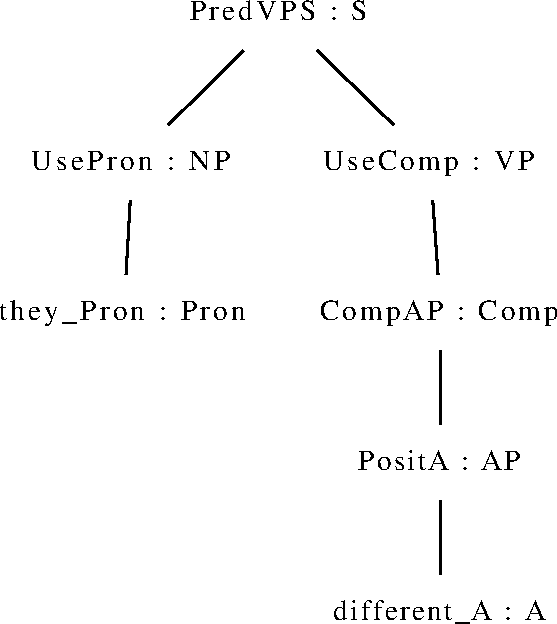
\includegraphics[width=.4\linewidth]{figure/different.pdf}
    \end{subfigure}%
    \begin{subfigure}{.3\textwidth}
        \centering
        \setlength{\unitlength}{0.25mm}
        \begin{picture}(194.0,90.0)
          \put(0.0,0.0){they}
          \put(46.0,0.0){are}
          \put(83.0,0.0){different}
          \put(0.0,15.0){{\tiny PRON}}
          \put(46.0,15.0){{\tiny AUX}}
          \put(83.0,15.0){{\tiny ADJ}}
          \put(51.5,30.0){\oval(79.3855421686747,66.66666666666667)[t]}
          \put(11.807228915662648,35.0){\vector(0,-1){5.0}}
          \put(36.5,66.33333333333334){{\tiny nsubj}}
          \put(74.5,30.0){\oval(28.89189189189189,33.333333333333336)[t]}
          \put(60.054054054054056,35.0){\vector(0,-1){5.0}}
          \put(59.5,49.66666666666667){{\tiny cop}}
          \put(98.0,90.0){\vector(0,-1){60.0}}
          \put(103.0,80.0){{\tiny root}}
        \end{picture}
    \end{subfigure}
    \caption[A GF AST and its UD counterpart]{A GF AST and its UD counterpart. Note how the copula is implicit in the GF AST and subordinate to its complement in UD.}
    \label{parsetree}
\end{figure}


\section{Concept Alignment}
In this section, we aim to give an exhaustive description of CA and of the subtasks it consists of. In order to do that, we deem it necessary to start by giving a definition of what we commonly refer to as \textit{concepts}. 

\subsection{Concepts} \label{concepts}
Intuitively, concepts are the components of meaning, and therefore, in a multilingual context, the units of translation. 
If we assume the principle of compositionality to be valid and apply it to translation, these meaning components are the common denominator between an expression in the source language and its translation, which can be generated using them as the starting point. \smallskip

From the compiler-like perspective described in Section \ref{gf}, this means that concepts are what the abstract syntax should represent, i.e. that they \textit{are} the ``interlingua'' of the MT system. 
This raises the question of how to obtain the abstract syntax needed for GF-based MT starting from a corpus of parallel texts, and it is at this point that language comparison and, as such, CA, come into play.

\subsection{Alignments} \label{aligns}
In terms of parallel text analysis, an \textit{alignment} consists in a pair of semantically equivalent (i.e., in this context, sharing the same abstract syntax) concrete expressions, one in the source and one in the target language. 
Even though, unless otherwise specified, we will keep referring to \textit{language pairs}, with a source and a target language, it is easy to see how this can be generalized to a more-than-bilingual, multidirectional definition.
The pair just mentioned simply becomes a tuple of equivalent expressions in different languages. Formally, \smallskip

\begin{definition} \label{algndef}
    An $n$-lingual \textit{alignment} is an $n$-uple $\langle e_1,...,e_n \rangle$ of semantically equivalent expressions, where each expressions $e_i$ is in a different language $L_i$.
\end{definition} \smallskip

While this general definition does not specify it, expressions are not necessarily represented as strings, but can rather be defined as tree-like structures, and in the present case as dependency trees that can later be replaced by GF ASTs. Matching ASTs can finally be used to generate the rules of a multilingual GF grammar, as we will discuss in Chapter \ref{ch5}. \smallskip

As mentioned in the introduction, the task of aligning concepts comes in two variants:
\begin{enumerate}
    \item \textbf{\textit{Concept Extraction}} (CE), which consists in identifying new concepts via linguistic comparison and whose output is a set of bilingual alignments
    \item \textbf{\textit{Concept Propagation}} (CP), i.e. the task of finding the concrete expressions corresponding to a set of known concepts in a particular language. Here, by concepts we do not mean necessarily ASTs, as a suitable approach is to propagate UD tree alignments before obtaining the corresponding abstract representation.
\end{enumerate} \smallskip

If, as in the case of this project, the aim is to develop a multilingual MT system, these two tasks can be seen as two potentially subsequent steps. A first objective, in fact, can be to extract a set of concepts by comparing two translations of the same text. Once these concepts are in adequate number and of sufficient quality, it becomes possible to provide support for additional languages by simply looking for the concrete expressions that, in the new language, correspond to each of the previously gathered concepts. In other situations, clearly, CE alone can be enough or, if a set of concepts is already known, CP can be applied independently from CE to find their equivalents in a new language.

\subsection{Approaches to automation} 
Some form of manual, semi- or fully automated CA is in a sense at the heart of all traditional, even very early, MT systems. 
In the following section, we review some standard approaches. After discussing their limitations, we conclude the chapter with an overview of the grammar-based approach proposed in this thesis.

\subsubsection{Existing methods} \label{statmt}  
In the simplest case, \textit{word alignment} consists in finding pairs of individual words that translate to each other and store them in a dictionary. 
The standard automatic approaches to this task are statistical, and among them the five IBM Models \cite{ibm} and their numerous variations stand out. 
The IBM Models are a sequence of increasingly complex alignment models \cite{bitext}: \smallskip

\begin{itemize}
    \item Model 1 is based exclusively on lexical translation probabilities
    \item Model 2 takes word order (i.e. the absolute word positions) into account 
    \item Model 3 takes even a \textit{fertility} parameter into account (fertility being the number of target words that can be generated from a given source word)
    \item Models 4 and 5 take the \textit{context} (i.e. the relative position of the words) in which each word occurs into account in a broader sense
\end{itemize}

The GIZA++ toolkit \cite{gizapp}, an open source implementation of the IBM models based on the initial GIZA package \cite{giza}, is widely used, for instance in SMT systems such as Moses \cite{moses}. \smallskip

As mentioned in the introduction, however, alignment can be performed at different levels of abstraction: to bring this to the extreme, there are contexts in which we might want to align full sentences, or even whole documents. While the latter two levels of abstraction are not necessarily relevant to MT, only aligning individual words is also, as discussed in the Introduction, not always the best option. For this reason, word alignment is often generalized to \textit{phrase alignment}. In systems like GIZA++, whose output is a list of pairs of word positions indicating which words in the SL string are to be aligned with which words in the TL string (commonly referred to as the \textit{pharaoh format}), extracting phrase alignments by combining the indices is realtively straightforward. \smallskip 

\begin{figure}[h]
    \centering
    \begin{subfigure}{.55\textwidth}
      \centering
      \footnotesize
      \begin{itemize}
          \item[SL] ``\textit{Word alignment with standard statistical tools}''
          \item[TL] ``\textit{Allineamento parola per parola con strumenti statistici standar}''
      \end{itemize}
    \end{subfigure}%
    \begin{subfigure}{.45\textwidth}
        \centering
        \footnotesize
        \setlength{\unitlength}{0.21mm}
        \begin{verbatim}
    0-1 0-2 0-3 1-0 2-4 3-7 4-6 5-5
        \end{verbatim}
    \end{subfigure}
    \footnotesize
    \smallskip
    \smallskip
    \begin{itemize}
        \item \texttt{0-1 0-2 0-3}: $\langle$\textit{``word'', ``parola per parola''}$\rangle$
        \item \texttt{1-0}: $\langle$\textit{``alignment'', ``allineamento''}$\rangle$
        \item \texttt{2-4}: $\langle$\textit{``with'', ``con''}$\rangle$
        \item \texttt{3-7}: $\langle$\textit{``standard'', ``standard''}$\rangle$
        \item \texttt{4-6}: $\langle$\textit{``statistical'', ``statistici''}$\rangle$
        \item \texttt{5-5}: $\langle$\textit{``tools'', ``strumenti''}$\rangle$
        \item \texttt{0-1 0-2 0-3 1-0}: $\langle$\textit{``word alignment'', ``allineamento parola per parola''}$\rangle$
        \item ...
    \end{itemize}
    ...
    \caption[The pharaoh format output of optimal word alignment on a pair of Italian-English sentences and some derived phrase alignments]{The pharaoh format output of optimal word alignment on a pair of Italian-English sentences and, below, some of the phrase alignments that can be derived from it.}
    \label{wordalgn}
\end{figure}

However, it must be noted that, in the context of statistical MT, the term ``phrase'' is not to be intended in its grammatical sense, but can refer to any sequence of - typically contiguous - words. 
In any case, both for word and phrase alignment, the relation that is established with these statistical methods is merely between strings in different languages: there is no intermediate representation capturing the concepts themselves. \smallskip

The parallel between MT and compiler pipelines proposed in Section \ref{gf} suggests instead that a more flexible approach, applicable at any level of abstraction, could be grammar-based. 
This is particularly useful in cases, not at all uncommon, where the minimal translation units are, in one or both the source and the target language, multiword - potentially discontinuous - expressions or even more complex constructions that phrase alignment is not able to handle. \smallskip 

Over time, various constituency grammar-based approaches have been proposed \cite{t2t1, t2t2}. 
These approaches, which make use of parallel treebanks, can be referred to as \textit{tree-to-tree alignment} methods \cite{bitext}. 
While theoretically appealing, however, their use in data-driven MT is limited, since they tend to suffer not only from the scarce availability of large-scale manually annotated corpora and the lack of robustness of the existing parsers, but also from the fact that, in general, the monolingual grammars used for parsing tend to be designed independently from each other, following different traditions, formalisms and linguistic theories \cite{nlphandbook}, thus making it often impossible to find a common representation describing a complete mapping from one tree to another \cite{bitext}.

\subsubsection{Our approach} \label{ourapproach}
Given that GF solves the latter problem, that it provides a good basis for NLG and that the intermediate representations it makes use of preserve all the syntactic information present in a sentence, the idea of trying to perform CA by comparing GF ASTs seems tempting. 
However, since ASTs need to be obtained from raw - or, at most, barely sentence-segmented - text, CA would suffer from the same problem that, as mentioned in in Section \ref{gf}, affects other tree-to-tree alignment methods and GF-based open-domain translation: the lack of a sufficiently robust analysis stage and, as a consequence, the inadequacy of the resulting parse trees. \smallskip

As anticipated throughout this chapter, we attempt to solve this problem by taking advantage of dependency parsing. 
In particular, UD is our formalism of choice since its focus on ``universality'' (i.e. on abstracting away from cross-lingual differences) makes it as interesting as GF itself when it comes to the possibility of establishing mappings between trees in different languages. 
Furthermore, when it comes to MT itself, using UD allows us to take advantage of the tools that have been developed to leverage its similarities with GF (cf. Section \ref{ud}), thus enabling GF target language generation. \smallskip

Concretely, this means that the system we propose requires the following elements, whose reciprocal relations are shown in Figure \ref{elems}: \smallskip

\begin{itemize}
    \item a UD parser
    \item an alignment module based on dependency tree comparison, which is the tangible output of this project and whose CE and CP components are described and evaluated in detail in Chapters \ref{ch3} and \ref{ch4} respectively
    \item a program, based on \texttt{gf-ud}, that converts the alignments into GF ASTs to then generate a domain-specific GF lexicon\footnote{CA is performed on UD trees, i.e. before conversion to GF, to reduce the possibility of errors. The reason is that, as mentioned in Section \ref{udrelgf}, in fact, such conversion is not obtained by means of a deterministic procedure and, as such, is not always guaranteed to be correct.}.
\end{itemize} \smallskip

The CE and CP modules are implemented as part of the project, while the UD parser and \texttt{gf-ud} are independently developed open source software, even though the latter, being currently under development was adapted and extended as part of the process. 
In addition, we provide a simple GF-based translation script to evaluate the performance of the CA module to the test.

\begin{figure}[h]
    \centering
    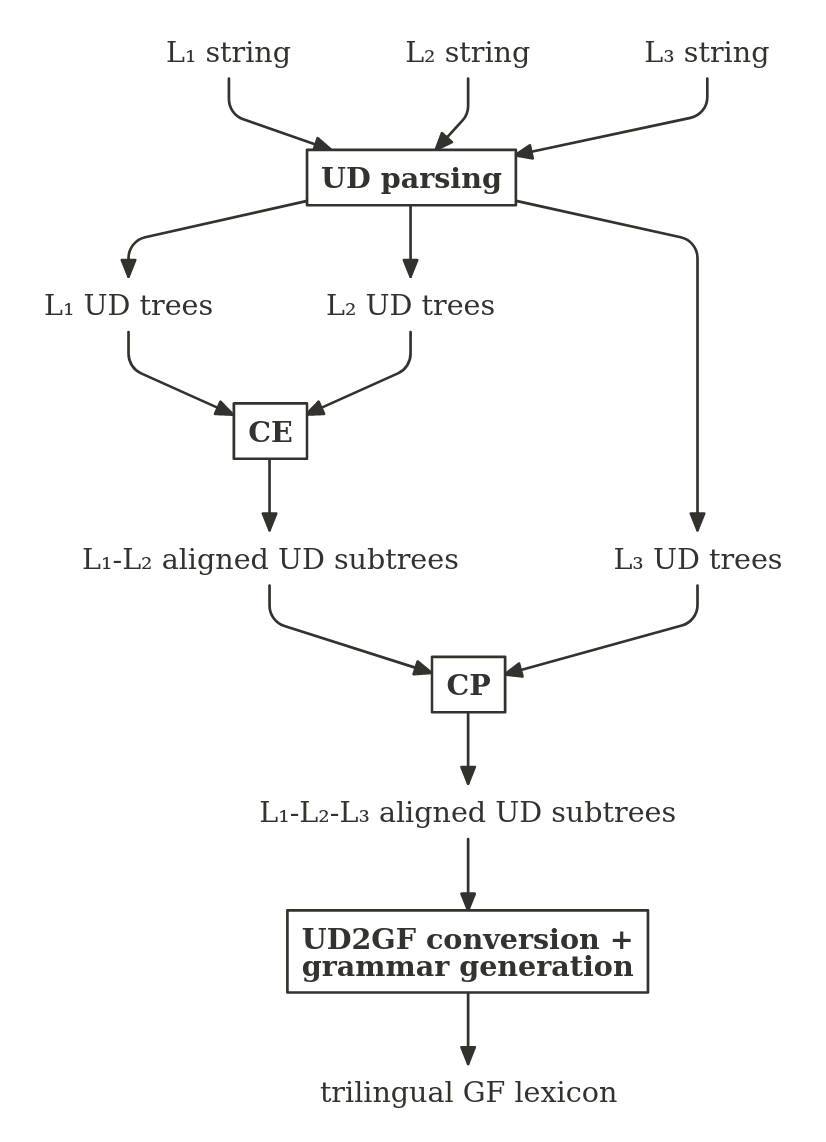
\includegraphics[width=.6\linewidth]{figure/elems.png}
    \caption[Relationship between the different components of the CA system]{Relationship between the different components of the system proposed in this work. The diagram shows the minimal, trilingual use case in which both CE and CP can be made use of.} \label{elems}
    \label{sys}
\end{figure}


% CONCEPT EXTRACTION
% CREATED BY DAVID FRISK, 2016
\chapter{Concept Extraction} \label{ch3} 
As mentioned in Section \ref{aligns}, extracting a set of concepts via linguistic comparison is the first and most important step of CA. This chapter describes our CE module, delineates our strategy to evaluate it independently from the other components of the system illustrated in Figure \ref{sys} and presents the results of such preliminary evaluation.

\section{Method and implementation} \label{ce}
For the reasons discussed in Section \ref{ourapproach}, our syntax-based approach to CE is based on comparing, instead on ASTs, dependency trees, and UD trees in particular.
The task of dealing with UD trees is facilitated by the existence of a series of Haskell modules written in the context of the development of the aforementioned \texttt{gf-ud} and of some preliminary unpublished CA experiments\footnote{Aarne Ranta and Prasanth Kolachina, code available at \url{github.com/aarneranta/concept-alignment/tree/master/old_ca_versions/v1}}. \smallskip

In this context, as shown in Figure \ref{types}, dependency trees are represented as rose trees, i.e. tree data structures with an unbounded, variable number of branches per node.

\begin{figure}[H] 
  \centering
  \lstinputlisting{pseudocode/BasicTypes.hs}
  \caption[Fundamental data typesfor dependency trees]{Fundamental data types used for representing dependency trees in the CA module.}
  \label{types}
 \end{figure}

As shown in Figure \ref{types}, the type of the nodes of such trees, \texttt{UDWord}, is a record type whose fields mirror those of a CoNLL-U file (cf. \ref{conll}). Alignments are, as for Definition \ref{algndef}, simply pairs of UD trees.

\begin{figure}[H]
  \centering
  \scriptsize
  \begin{verbatim}
 1 another another DET _ _ 3 det _ _
 2 dependency dependency NOUN _ _ 3 compound _ _
 3 tree tree NOUN _ _ 0 root _ _
 
  \end{verbatim}
  \begin{verbatim}
   
 RTree {
  root = UDWord {
   udID = 3, udFORM = "tree", udLEMMA = "tree", udUPOS = "NOUN", (...), udHEAD = 0,
   udDEPREL = "root", (...)}, 
  udDEPREL = "root", (...)}, 
   udDEPREL = "root", (...)}, 
  subtrees = [
   RTree {
   root = UDWord {
    udID = 1, udFORM = "another", udLEMMA = "another", udUPOS = "DET", (...),
    udHEAD = 3, udDEPREL = "det", (...)}, 
   udHEAD = 3, udDEPREL = "det", (...)}, 
    udHEAD = 3, udDEPREL = "det", (...)}, 
   subtrees = []},
   RTree {
   root = UDWord {
    udID = 2, udFORM = "dependency", udLEMMA = "dependency", udUPOS = "NOUN", (...), 
   udID = 2, udFORM = "dependency", udLEMMA = "dependency", udUPOS = "NOUN", (...), 
    udID = 2, udFORM = "dependency", udLEMMA = "dependency", udUPOS = "NOUN", (...), 
    udHEAD = 3, udDEPREL = "compound", (...)}, 
   udHEAD = 3, udDEPREL = "compound", (...)}, 
    udHEAD = 3, udDEPREL = "compound", (...)}, 
   subtrees = []}]}
 
  \end{verbatim}
 
  \begin{verbatim}
   
 3 tree tree NOUN _ _ 0 root _ _
  1 another another DET _ _ 3 det _ _
  2 dependency dependency NOUN _ _ 3 compound _ _
  \end{verbatim}
  \caption[The CoNLL-U and rose tree representations of a dependency tree]{The CoNLL-U and rose tree representation of a dependency tree. In the rose tree in the middle, fields left black in the CoNLL-U representation are omitted for compactness. The third representation, easier to read, resembles CoNNL-U notation while graphically showing the structure of the tree. This notation will be used for the other examples of this chapter.}
 \end{figure}

\subsection{Baseline} \label{baseline}
The original CE algorithm, dating back to the above mentioned CA experiments, has two stages, sketched respectively in Figure \ref{basea} and \ref{baseb}. The first consists in, given two trees corresponding to a sentence and its translation, aligning the entire trees by recursively sorting and padding their lists of subtrees. In particular: \smallskip

\begin{itemize}
 \item sorting is based on the UD label of their root 
 \item what is meant by \textit{padding} is the insertion of a dummy dependency subtree wherever a tree in the source (resp. target) language has a subtree with UD label $l$ that is missing in its target (resp. source) language counterpart. This is useful, for instance, for dealing with cases where a determiner in a sentence in the SL is omitted in its translation.\smallskip
\end{itemize} \smallskip

The result of this first step is a pair of \textit{perfectly aligned} trees, i.e. trees with identical shape that can later be used to extract the pairs of aligned subtrees. 

\begin{figure}[H]
 \centering
 \lstinputlisting{pseudocode/BaselineA.hs}
 \caption[The alignment step of the basic CE algorithm]{The alignment step of the basic CE algorithm. Given two full sentence trees, it aligns them by sorting and padding.}
 \label{basea}
\end{figure}

Once two sentence trees are aligned, extracting pairs of aligned subtrees is just a matter of recursively obtaining the lists of all subtrees of each sentence and zipping them together. Every time a pair of subtrees with depth greater than 1 is extracted, in addition, a new pair of subtrees whose only nodes are their roots is added. This makes it possible to find single-word alignments, which we refer to as \textit{head alignments}, that would otherwise be ignored. 

\begin{figure}[H]
 \centering
 \lstinputlisting{pseudocode/BaselineB.hs}
 \caption[The extraction step of the basic CE algorithm]{The extraction step of the basic CE algorithm. Given two perfectly aligned trees, it returns a list of pairs of aligned subtrees. To do that, it extracts all subtrees (at any depth, cf. \texttt{subst'}) of each member of the sentence alignment. For each extracted subtree, a new tree whose only node is its root is also created (cf. \texttt{headt}).}
 \label{baseb}
\end{figure}

After extracting subtree alignments, it is possible and generally useful to remove the dummy subtrees added during alignment they contain.

\begin{figure}[H]
 \centering
 \small
 \begin{figure}[H]
  \scriptsize
  \begin{subfigure}{.46\textwidth}
  \centering
  \begin{verbatim}
4 aligned aligned ADJ _ _ 0 root _ _
 1 we we PRON _ _ 4 nsubj _ _
 2 are be AUX _ _ 4 cop _ _
 3 perfectly perfectly ADV _ _ 4 advmod _ _
  \end{verbatim}
  \end{subfigure}
  \begin{subfigure}{.5\textwidth}
  \centering
  \begin{verbatim}
3 allineati allineato ADJ _ _ 0 root _ _
 1 siamo essere AUX _ _ 3 cop _ _
 2 perfettamente perfettamente ADV _ _ 3 advmod _ _
  \end{verbatim}
  \end{subfigure}
 \end{figure}
 $\Downarrow$ sorting
 \begin{figure}[H]
  \scriptsize
  \begin{subfigure}{.46\textwidth}
  \centering
  \begin{verbatim}
4 aligned aligned ADJ _ _ 0 root _ _
 3 perfectly perfectly ADV _ _ 4 advmod _ _
 2 are be AUX _ _ 4 cop _ _
 1 we we PRON _ _ 4 nsubj _ _
\end{verbatim}
  \end{subfigure}
  \begin{subfigure}{.5\textwidth}
  \centering
  \begin{verbatim}
3 allineati allineato ADJ _ _ 0 root _ _
 2 perfettamente perfettamente ADV _ _ 3 advmod _ _
 1 siamo essere AUX _ _ 3 cop _ _
     \end{verbatim}
  \end{subfigure}
 \end{figure}
 $\Downarrow$ padding
 \begin{figure}[H]
  \scriptsize
  \begin{subfigure}{.46\textwidth}
  \centering
  \begin{verbatim}
4 aligned aligned ADJ _ _ 0 root _ _
 3 perfectly perfectly ADV _ _ 4 advmod _ _
 2 are be AUX _ _ 4 cop _ _
 1 we we PRON _ _ 4 nsubj _ _
   \end{verbatim}
  \end{subfigure}
  \begin{subfigure}{.5\textwidth}
  \centering
  \begin{Verbatim}[commandchars=\\\{\}]
3 allineati allineato ADJ _ _ 0 root _ _
 2 perfettamente perfettamente ADV _ _ 3 advmod _ _
 1 siamo essere AUX _ _ 3 cop _ _
 \textbf{D}
        \end{Verbatim}
  \end{subfigure}
 \end{figure}
 \begin{figure}[H]
 \begin{subfigure}{.5\textwidth}
 \centering
 \setlength{\unitlength}{0.26mm}
 \scriptsize
 \begin{picture}(277.0,110.0)
 \put(0.0,0.0){we}
 \put(46.0,0.0){are}
 \put(83.0,0.0){perfectly}
 \put(174.0,0.0){aligned}
 \put(0.0,15.0){{\tiny PRON}}
 \put(46.0,15.0){{\tiny AUX}}
 \put(83.0,15.0){{\tiny ADV}}
 \put(174.0,15.0){{\tiny ADJ}}
 \put(97.0,30.0){\oval(172.27586206896552,100.0)[t]}
 \put(10.862068965517238,35.0){\vector(0,-1){5.0}}
 \put(82.0,83.0){{\tiny nsubj}}
 \put(120.0,30.0){\oval(125.65625,66.66666666666667)[t]}
 \put(57.171875,35.0){\vector(0,-1){5.0}}
 \put(105.0,66.33333333333334){{\tiny cop}}
 \put(138.5,30.0){\oval(87.7032967032967,33.333333333333336)[t]}
 \put(94.64835164835165,35.0){\vector(0,-1){5.0}}
 \put(123.5,49.66666666666667){{\tiny advmod}}
 \put(189.0,110.0){\vector(0,-1){80.0}}
 \put(194.0,100.0){{\tiny root}}
 \end{picture}
 \end{subfigure}%
 \begin{subfigure}{.5\textwidth}
 \scriptsize
 \centering
 \setlength{\unitlength}{0.26mm}
\begin{picture}(349.0,110.0)
 \put(0.0,0.0){\textbf{D}}
 \put(46.0,0.0){siamo}
 \put(101.0,0.0){perfettamente}
 \put(228.0,0.0){allineati}
 \put(0.0,15.0){{}}
 \put(46.0,15.0){{\tiny AUX}}
 \put(101.0,15.0){{\tiny ADV}}
 \put(228.0,15.0){{\tiny ADJ}}
 \put(124.0,30.0){\oval(226.68421052631578,100.0)[t]}
 \put(10.65789473684211,35.0){\vector(0,-1){5.0}}
 \put(109.0,83.0){{}}
 \put(147.0,30.0){\oval(180.35164835164835,66.66666666666667)[t]}
 \put(56.824175824175825,35.0){\vector(0,-1){5.0}}
 \put(132.0,66.33333333333334){{\tiny cop}}
 \put(174.5,30.0){\oval(124.63779527559056,33.333333333333336)[t]}
 \put(112.18110236220471,35.0){\vector(0,-1){5.0}}
 \put(159.5,49.66666666666667){{\tiny advmod}}
 \put(243.0,110.0){\vector(0,-1){80.0}}
 \put(248.0,100.0){{\tiny root}}
\end{picture}
 \end{subfigure}
\end{figure}
 \scriptsize
 \smallskip
 \smallskip
 \smallskip
 \begin{itemize}
 \item $\langle$\textit{``we are perfectly aligned'', ``siamo perfettamente allineati''}$\rangle$
 \item $\langle$\textit{``aligned'', ``allineati''}$\rangle$ (head alignment)
 \item $\langle$\textit{``are'', ``siamo''}$\rangle$
 \item $\langle$\textit{``perfectly'', ``perfettamente}$\rangle$
 \item $\langle$\textit{``aligned'', ``allineati}$\rangle$
 \end{itemize}
 \caption[Steps of the baseline CE algorithm.]{Steps of the baseline CE algorithm. First, the rose tree representations of two yet-to-align dependency trees. Just below, the two rose trees after sorting and padding. Finally, the graphical representations of the resulting perfectly aligned trees and the linearizations of the aligned subtrees extracted from them. Since, in Italian, the subject is implicit, a dummy node, marked as \textbf{D}, is added to the corresponding tree during the padding step.}
 \label{prefal}
\end{figure}

Obviously, the ``full-sentence'' tree pair is itself an alignment, even though a trivial one, as it represents a sentence-level correspondence in a case where, due to the approach being syntactic comparison, the inputs are assumed to be sentences that correspond to each other\footnote{contrary to what it may seem, however, sentence-level alignment is in general not at a trivial task, as it is often the case, especially in certain language pairs, that one \textit{orthographic} sentence, i.e. a sentence defined based on the presence of a full stop, maps to more than one orthographic sentences in the translated text, or vice versa.}.

As we will see in the following sections, such algorithm is useful both as a baseline and as a source of inspiration for our improved CE program.

\subsection{Proposed improvements} \label{improvements}
While one of the most important ideas in the improved version of the CE module proposed in this thesis remains aligning (sub)trees with identical root UD labels, using this criterion alone makes our baseline both unable to detect many of the existing correspondences and prone to extract incorrect ones. This happens both when syntactic similarity is only apparent and when words are aligned based exclusively on the fact that they are the roots of two aligned subtrees\footnote{see Section \ref{heads} for a more detail discussion on head alignment.}.
As a consequence, the objective of this part of the project is to improve both the precision and the recall of the algorithm (or rather, for reasons that will be discussed in Section \ref{metrics}, two approximations of such metrics). 

\subsubsection{Multiple alignment criteria} \label{criteria}
One obvious way to increase the total number of alignments the algorithm detects is to, instead of considering as aligned only subtrees in \textit{matching contexts}, i.e. whose heads are attached to the same node, and with matching UD labels, make use of a set of additional, possibly more relaxed, criteria. In the following, formal definitions of all the criteria used in the current implementation, including the original one, are given.

\paragraph{Label matching}
As mentioned in section \ref{baseline}, the only alignment criterion the original version of the CE module makes use of is based on comparing the UD labels of each pair of trees candidate for alignment, i.e. of each pair of trees in matching contexts. Formally: \smallskip

\begin{criterion}[Matching UD labels] \label{udmatch}
 Two dependency trees $t$, $u$ will be aligned if their roots share the same UD label.
\end{criterion} \smallskip

When referring to UD labels we disregard, unless otherwise specified, subtypes.

\paragraph{POS-equivalence}
As mentioned in Section \ref{ud}, dependency trees provide information not only on the syntactic role of each word, but also on their grammatical category, represented as a universal Part Of Speech (POS) tag. Intuitively, if the words corresponding to the nodes of two trees in matching contexts have the same POS tags, the two trees are generally more likely to correspond to each other than if not. 
As a consequence, a useful relation to define between dependency trees is that of \textit{POS-equivalence}: \smallskip

\begin{criterion}[POS-equivalence] \label{poseq}
 Two dependency trees $t$, $u$ are POS-equivalent (and, as such, will be aligned) if $M_1 = M_2 \neq \emptyset$, where $M_i$ is defined as the multiset of POS tags of all the meaning-carrying word nodes of $t_i$. 
\end{criterion} \smallskip

The definition specifies that the two multisets should not contain the POS tags of all the words in the sentence but rather only those of the \textit{meaning-carrying} ones, referring to words belonging to a particular set of classes. 
Words that should generally be taken into account, in fact, correspond roughly to content words (cf. Section \ref{upos}), but this term was deliberately avoided in Definition \ref{poseq} due to the fact that it can be useful also to include some function words, for instance pronouns and some kinds of determiners.
In particular, the current implementation considers as meaning-carrying all words that belong to an open class - defined as in the UD documentation \cite{uddocs} - and numerals, but this set of tags has been obtained empirically working with English-Italian and might not be ideal for all language pairs.
On the other hand, words belonging to other classes, such as auxiliary verbs, adpositions and conjunctions can and should be in most cases ignored as they are often omitted or rendered with words with different POS tags when the sentence is translated to another language, especially if the two languages in the pair at hand differ significantly. \smallskip

Applied alone, this criterion can be used to capture correspondences that would otherwise be missed, thus increasing recall, but a decrease in precision is also to be expected. Perhaps more interestingly, however, another way to apply this criterion is in conjunction with other ones, and in particular together with UD label matching (cf. Criterion \ref{udmatch}), in context where high precision is more important than recall. We will get back to combining criteria in Section \ref{ceres}.

\paragraph{Handling divergences} \label{divs}
While we do not want to make our CE module language pair-specific, there are many cases where parallel texts present significant and systematic cross-linguistic distinctions. Some of these distinctions, formalized in \cite{divs}, have nothing to do with idiomatic usage or aspectual, discourse, domain or word knowledge and are not specific of particular language pairs, even though they do occur more often in some than they do in others. 
Drawing inspiration from \cite{divs} and \cite{divs2}, we refer to these distinctions as \textit{divergences} and introduce a third alignment criterion based on them: \smallskip

\begin{criterion}[Known divergence]
 Two dependency trees $t$, $u$ will be aligned if they match a known divergence pattern. 
\end{criterion} \smallskip

In \cite{divs}, seven classes of divergences are identified: \textit{thematic}, \textit{promotional}, \textit{demotional}, \textit{structural}, \textit{conflational}, \textit{categorial} and \textit{lexical}. 
However, because the author's proposed way to resolve divergences assumes the availability of more than merely syntactic information\footnote{in particular, of a lexicon of Root Lexical Conceptual Structures specifying, for instance, the logical subject, arguments and modifiers of each verb.} and because, working with UD trees, we do not have access to anything but strictly syntactical and morphological annotations, the very task of identifying these distinctions at this level of granularity becomes, in our position, extremely challenging. 
Consequently, we refer to the simpler classification and less formal definitions proposed in \cite{divs2}, where promotional and demotional divergences are merged in a wider-coverage category of \textit{head-swapping} divergences and where lexical divergences, the hardest to handle in the absence of any kind of semantic information, do not appear at all.
In the following, we give definitions and examples for each of these classes of divergences, specifying to what extent and how\footnote{unless otherwise specified, each divergence can be expressed as a set of simple rules in the form of boolean functions taking the pair of UD trees candidate for alignment as input. An example of this can be found in Appendix \ref{cconf}.} each of them is handled in the proposed language-agnostic CE module. We do not attempt to cover all possible cases, but rather provide a few examples as a proof of concept.

\subparagraph*{Categorial divergence}
A categorial divergence happens when the translation of a word with POS tag $P_1$ is a word with a different POS tag $P_2$. 
The instances of this class of divergences our CE module handles explicitly are some of those that cannot be captured by Criterion \ref{udmatch} alone due to the fact that the difference in POS tags also causes the UD labels to be different, and in particular:

\begin{itemize}
 \item cases where an adverb in the source language corresponds to an adjective in the target language (and vice versa: all rules the program is based on are symmetrical), e.g.
 \begin{example}
 ``Roberta listens \underline{distractedly}'' VS ``Roberta lyssnar \underline{distraherad}''
 \end{example}
 where the English ``\textit{distractedly}'' is an adverb and the Swedish ``\textit{distraherad}'' is an adjective and, as such, would be labelled respectively as an \texttt{advmod} of ``\textit{lyssnar}'' and as an \texttt{amod} of ``\textit{Roberta}''
 \item cases where a nominal modifier (\texttt{nmod}) in the source language is rendered as an adjectival modifier (\texttt{amod}) in the target language, like the following, where the English adjective ``\textit{doctoral}'' becomes the Italian noun ``\textit{dottorato}'', preceded by the preposition ``\textit{di}'':
 \begin{example} \label{herb}
 ``Herbert completed his \underline{doctoral} thesis'' VS ``Herbert ha completato la sua tesi \underline{di dottorato}''
 \end{example}
 \item cases where an adverb is rendered as an oblique, such as
 \begin{example}
 ``Nicola studies \underline{consistently}'' VS ``Nicola studia \underline{con costanza}''
 \end{example}
\end{itemize} \smallbreak

There are indeed other divergences of this kind that can occur in a parallel text and cannot be captured by Criterion \ref{udmatch}, such as
\begin{example}
 ``Claudio is \underline{hungry}'' VS ``Claudio ha \underline{fame}''
\end{example}
where, in the original sentence, the complement of the copula ``\textit{am}'', ``\textit{hungry}'', would be labelled as its \texttt{root} but, in Italian, the noun ``\textit{fame}'' is the object of the root verb ``\textit{ha}''. 
It proved hard to detect cases like this via purely syntactic rules without causing the program to extract a lot of incorrect alignments as well, but if necessary it is easy to modify the program by removing or adding rules of this kind, potentially even language-specific.

\subparagraph*{Conflational divergence} \label{confl}
Conflational divergences involve the translation of two or more words in the source language using a single word that combines their meanings in the target language. A straightforward example is that of compounds, for instance
\begin{example} 
 ``Filippo is interested in \underline{game design}'' VS ``Filippo är intresserad av \underline{spelutvekling}''
\end{example}
but there are also other cases, like
\begin{example} 
 ``I'll come and \underline{say hello} to Bruno and Andrea'' VS ``Verrò a \underline{salutare} Bruno e Andrea''
\end{example} 
where the single word ``\textit{salutare}'' is not a compound but expresses the same meaning as ``\textit{say}'' and ``\textit{hi}'' together. \smallskip
Divergences like the one described in the latter example are usually captured by Criterion \ref{udmatch}, while compounds often need to be taken care of explicitly. For reasons that will become clear later, these cases are discussed in Section \ref{heads}.

\subparagraph*{Structural divergence}
Structural divergences happen when the subject, object or indirect object of a sentence in the source language are rendered as obliques in the source language. For instance, in the sentences
\begin{example}
 ``I called \underline{Francesco}'' VS ``Ho telefonato \underline{a Francesco}''
\end{example}
what is the direct object in English (``\textit{Francesco}'') becomes a prepositional phrase (``\textit{a Francesco}'') in Italian. 
Even though in many cases these divergences can be captured by POS-equivalence, in order to ensure higher precision, the CE module handles all of them explicitly via rules that combine it with UD label checking and whose priority is higher than that of the basic Criterion \ref{poseq}.

\subparagraph*{Head swapping divergences}
Head swapping divergences always involve a head verb and a logical modifier and occur when the logical modifier is placed lower (resp. higher) in the source language sentence than in its target language counterpart. For instance, in the following example
\begin{example}
 ``Anna \underline{usually} goes for walks'' VS ``Anna \underline{brukar} promenera''
\end{example} 
in Swedish, the logical modifier ``\textit{usually}'' is implicitly expressed by the verb ``\textit{brukar}'' itself, i.e. placed ``higher up''. \smallskip

These divergences are, while not uncommon, hard to handle without access to a lexicon where entries for verbs are complete with a list of arguments and modifiers\footnote{on the other hand, developing the CA module further could be a way to construct such a ``rich'' lexicon, as will be discussed in Chapter \ref{ch6}.}.

\subparagraph*{Thematic divergence}
Thematic divergences can happen when the logical subject of a sentence in the target language differs from its grammatical subject. An example of thematic divergence is the following:
\begin{example} \label{them}
 ``\underline{Yana} likes \underline{books}'' VS ``\underline{A Yana} piacciono \underline{i libri}''
\end{example}
In this case, in the Italian translation, the (logical and grammatical) subject of the English sentence, \textit{Yana}, is expressed, even though it is still the logical subject of the sentence, as an oblique; the object \textit{books} becomes the grammatical subject (\textit{i libri}) in Italian, while the head verb remains in both cases the root. \smallskip

Similar to this are the cases where a passive sentence in the source language is rendered as active in the target language and, as a consequence, the subject and complements are swapped:
\begin{example} \label{pass}
 ``\underline{The game} had only been tried \underline{by Andrea}'' VS ``Solo \underline{Andrea} aveva provato \underline{il gioco}''
\end{example} \smallskip

One could object that divergences like the above (and some other) could - and maybe should - be avoided when translating a text. We will not dwell upon this, since what matters for the purpose of CA is not what is desirable in natural language translation but rather what divergences do occur in the human-translated parallel texts available for analysis. \smallskip

Given that UD provides a subtype \texttt{pass} for \texttt{nsubj}s and auxiliary verbs, it is easier to explicitly handle cases such that of Example \ref{pass}, while those that resemble Example \ref{them} are left, for the moment, unhandled.

\subsubsection{New extraction algorithm} \label{extralg}
The decision to use different alignment criteria simultaneously, together with the nature of the criteria described in the above themselves, implies that perfect alignment must be given up: the new algorithm is such that aligned subtrees are not extracted from a pair of sorted and padded sentence trees but rather obtained by direct comparison between the original trees. Aligning a pair of sentences means, then, checking if the corresponding UD trees $t$, $u$ match any of the criteria at hand and, if they do, considering them as the members of an alignment, adding the alignment to a collection and recursively repeating the same procedures for all possible pairs $t'$, $u'$, where $t'$ is a subtree of $t$ and $u'$ is a subtree of $u$.

\begin{figure}[H]
 \centering
 \lstinputlisting{pseudocode/Extract.hs}
 \caption[Basic version of the improved CE algorithm]{Basic version of the improved CE algorithm. Instead of aligning full sentence trees and only then extract concepts comparing the structure of the trees and their UD labels only, it recursively extracts pairs of aligned subtrees directly. To do so, for each pair of subtrees occurring in the same context, it tries to apply multiple criteria, implemented as boolean functions telling whether two trees should become the members of an alignment.}
 \label{extr}
\end{figure}

\paragraph{Pruning alignments} \label{pruning} 
In its most basic version, this algorithm does nothing to avoid subtrees in the source language to be aligned with multiple subtrees in the target language and vice versa. As a consequence, it systematically overgenerates alignments. \smallskip

To avoid overgeneration, or rather to counter it, we need a way to select, in the very common case that the algorithm detects several alignments alternative to each other within the same sentence, the one that is more likely to be correct. A way to do this is to sort such alignments based on their ``reliability'' and only keeping the first alternative. The question becomes, then, how to sort the alignments. \smallskip

To answer this, it must be first of all said that the criteria described in Section \ref{criteria} are not to be considered equally reliable nor describe equally frequent situations. For this reason, a way to obtain a series of alignments that are, in part, implicitly sorted is to apply criteria (or particular combinations of criteria) in a specific order that can be determined empirically and is easily modifiable thanks to the fact that, in its current implementation, the algorithm outlined above takes a list of criteria assumed to be in order of priority as one of its parameters. \smallskip

It can happen, however, that two trees match more than one of the criteria. For instance, two trees might have their roots sharing the same UD label (cf. Criterion \ref{udmatch}) and be POS-equivalent. In such cases, it intuitively makes sense to consider them more likely to be exact, as there are literally more reasons to align them. This makes the implicit ordering that the solution just described produces ``for free'' insufficient and leads to the necessity to keep track of the set of reasons why an alignment has been extracted and only then sort the alternative alignments. From the implementative point of view, each alignment is simply associated with a \texttt{Set} of labels, whose type is in fact named \texttt{Reason} and has an ordering defined over. The final sorting is based on:\smallskip

\begin{enumerate}
 \item the number of reasons for alignment
 \item the priority level of the highest-priority reason
\end{enumerate} \smallskip

These labels can even be part of the final output of the CE module, thus adding an ulterior level of explainability to the system it belongs to.

\paragraph{Aligning heads} \label{heads}
As mentioned in Section \ref{baseline}, the original version of the algorithm creates, every time an alignment is extracted, an additional one for the for the heads of its two members, which we refer to as a \textit{head alignment}. Doing this is a crucial part of the algorithm, as the following example, concerning a straightforward to align pair of sentences, shows: \smallskip
\begin{example}
 Consider the English sentence ``Enrico eats a banana'' and its Italian equivalent ``Enrico mangia una banana''. As the figure below shows, their trees are perfectly aligned without any need for padding or sorting:
 \begin{figure}[h]
 \centering
 \setlength{\unitlength}{0.25mm}
 \begin{subfigure}{.5\textwidth}
 \centering
 \begin{picture}(241.0,90.0)
  \put(0.0,0.0){Enrico}
  \put(64.0,0.0){eats}
  \put(110.0,0.0){a}
  \put(147.0,0.0){banana}
  \put(0.0,15.0){{\tiny PROPN}}
  \put(64.0,15.0){{\tiny VERB}}
  \put(110.0,15.0){{\tiny DET}}
  \put(147.0,15.0){{\tiny NOUN}}
  \put(42.0,30.0){\oval(59.3125,33.333333333333336)[t]}
  \put(12.34375,35.0){\vector(0,-1){5.0}}
  \put(27.0,49.66666666666667){{\tiny nsubj}}
  \put(138.5,30.0){\oval(28.89189189189189,33.333333333333336)[t]}
  \put(124.05405405405405,35.0){\vector(0,-1){5.0}}
  \put(123.5,49.66666666666667){{\tiny det}}
  \put(125.5,30.0){\oval(79.3855421686747,66.66666666666667)[t]}
  \put(165.19277108433735,35.0){\vector(0,-1){5.0}}
  \put(110.5,66.33333333333334){{\tiny obj}}
  \put(79.0,90.0){\vector(0,-1){60.0}}
  \put(84.0,80.0){{\tiny root}}
 \end{picture}
 \end{subfigure}%
 \begin{subfigure}{.5\textwidth}
  \centering
  \setlength{\unitlength}{0.25mm}
  \begin{picture}(259.0,90.0)
  \put(0.0,0.0){Enrico}
  \put(64.0,0.0){mangia}
  \put(128.0,0.0){una}
  \put(165.0,0.0){banana}
  \put(0.0,15.0){{\tiny PROPN}}
  \put(64.0,15.0){{\tiny VERB}}
  \put(128.0,15.0){{\tiny DET}}
  \put(165.0,15.0){{\tiny NOUN}}
  \put(42.0,30.0){\oval(59.3125,33.333333333333336)[t]}
  \put(12.34375,35.0){\vector(0,-1){5.0}}
  \put(27.0,49.66666666666667){{\tiny nsubj}}
  \put(156.5,30.0){\oval(28.89189189189189,33.333333333333336)[t]}
  \put(142.05405405405406,35.0){\vector(0,-1){5.0}}
  \put(141.5,49.66666666666667){{\tiny det}}
  \put(134.5,30.0){\oval(98.02970297029702,66.66666666666667)[t]}
  \put(183.5148514851485,35.0){\vector(0,-1){5.0}}
  \put(119.5,66.33333333333334){{\tiny obj}}
  \put(79.0,90.0){\vector(0,-1){60.0}}
  \put(84.0,80.0){{\tiny root}}
 \end{picture}
 \end{subfigure}
 \label{enrico}
 \end{figure}
 
 Without head alignments, the output of the algorithm described so far would be:
 \begin{itemize}
 \item $\langle$``Enrico eats a banana'', ``Enrico mangia una banana''$\rangle$
 \item $\langle$``Enrico'', ``Enrico''$\rangle$
 \item $\langle$``a banana'', ``una banana''$\rangle$
 \item $\langle$``a'', ``una''$\rangle$
 \end{itemize} 
 while introducing head alignment leads to detecting two additional, equally relevant one-word correspondences\footnote{note how, even with head alignments, not all potentially interesting alignments are found. In this example, for instance, it could be useful to align the verb phrase ``\textit{eats a banana}'' with its Italian counterpart ``\textit{mangia una banana}'', whose members are also not, strictly speaking, subtrees of the original sentences. The approach we use for head alignment, as we will discuss in Chapter \ref{ch6}, could be generalized to cases like this.}:
 \begin{itemize}
 \item $\langle$``eats'', ``mangia''$\rangle$
 \item $\langle$``banana'', ``banana''$\rangle$
 \end{itemize} 
\end{example}

While it is of extreme importance not to miss alignments like the last two in the example above, aligning heads is not always appropriate, especially when, as in the present case, common translation divergence patterns are one of the criteria. For instance, when two trees are aligned because of a categorial divergence such as that of Example \ref{herb}, where ``\textit{doctoral}'' corresponds to ``\textit{di dottorato}'', it is at least questionable to also align ``\textit{doctoral}'' with ``\textit{dottorato}''. Consequently, in the current implementation of the algorithm, each alignment criterion is associated with a flag telling whether heads should also be aligned whenever a new alignment is extracted because of that criterion. \smallskip

In a way, even though it is handled differently from the others discussed so far, that of aligning heads could also be seen as another alignment criterion: \smallskip

\begin{criterion}[Heads of matching trees] \label{cheads}
 The roots $n_1$, $n_2$ of two trees $t$, $u$ will be aligned if $t$ and $u$ are aligned.
\end{criterion}

There are also cases where some sort of head alignment is desirable but it is not as simple as creating an additional alignment from the roots of each pair of aligned subtrees. As a consequence, an important part of the improved CE module developed within this project is a function \texttt{alignHeads} that performs head alignment with the necessary caveats. Following are the two special cases its current implementation is able to handle correctly despite being less straightforward. As for translation divergences, there may well be other cases that can be taken care of similarly: the objective of what has been implemented so far is mostly to demonstrate how this can be done. 

\subparagraph*{Auxiliaries}
When the translation counterpart of a verb in the SL is composed of a lexical verb and one or more auxiliaries (or vice versa), it is desirable to align the SL verb to the entire TL subtree composed of the head verb and its auxiliaries, like in the following example:
\begin{example}
 ``Many important decisions \underline{were taken} by Tommaso'' VS ``Många viktiga beslut \underline{togs} av Tommaso''
\end{example}
Achieving this is relatively straightforward: before aligning a pair of head verbs, their dependents labelled \texttt{aux} must be looked for. In case the head verb in the TL has one or more such dependents, but its SL counterpart does not, the TL member of the new alignment will not be composed by the head exclusively, but will include the \texttt{aux} subtrees.

\subparagraph*{Compounds}
We mentioned compounds as a type of conflational divergence (cf. Section \ref{confl}). Given the variety of ways in which the translation equivalent of a compound can be expressed and the subsequent variety of related UD labels (a compound can be rendered as another compound, as a \texttt{compound} (space-separated) expression, as a noun modified by an adjective and/or another noun, as a \texttt{flat} multiword expression, as a combination of these things...), compounds are slightly harder to align than main verb + auxiliaries constructions in practice, but the solution is conceptually the same: before aligning two heads, we check whether the list of their immediate dependents contains anything labelled \texttt{compound}, \texttt{flat}, \texttt{amod} or \texttt{nmod}. If that's the case in, for instance, only the sentence in the source language, then it is likely that the head of the tree in the target language is in fact a compound. If so, it is aligned not just with the head of the tree in the source language, but with the tree composed of the head and the list of subtrees labelled as \texttt{compound}, \texttt{flat}, \texttt{amod} or \texttt{nmod}. In this way, our program is generally able to find the counterparts of a compound even when they are very complex, such as in the following case:
\begin{example} 
 ``Giorgio took a course on \underline{Machine Learning techniques}'' VS ``Giorgio deltog i en kurs om \underline{maskininlärningstekniker}''
\end{example}

\paragraph{Counting and reusing alignments}
We mentioned how knowing why a certain alignment was identified is important to know to what extent we can trust the program to having taken the right decision. When working on a full parallel text instead of on a single sentence, another important information is the number of occurrences of that alignment (disregarding all sentence-specific information such as the linear positions of its nodes) throughout the entire corpus: unless it is the result of a systematic error (and even in this case, having it presented as a first-class alignment will help finding the mistake), an alignment occurring multiple times can be considered ``more reliable'' as it is in a way ``corroborated''. As a consequence each alignment produced by our CE module is associated with a pair whose first element is the set of reasons for that specific alignment and whose second element is its total number of occurrences. \smallskip

Furthermore, the fact that an alignment has already occurred can be used as an additional, backup criterion for when none of those described in section \ref{criteria} apply: \smallskip

\begin{criterion}[Known alignment] \label{known}
 Two dependency trees $t$, $u$ will be aligned if such alignment belongs to a set $K$ of known ones.
\end{criterion} \smallskip

In the case at hand, $K$ is initialized as empty and iteratively augmented with the results of aligning each pair of sentences, but it is not hard to imagine cases in which starting with a nonempty set would be useful.

\section{Evaluation} \label{eval2}
We conclude this chapter by describing the data and the approaches used to evaluate the CE module described in Section \ref{ce} independently from the subsequent stages of the proposed pipeline and by presenting the results of such early evaluation.

\subsection{Data} \label{pud}
\subsubsection{PUD treebanks}
Because we want part of our evaluation to be independent from the quality of the dependency trees obtained by automatically parsing sentence-aligned text, a portion of the data used for this purpose consist in manually annotated data. \smallskip

In particular, we use a subset of the Parallel UD (PUD) corpus, a set of handcrafted\footnote{for some languages, dependency labels were actually automatically converted to UD format from other standards. Furthermore, manual annotation often only concerns some of fields of the CoNLL-U files, but some manual annotation is generally involved in assigning POS tags and dependency relations.} multilingual treebanks in CoNLL-U format created for the CoNLL 2017 shared task on Multilingual Parsing from Raw Text to Universal Dependencies \cite{mprtud}. This prevents the CE module from failing because of parse errors, even though a small number of annotation inconsistencies and imprecisions is still present. \smallskip

PUD treebanks are available in 20+ languages, of which we selected Italian, English and Swedish, and are composed of 1000 sentences taken from the news domain and from Wikipedia. Due to the lack of a gold standard to refer to in terms of CE and to the consequent need to manually assess the correctness of each alignment obtained, for most of the evaluation we only use the first 100 of these sentences. \smallskip

\subsubsection{Course plans} \label{plans}
When it comes to testing the program on raw text to be parsed automatically, we use two bilingual sentence-aligned corpora consisting of course plans from the Department of Mathematics and Computer Science of the University of Perugia (for English-Italian) and from the Department of Computer Science and Engineering (CSE) shared between the University of Gothenburg and the Chalmers University of Technology (for English-Swedish). For brevity, we will refer to these two datasets as to the DMI and CSE corpora throughout the text.\smallskip

Part of this data were collected and sentence-aligned specifically for this work, but a core of CSE plans had already been gathered as part of another thesis project \cite{thesis}. \smallskip

Our parser of choice is UDPipe \cite{udpipe1}. For parsing the two corpora, we use language models trained on two distinct parallel treebanks: for English-Italian, we selected ParTUT, an originally Italian-only treebank including texts of various genres, while for English-Swedish our choice was LinES, a larger bilingual treebank \cite{uddocs}.

\subsection{Evaluation metrics} \label{metrics}
While precision and recall are two well-known performance metrics that would be very well suited to the evaluation of our CE module, the lack of a CE gold standard forces us to approximate them with respectively: \smallskip

\begin{itemize}
 \item the number of correct alignments the program is able to extract
 \item the ratio between such number and the total number of alignments extracted
\end{itemize} \smallskip

Determining whether an alignment is correct is not, however, a completely trivial task, since there are correspondences which are correct but not easily reusable in contexts other than that in which they were found. For instance, in the following case: \smallskip

\begin{example} \label{extrain}
 ``He missed the \underline{boat}'' VS ``Ha perso il \underline{treno}''
\end{example} \smallskip

it is hard to deny that ``\textit{boat}'' has been ``translated'' as ``\textit{treno}'', ``\textit{train}'', so our CE module would - and should - be able to detect it, but in most situations it is by no means desirable that such correspondence at the word level is made use of, for instance by storing it in an bilingual lexicon!
As a consequence, each alignment can be marked as:
\begin{itemize}
 \item correct and useful for translation (\texttt{+})\footnote{at least to some extent: we observe that perfect translation equivalents that can be replaced with each other in all contexts are extremely rare, just like perfect synonyms.}
 \item correct but not useful for translation (\texttt{=}). This means that the CE module is working as expected and that we are are faced with a divergence in the broader sense of the term, i.e. potentially due to an idiomatic usage of language
 \item incorrect (\texttt{-}).
\end{itemize} \smallskip
 
For instance, if we feed the CE module the pair of sentences of Example \ref{extrain}, as a result\footnote{this is what the actual output of the program in evaluation (or ``linearized") mode after annotation looks like. The abbreviations in square brackets refer to alignment Criteria \ref*{udmatch}, \ref{poseq} and \ref{cheads} described in the above.} we get: \smallskip \label{cann}
\begin{verbatim} 
 +he missed the boat|ha perso il treno[UD,POS]1
 +missed|ha perso[UD,POS,HEAD]1
 =the boat|il treno[UD,POS]1
 =boat|treno[UD,POS,HEAD]1
 +the|il[UD]1
\end{verbatim} 
\smallskip

Furthermore, the absence a reference solution makes it so that comparing the updated versions of the module with the baseline described in Section \ref{baseline}, thus focussing on measuring the improvements with respect to it rather than the quality of the results under absolute terms, is in practice the best way to assess the results.
While not ideal, repeatedly performing this kind of evaluation, starting already during the early stages of its development, proved to be useful to understand the impact of each of the changes made, thus guiding further modifications and helping debugging the program when necessary. \smallskip

\subsection{Implementation details} \label{evalign}
In order to be able to perform the type of evaluation described in the above Section and because manual inspection of the results was indispensable, the program was made able to write alignments in the reader-friendly output format shown above. The notation is the following: \smallskip

\begin{verbatim}
 linearized SL tree|linearized TL tree[R1,R2,...,Rn]N
\end{verbatim} \smallskip

where \texttt{[R1,R2,...,Rn]} is the list of criteria the members of the alignment match and \texttt{N} is the number of occurrences of the alignment in the corpus. \smallskip

With alignments in this format available, a simple way to evaluate a specific version of the CE module is to manually assess the correctness of each of the correspondences the program identifies and compute some statistics about them. 
A separate Haskell module, whose usage is described in Appendix \ref{b}, was written to parse files in the above format and compute a series of useful statistics: \smallskip
\begin{itemize}
 \item the total number of alignments found
 \item the number of distinct alignments, i.e. the number of alignments with distinct linearizations
 \item the percentage of correct alignments
 \item the percentage of correct alignments that are also useful for translation
 \item the percentage of alignments found due to each combination of criteria, and how many of them are correct.
\end{itemize} \smallskip

While labelling all alignments by hand was necessary to evaluate the baseline, as long as the corpus does not change, it is possible to evaluate later versions of the program semi-automatically, as the correctness of many alignments is most likely already known thanks to the first round of manual annotation or to any of the successive ones. \texttt{EvAlign} can in fact also be run interactively with a labelled file and an unlabelled file as input. When this is the case, the program tries to label as many alignments as possible based on the content of the labelled file (which, of course, can even be the result of merging multiple files obtained with different versions of the program), asking the user to assess the correctness of newly found ones only. If run in this modality, the program also displays some more statistics that make comparison it with the older, labelled file easier, such as the number of new correct alignment found and that of incorrect alignments lost. 

\subsection{Evaluating CE against a baseline} \label{ceres}
Table \ref{tbase} compares the results obtained with the baseline with those obtained with the proposed improved version on the 100-sentence manually annotated corpus described in Section \ref{pud}, both for English-Italian and for English-Swedish.

% Please add the following required packages to your document preamble:
% \usepackage[normalem]{ulem}
% \useunder{\uline}{\ul}{}
\begin{table}[h]
 \centering
 \footnotesize
 \begin{tabular}{|l|l|l|l|l|}
 \hline
   & \multicolumn{2}{l|}{\textbf{baseline}} & \multicolumn{2}{l|}{\textbf{improved version}} \\ \hline
 \textbf{}   & \textbf{en-it}  & \textbf{en-sv} & \textbf{en-it}  & \textbf{en-sv} \\ \hline
 \textbf{distinct alignments} & 1097  & 1257 & 1198   & 1314  \\ \hline
 \textbf{correct (+ and =)} & 830 (58.12\%) & 995 (79.15\%)  & 964 (80.46\%) & 1105 (84.03\%) \\ \hline
 \textbf{correct and useful (+)} & 776 (54.34\%) & 976 (77.64\%)  & 896 (74.79\%) & 1082 (82.28\%) \\ \hline
 \end{tabular}
 \caption[Comparison between the baseline and the improved version of the CE on manually annotated data]{Comparison between the baseline and the improved version of the CE module using manually annotated sentences from the PUD treebank in two different language pairs, English-Italian and English-Swedish.}
 \label{tbase}
 \end{table}

As the table shows, for both language pairs, the raw number of distinct alignments extracted increases, which suggests an increase in recall. Most importantly, the percentage of correct alignments, our approximation for precision, increases significantly, and in particular by more than 20\% for English-Italian, the language pair most used during development. 
There are also significant, but easily explainable differences between the two language pairs considered: in general, results are better for English-Swedish due to the syntactical similarity between the two. \smallskip

\subsection{Evaluating specific criteria}
When it comes to the improved version, it is also interesting to look at criterion-specific statistics, summarized in Table \ref{treas}. \smallskip

One of the main things the results suggests is that, even though most alignments are still found by applying the original criterion (cf. Criterion \ref{udmatch} in Section \ref{improvements}), a combination of criteria \ref{udmatch} and \ref{poseq} is still able to detect many correspondences (more than 30\% of the total for both language pairs, if we combine regular and head alignments extracted in this way) while having higher (>90\%) precision. \smallskip

This data also give an empirical confirmation of the observation made in Section \ref{heads} about the problem that the baseline has when it comes to head alignment, indicating that POS-equivalence is especially important when extracting head alignments. 
The small size of the corpus cause Criterion \ref{known} to remain extremely marginal.
Cross-language pair differences are, in this case, minimal, confirming that the criteria used and their priority order are not specifically tailored for the language pair used for under-development experiments. \smallskip

\begin{table}[H]
 \footnotesize
 \centering
 \begin{tabular}{|l|l|l|l|l|}
 \hline
 \textbf{criteria}       & \multicolumn{2}{l|}{\textbf{alignments extracted}} & \multicolumn{2}{l|}{\textbf{correct (+ and =)}} \\ \hline
 \textbf{}       & \textbf{en-it}  & \textbf{en-sv} & \textbf{en-it}  & \textbf{en-sv}  \\ \hline
 \textbf{matching UD labels}      & 39.39\%  & 37.71\%  & 78.60\%  & 80.24\%  \\ \hline
 \textbf{POS-equivalence}       & 3\%  & 1.82\%  & 83.33\%  & 83.33\%  \\ \hline
 \textbf{known divergence}       & 2.08\%   & 1.36\%  & 52\%   & 55.55\%  \\ \hline
 \textbf{known alignment}       & 0\%  & 0\%  & -  & -  \\ \hline
 \textbf{\begin{tabular}[c]{@{}l@{}}matching UD labels\\ + POS-equivalence\end{tabular}}  & 20.95\%  & 24.71\%  & 93.03\%  & 94.76\%  \\ \hline
 \textbf{\begin{tabular}[c]{@{}l@{}}matching UD labels\\ + head alignment\end{tabular}}  & 21.78\%  & 19.61\%  & 67.81\%  & 76.74\%  \\ \hline
 \textbf{\begin{tabular}[c]{@{}l@{}}POS-equivalence\\ + head alignment\end{tabular}}  & 1.33\%   & 1.29\%  & 75\%   & 64.70\%  \\ \hline
 \textbf{\begin{tabular}[c]{@{}l@{}}matching UD labels\\ + known alignment\end{tabular}}  & 0.25\%   & 0.45\%  & 66.66\%  & 83.33\%  \\ \hline
 \textbf{\begin{tabular}[c]{@{}l@{}}matching UD labels\\ + POS-equivalence\\ + head alignment\end{tabular}} & 10.85\%  & 12.69\%  & 95.38\%  & 90.41\%  \\ \hline
 \end{tabular}
 \caption[Criterion-specific statistics]{Criterion-specific statistics. The leftmost column specifies a criterion or combination of criteria. The central column indicates the percentage of alignments extracted because of each set of criteria, and the rightmost one specifies how many of them were marked as \texttt{+} or \texttt{-}.}
 \label{treas}
 \end{table}

\subsection{Working with raw text}
Of course, it is also interesting to compare the performance of the CE module on manually annotated data with the results obtained on the automatically parsed course plans corpora, summarized in Table \ref{tcereal}.
% Please add the following required packages to your document preamble:
% \usepackage[normalem]{ulem}
% \useunder{\uline}{\ul}{}
\begin{table}[H]
 \footnotesize
 \centering 
 \begin{tabular}{|l|l|l|}
 \hline
 \textbf{}   & \textbf{DMI (en-it, 798 sentences)} & \textbf{CSE (en-sv, 498 sentences)} \\ \hline
 \textbf{distinct alignments} & 352  & 529  \\ \hline
 \textbf{correct (+ and =)} & 243 (69.03\%) & 368 (69.56\%) \\ \hline
 \textbf{correct and useful (+)} & 229 (65.05\%) & 351 (66.35\%) \\ \hline
 \end{tabular}
 \caption[Performance of CE on barely sentence-aligned data]{Performance of CE on barely sentence-aligned data, parsed automatically. Two distinct corpora of different size have been used for the two different language pairs, so the two columns are not to be compared with each other, but rather with Table \ref{tbase}.}
 \label{tcereal}
\end{table}

As it is to be expected, results are not as good for automatically parsed sentences as they are for manually annotated data. In particular, the percentage of correct alignments drops - but interestingly it is virtually the same for both language pairs. 
The difference between the two pairs seems instead to be in the total number of alignments found: despite English-Italian corpus being significantly larger, more concepts are extracted for the Swedish-Italian one. \smallskip

\subsection{Comparison with methods from Statistical MT}
Another kind of evaluation that can be performed before the aligned dependency subtrees are converted to GF ASTs to be fed to the last stage of the pipeline is to compare them with those obtained by means of application of existing statistical algorithms. Among the well known solutions mentioned in Section \ref{statmt}, we have chosen to focus on \texttt{fast\_align} \cite{fast} because of its ease of use and installation. \smallskip

A Haskell script converts the CoNNL-U files that are fed to our CE module into the input format required by \texttt{fast\_align}, so that the exact same tokenization is used. \smallskip

A second script converting its output into that used by \texttt{EvAlign} allows to reuse all of the evaluation infrastructure described in Section \ref{metrics}.
Finally, Table \ref{tfast} summarizes the results of a comparison between the improved CE module and \texttt{fast\_align} run with 10 iterations in EM training and symmetrizing the alignments found by running the program in both directions. \smallskip 

Because \texttt{fast\_align} is a purely statistical approach, we trained it not only on the same 100-sentence subset of PUD used for evaluating our proposed improved CA module against the baseline, but also on the full 1000-sentences dataset. 
In the latter experiment, the alignments obtained for the last 900 sentences were discarded before evaluating the results.
Due to the time required to manually annotate the numerous alignments extracted by \texttt{fast\_align}, this evaluation has been conducted only for the most challenging language pair, English-Italian. 
For a fairer comparison, since \texttt{fast\_align} works at the word level, only the one-to-one, one-to-many and many-to-one word alignments produced by the CE module were kept.

\begin{table}[H]
 \centering
 \small
 \begin{tabular}{|l|l|l|l|}
 \hline
  & \textbf{our system} & \textbf{\texttt{fast\_align} 100} & \textbf{\texttt{fast\_align} 1000}\\ \hline
  \textbf{distinct alignments} & 716 & 1440 & 1435 \\ \hline
  \textbf{correct} & 536 (74.86\%) & 410 (28.47\%) & 656 (45.71\%)\\ \hline
  \textbf{correct and useful} & 491 (68.57\%) & 371 (25.76\%) & 590 (41.11\%)\\ \hline
 \end{tabular}
 \caption[Comparison between the improved CE module and \texttt{fast\_align}]{Comparison between the improved CE module and \texttt{fast\_align} trained on the first 100 only (column 2) and on the whole PUD corpus (column 3).}
 \label{tfast}
\end{table}

As the table shows, since \texttt{fast\_align} tries to find a correspondent in the TL for each word in the SL, the number of alignments found by our CE program is roughly half of that of those found statistically. The percentage of correct alignments is, however, much higher for our system, even when the full PUD corpus is used in the training step of \texttt{fast\_align}. This shows that our approach is particularly well suited to smaller datasets and can even be used on individual sentence pairs, provided that they are analyzed correctly.

% CONCEPT PROPAGATION
% CREATED BY DAVID FRISK, 2016
\chapter{Concept Propagation} \label{ch4}
After a set of concepts is known, it can be useful to look for the corresponding concrete expressions in a new language. In this chapter, we describe our approach to this task and present an evaluation of the corresponding module.

\section{Method and implementation}
As mentioned in Section \ref{aligns}, Concept Propagation (CP) is the task of finding the concrete expressions corresponding to a set of known concepts, represented by a set of alignments and/or their abstract representations. Since our method for propagating concepts makes use of dependency tree alignments only, CP can take place before and, in general, independently from a potential conversion of the UD trees into GF trees. \smallskip

There are two scenarios in which CP can prove useful:\smallskip
\begin{enumerate}
    \item when working on a parallel text $A$ in more than two languages. In this case, CP can be used, after CE has been performed on a pair of languages $\langle L_1,L_2 \rangle$, to propagate the extracted alignments in a third version of the text in a new language $L_3$. In this case, the expectation is for the program to be able to propagate the vast majority\footnote{Even though handling common translation divergences help, free translation involving radical differences in sentence structure can make it so that some concepts lack a clear counterpart in the text in $L_3$.} of the concepts in the set
    \item when working on two bilingual parallel texts $A$ and $B$ with one language in common, say $A$ in two languages $\langle L_1,L_2 \rangle$ and $B$ in two languages $\langle L_2, L_3 \rangle$. After performing CE on the first pair, CP can be used to look for the extracted concepts in the $L_2$ version of the second and, if they do appear in such text, find their counterparts in $L_3$. Of course, the number of concepts that can be propagated in this scenario can be significantly lower, especially if the two parallel texts do not belong to the same domain.
\end{enumerate}\smallskip

\begin{figure}[h]
    \centering
    \begin{subfigure}{.5\textwidth}
      \centering
      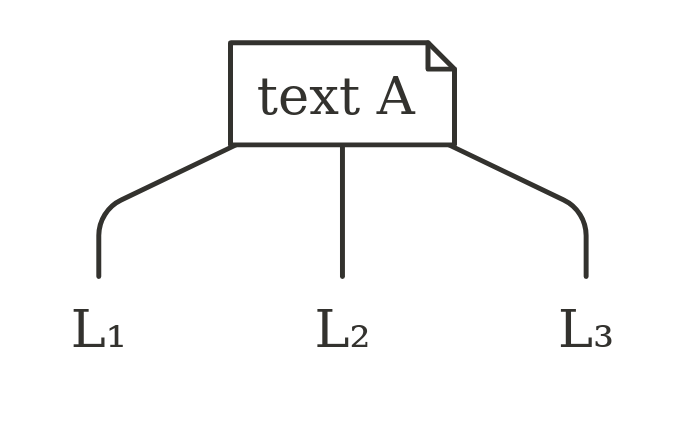
\includegraphics[width=.7\linewidth]{figure/scen1.png}
    \end{subfigure}%
    \begin{subfigure}{.5\textwidth}
        \centering
        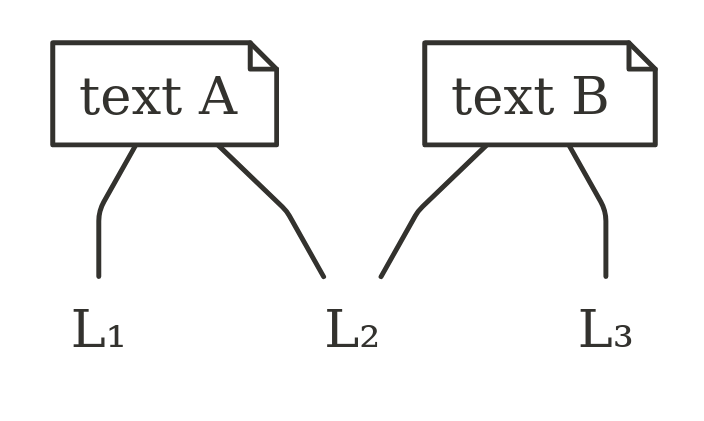
\includegraphics[width=.7\linewidth]{figure/scen2.png}
    \end{subfigure}
    \caption[The two CP scenarios compared]{The two CP scenarios compared. On the left, Scenario 1, when CP is applied on three translations of the same text. On the right, Scenario 2, dealing with two distinct bilingual texts.}
    \label{scens}
\end{figure}

Our algorithm is meant to be as general as possible, and as such it is not optimized for the first scenario, but rather covers both without making any assumptions in terms of sentence alignment\footnote{A way to make the algorithm more efficient for the first scenario could in fact be to rely on the fact that the $n$-lingual parallel text is sentence-aligned, keep track of the sentence from which a particular concept has been extracted and only try to find a equivalent in the corresponding $L_3$ sentence.}. 
It works as follows: for each alignment obtained by performing CE on text $A$, we consider the dependency tree in language $L_2$. We then look for such tree among all subtrees the $L_2$ version of text $B$ is composed of. If a sentence in the $L_2$ version of text $B$ does contain $a_i^2$, we align such sentence to its $L_3$ counterpart using the same procedure as described in Section \ref{extrain} for CE. Finally, if multiple possible correspondences are found, the $L_3$ dependency subtree which is closest in depth to $a_i^2$ is selected. This is meant to avoid, for instance, mistakenly aligning a full sentence tree to a dependency tree extracted when aligning heads, which would otherwise be likely, as their heads are obviously both labelled \texttt{root}. In the next two sections, we discuss some important details of the algorithm, and in Section \ref{heads2} in particular will get to other issues related to head alignment.

\begin{figure}[H]
    \centering
    \lstinputlisting{pseudocode/Propagate.hs}
    \caption[The CP algorithm]{The CP algorithm. The concept to propagate is looked for among the SL subtree of each alignment obtained by comparing the sentences of the new corpus. If it is found, the alignment it belongs to is returned. If there are multiple possible alignments, the alignment whose TL side is closest in depth to the concept itself is returned.}
    \label{prop}
\end{figure}

\subsection{Ignoring details of UD trees}
One point that becomes of extreme importance when dealing with Scenario 2, i.e. when the text used for CP is not a translation of the one used for CE, is the way we look for subtrees in the $L_2$ version of text $B$. Since we work with two different $L_2$ texts, in fact, we cannot expect text $B$'s subtrees to match $L_2$ concepts extracted from $T_1$ exactly: as we saw in Section \ref{ce}, nodes of UD trees contain information, particularly about the position of each word and its head, that should be disregarded in this context.\smallskip 

To make the CP algorithm more robust to minor parse errors, our decision was to consider two (sub)trees equivalent based on a comparison of just their shape and their \texttt{FORM}, \texttt{LEMMA}, \texttt{UPOS} and \texttt{DEPREL} fields. 
In this way, not only all optional fields (which might well differ or be blank for only one of the texts), but word position information is also ignored. 

\subsection{Propagating head alignments} \label{heads2}
The propagation of head alignments is by far the most challenging aspect of CP. 
This is due to the fact that the head of a dependency tree $t$, as defined for the purposes of CE (cf. Section \ref{heads}), is not, strictly speaking, a subtree of $t$ (even though in a broader sense it is, of course, a part of $t$). When head alignments are extracted, in fact, their members are either: \smallskip

\begin{itemize}
    \item trees composed exclusively of the root of a dependency subtree
    \item trees composed of the root of a dependency subtree and some of its immediate subtrees. As discussed in Section \ref{heads}, this happens in cases such as when the root in the SL is a compound (written as a one-word) and its TL counterpart is a multiword.
\end{itemize} \smallskip

Not only, then, is it necessary to look for each concept to propagate among all the dependency subtrees of each SL sentence of the corpus CP is performed on, but for each subtree it is also necessary to check whether the concept could be a head of such subtree. This is implemented by means of a function \texttt{isHeadOf} specular to \texttt{alignHeads}. \smallskip

If this is the case, i.e. if the concept the program is trying to propagate is the head of a certain SL subtree, then the resulting alignment should be with the head of the TL counterpart of such subtree.

\section{Evaluation} \label{eval3}
In the following three sections, we describe both the CP experiments performed and their results. Clearly, for all the experiments, we make use of the evaluation script used for CE, which has been extended to also compute CP-specific statistics, such as the percentage of (successfully) propagated concepts.

\subsection{Preliminary testing} 
One way to check the CP module for obvious flaws before trying to assess its performance in the two scenarios described above is to try to re-obtain the alignments obtained with the CE module via propagation. This means running both programs on the exact same input treebanks as used for CE. It represents a special case of Scenario 1 in which the program is expected to be able to propagate all alignments, with no exceptions. \smallskip 

The fact that many of the alignments obtained via propagation are the same as the ones extracted initially is generally a good indication that the program is working according to expectations. However, this has to be taken with a grain of salt: as discussed in the above, the program looks for one possible counterpart per concept only and is provided no indication about what sentence in particular it should look into, so that in presence of multiple valid alternative alignments the user should not expect it to identify the same correspondences as the extraction procedure, but rather just correct, potentially different correspondences. 

\subsubsection{Experimental results} \label{eval4r}
This kind of pre-evaluation has been run on the first 100 sentences of the PUD treebanks in English and Italian, one of the corpora used for evaluating CE. Most importantly, the experiment confirms that the CP module is in fact able to find all the alignments extracted by CE. 
The results also show that the vast majority of the propagated alignments is identical to its extracted counterpart, and that most often, even when it is not, that does not imply that the propagated alignment is incorrect. Out of a total of 224 (18.69\%) incorrect propagated alignments, only 28 (12.5\%) introduce an alignment error which was not already present in their extracted counterparts, and there are even instances where propagated alignments are, conincidentally, correct even though their extracted counterparts are not.

\subsection{Scenario 1}
For evaluating how well CP works in the first scenario, the corpus we use is the same as for testing, but in three instead of two languages: the concept extracted by means of comparing the English to the Italian version are propagated to Swedish, using both English and Italian UD trees as the starting point. \smallskip

Considering that we are working with three versions of the same text, the expectation is for the program to be able to propagate the vast majority of the concepts with a precision similar to that obtained during the extraction stage, even though free translation, unhandled translation divergences and annotation inconsistencies can make it possible for some of them not to be found in the Swedish translation or not to be aligned correctly. \smallskip

As for when it comes for CE, comparing the results of CP for two different language pairs, English-Swedish and Italian-Swedish, can be interesting to see how much easier it is to propagate concepts in two more syntactically similar languages.

\subsubsection{Experimental results}
As Table \ref{tcp1} shows, the experimental results of this type of evaluation match the above expectations. First, the number of alignments the program is able to propagate is, for both language pairs, smaller than that obtained in the testing phase but still relatively large, while the amount of propagation errors increases marginally. Furthermore, the English-Swedish pair gives slightly better results than the Italian-Swedish pair, both in terms of the number of alignments the program is able to propagate and in terms of the amount of alignment errors. \smallskip

It is interesting to notice, however, that the amount of errors is significantly (> 5\%) inferior when concepts are propagated to Swedish starting from English, as opposed to Italian, dependency trees. This is most likely due to the syntactical features shared by the former two languages. This means that not all Italian-English extraction errors are propagated and it seems to suggest that, if we were to only use the trilingual alignments obtained by English-Italian extraction followed by English-Swedish propagation, some of the initial incorrectly extracted alignments would be automatically discarded.

\begin{table}[H]
    \centering
    \begin{tabular}{|l|l|l|}
    \hline
    \textbf{}              & \textbf{en-sv} & \textbf{it-sv} \\ \hline
    \textbf{propagated}             & 1019 (85.05\%) & 979 (84.64\%) \\ \hline
    \textbf{tot. errors}            & 133 (13.05\%)  & 187 (19.1\%)  \\ \hline
    \textbf{CP-introduced}          & 75 (56.39\%)   & 84 (44.91\%)   \\ \hline
    \end{tabular}
    \caption[Performance of CP Scenario 1 on manually annotated data]{Results of propagating the Italian-English alignments obtained via CE on the first 100 sentences of the PUD corpus to Swedish, using either the English or Italian subtrees as a starting point.}
    \label{tcp1}
    \end{table}

\subsection{Scenario 2}

The PUD corpus is composed of extracts of texts on a variety of subjects. As a consequence, performing an evaluation of CP in Scenario 2 using, for extraction and propagation, two different subsets of the corpus, would not help assess whether the module is well suited for the most relevant subcase of such scenario, i.e. when working with two texts belonging to the same domain. \smallskip

On top of evaluating the program on PUD data dividing the set of sentences used so far into two equally sized subsets, then, the two course plans corpora described in Section \ref{plans} have been also used to put the program to the test. \smallskip

These two small bilingual corpora allow us to perform two additional experiments: \smallskip
\begin{enumerate}
    \item to extract English-Swedish alignments from the CSE corpus and propagate them to Italian using the DMI corpus
    \item vice versa, to extract English-Italian alignments from the DMI corpus and propagate them to Swedish using the CSE corpus
\end{enumerate} \smallskip

\subsubsection{Experimental results}

\paragraph{Propagation with texts in different domains}
When it comes to the first set of experiments, where we use PUD data, being the subsets of selected sentences extremely small and having the correctness of most alignments been already assessed in previous experiments, it is easy to work with all possible pairs of languages. The results, summarized in Table \ref{tcp2pud}, show that, in general, only a small fraction of the extracted alignments are actually propagated in this case. As mentioned above, this is to be expected since different sentences belong to different domain. A closer look to the set of alignments returned by propagation, the vast majority of which has single words as members, shows that most of them are common function words, which, alone, are not always relevant for a GF-based MT pipeline. 
Common determiners such as articles, for instance, can be better handled by RGL grammars alone. 
Prepositions, on the other hand, are only useful with some information about the context in which they occur in, since it is customary for them to be used differently across different, even closely related languages. 
However, some common content words, like $\langle$\textit{``always'', ``sempre'', ``alltid''}$\rangle$, $\langle$\textit{``new'', ``nuovi'', ``nya''}$\rangle$ and $\langle$\textit{``same'', ``stesso'', ``samma''}$\rangle$ are also aligned correctly.

\begin{table}[H]
    \centering
    \scriptsize
    \begin{tabular}{|l|l|l|l|l|l|l|}
    \hline
    \textbf{}                     & \textbf{en-it-sv} & \textbf{it-en-sv} & \textbf{en-sv-it} & \textbf{sv-en-it} & \textbf{it-sv-en} & \textbf{sv-it-en} \\ \hline
    \textbf{extracted}   & 638               & 638               & 687               & 687               & 608               & 608               \\ \hline
    \textbf{propagated}                    & 92 (14.42\%)      & 92 (14.42\%)      & 98 (14.26\%)      & 84 (12.22\%)      & 101 (16.61\%)     & 87 (14.37\%)      \\ \hline
    \textbf{tot. errors}                   & 46 (50\%)         & 21 (22.82\%)      & 42 (42.85\%)      & 24 (28.57\%)      & 21 (20.79\%)      & 28 (32.18\%)      \\ \hline
    \textbf{CP-introduced}                 & 33 (71.73\%)      & 11 (52.38\%)      & 21 (50\%)         & 12 (50\%)         & 12 (57.14\%)      & 21 (75\%)         \\ \hline
    \end{tabular}
    \caption[Performance of CP Scenario 2 on manually annotated non-homogeneous data]{Results of CP for various language pairs using PUD (non-homogeneous) data. For each column, the first two languages are the ones used for extraction and the second two the ones used for propagation.}
    \label{tcp2pud}
    \end{table}

The table also shows, like the results obtained from Scenario 1 suggest too, that the order in which languages are used is not completely irrelevant: while the percentage of propagated alignments does not vary widely, the amount of errors is significantly lower when the propagation step involves the two syntactically more similar languages, English and Swedish. The fact that CP works better with English-Italian than with Italian-Swedish, on the other hand, may simply be a result of the fact that the latter language pair was never used for testing the program during its development, which might have caused some of the criteria to be not completely language pair-independent. \smallskip

Finally, the percentage of errors introduced by CP is significantly higher than that recorded for Scenario 1. One factor that contributes to this is the fact that function words, which are by far more numerous in the propagated alignments than content words, are often used differently in different languages and contexts. When it comes to the languages we are considering, this applies in particular to prepositions: because it is hard to know what the correct translation equivalent is without looking at the specific sentence, when CP is performed on a text different from the one used for CE, many preposition-to-preposition alignments have to be marked as incorrect even though they might be correct in some specific cases.

\paragraph{Propagation with texts within the same domains}

Quantitatively, the results of the last pair of experiments, performed on two different automatically parsed bilingual corpora composed of course plans of Computer Science programmes, are to some extent similar to those obtained using different texts in different domains (cf. Tables \ref{tcp2courses} and \ref{tcp2pud}). Only a tiny fraction of the extracted alignments is propagated and errors are numerous, as in the previous setting. 

\begin{table}[H]
    \centering
    \begin{tabular}{|l|l|l|}
    \hline
                           & \textbf{sv-en-it} & \textbf{it-en-sv} \\ \hline
    \textbf{extracted}     & 1950              & 1823              \\ \hline
    \textbf{propagated}             & 205 (10.51\%)     & 200 (10.97\%)     \\ \hline
    \textbf{tot. errors}            & 66 (32.19\%)      & 61 (30.5\%)       \\ \hline
    \textbf{CP-introduced} & 33 (50\%)        & 33 (54.09\%)      \\ \hline
    \end{tabular}
    \caption[Performance of CP Scenario 2 on automatically parsed homogeneous data]{Results of CP for using two different bilingual corpora belonging to the same domain of course plans. For each column, the first two languages are the ones used for extraction and the second two the ones used for propagation.}
    \label{tcp2courses}
    \end{table}

    More than the quantitative results, however, it is interesting to take a look at some of the propagated concepts. Because the text are similar both stylistically and, most importantly, in terms of content, the program is in this case also able to find trilingual correspondences between content words, sometimed specific of the domain. 
    
    Examples of such alignments are $\langle$\textit{``skills'', ``capacità'', ``färdigheter''}$\rangle$, $\langle$\textit{``functional'', ``funzionale'', ``funktionell''}$\rangle$, $\langle$\textit{``exam'', ``prova'', ``tentamen''}$\rangle$, $\langle$\textit{``course'', ``corso'', ``kurs''}$\rangle$, $\langle$\textit{``lectures'', ``lezioni'', ``föreläsningar''}$\rangle$, $\langle$\textit{``prerequisites'', ``prerequisiti'', ``behörigheter''}$\rangle$ and $\langle$\textit{``knowledge'', ``conoscenza'', ``kunskap''}$\rangle$. \smallskip

    Sometimes, however, the meaning of a word is highly context-dependent and as a consequence, even if both the pairs of extracted and propagated alignments are correct, the corresponding trilingual alignment we could infer isn't (e.g. $\langle$\textit{``learning'', ``conoscere''}$\rangle$ and $\langle$\textit{``learning'', ``inlärning''}$\rangle$). \smallskip

    Finally, in some rare cases, even correspondences regarding longer expressions, such as $\langle$\textit{``the aim of the course'', ``l'obiettivo del corso'', ``syftet med kursen''}$\rangle$, can be found. In this case, the English-Italian correspondence is not especially useful, since the phrase could be translated almost word by word between the two languages, but the translation to Swedish is not literal, thus making the alignment useful for the purposes of MT.

% CONCEPT ALIGNMENT IN MACHINE TRANSLATION
\chapter{Concept Alignment in Machine Translation} \label{ch5}
We conclude this work by documenting a first attempt to put our CA component to use in a MT system. 
The chapter starts with a discussion of how GF translation can benefit from using concepts extracted with our method as translation units.
After that, we give a step-by-step description of how this is achieved, also indicating the changes made to the CA module to adjust it for this specific use case. 
Finally, Section \ref{eval5} focuses on the actual evaluation of the resulting system and presents its results.

\section{Method and implementation}
As discussed in Section \ref{gf}, GF translation consists in parsing SL strings to obtain the corresponding ASTs to then linearize them according to the concrete syntax of the TL.
As well as describing the morphological and syntactical features of the languages involved, a multilingual grammar suited for this task defines a \textit{translation lexicon}, i.e. a set of word senses and the corresponding expressions in the various languages. \smallskip

Automating CA can be seen, then, as a first step for automatically generating such lexicon. 
An important point is that our approach, as opposed to word alignment techniques, identifies concepts at different levels of abstraction.
This allows us to construct lexical entries not only for the grammatical categories that typically correspond to single words (such as nouns, adjectives and adverbs), but also for phrases (with the term ``phrase'' now intended grammatically, as opposed to its meaning in SMT).
Doing so enables GF translation, designed to preserve grammatically, to also render idiomatic expressions found in the data used for generating the lexicon correctly. \smallskip

Obtaining a multilingual GF grammar from a set of aligned UD trees, however, is not immediate. In the following three sections, we illustrate the different steps of this process. We then introduce the simple GF-based MT module used for the experiments discussed in Section \ref{eval5} and describe the adjustments made to the CA component in order to optimize it for the task at hand. 

\subsection{UD-to-GF conversion}
The output of both CE and CP is, unless when linearized for evaluation purposes, a set of aligned UD trees in CoNNL-U format. In order to be used for GF-based translation, such trees need to be first converted into GF ASTs, which are then used to generate a set of grammar rules constiuting the above mentioned multilingual GF lexicon. \smallskip

Conversion is based on annotations defining the relation between UD trees and GF ASTs, which we refer to as \textit{dependency configurations}. 
While going into all the notational details is beyond the scope of this project\footnote{a comprehensive description of \texttt{gf-ud}'s annotation scheme is available at \url{github.com/GrammaticalFramework/gf-ud/blob/master/doc/annotations.md}.}, an example of one such configuration is 

\begin{verbatim}
    #fun PredVP	nsubj head
\end{verbatim}

which specifies that a \texttt{PredVP} (predicative Verb Phrase), defined in the RGL as a function of type

\begin{verbatim}
    PredVP : NP -> VP -> Cl
\end{verbatim}

i.e. a function taking two arguments, an \texttt{NP} (Noun Phrase) and a \texttt{VP} (Verb Phrase) and returning a \texttt{Cl} (clause), corresponds to a UD tree whose head, the VP, has a \texttt{nsubj} attached to it. Appendix \ref{c} lists the dependency configurations used for UD-to-GF conversion in the context of this project.
\smallskip

As discussed in Section \ref{udrelgf}, the UD-to-GF conversion, while being more complex than its reverse, can be performed by \texttt{gf-ud}, a program offering several functionalities useful to work with GF and UD simultaneously.
Such program, however, cannot be fed the alignments obtained via CE and CP directly. This is due to the fact that the members of most of the relevant alignments are subtrees (or heads of subtrees) and not complete UD trees. 
While this makes no difference in terms of the Haskell data type we represent them with (cf. Figure \ref{types}), trying to print them to files in the corresponding CoNNL-U notation with no postprocessing leads to malformed UD sentences. \smallskip

The problem, which is due to the lack of a root labelled as such and illegal \texttt{ID} and \texttt{HEAD} values, was solved by implementing a simple normalization procedure, now part of the CA library. 
Called every time a UD subtree has to be converted to CoNNL-U, it first replaces the UD label (\texttt{udDEPREL}) of its root node with \texttt{root} and assigns the special value 0 to its \texttt{udHEAD} field. After that, it proceeds to ``rescale'' the \texttt{udID} and \texttt{udHEAD} fields of all other nodes so that they end up into the range $[1,n]$, where $n$ is the number of nodes of the extracted subtrees\footnote{see Section \ref{conll} and Figure \ref{types} for definitions of all the fields of UD trees and their CoNNL-U representations.}. \smallskip

\begin{figure}[H]
\small
\begin{Verbatim}[commandchars=\\\{\}]
\textcolor{gray}{   
    1  sadly  sadly  ADV  _  _  5  advmod  _  _}
    2  this  this  DET  _  _  4  det  _  _
    3  malformed  malformed  ADJ  _  _  4  amod  _  _
    4  subtree  subtree  NOUN  _  5  nsubj  _  _
    \textcolor{gray}{5  needs  need  VERB  _  _  0  root  _  _}
    \textcolor{gray}{6  postprocessing  postprocess  VERB  _  _  5  xcomp}

\end{Verbatim}
\centering
\large
$\Downarrow$
\small
\begin{verbatim}


    1	this	this	DET	_	_	3	det	_	_
    2	malformed	malformed	ADJ	_	_	3	amod	_	_
    3	subtree	subtree	NOUN	_	_	0	root	_	_
\end{verbatim}
\caption[A UD subtree and its normalization]{A vanilla noun phrase subtree (highlighted in black) in the context it was extracted from (gray) and the same subtree after normalization.}
\label{normalization}
\end{figure}

Another practical problem that arises when trying to transform a CoNNL-U tree into a GF AST is that \texttt{gf-ud} easily becomes remarkably resource-intensive when dealing with ambiguous, large trees. 
This is due to the fact that conversion in this direction is a nondeterministic search problem \cite{udgf}. 
For this reason, it can be useful to limit the size\footnote{in this context, the size of an alignment is defined as the number of nodes of its largest member.} of the alignments that are actually kept after the extraction (or propagation) procedure. Since our CA component works at all levels of abstraction, thus also aligning full clauses, this turned out to be essential and became one of the command-line parameters of the final executables, as mentioned in Appendix \ref{b}. \smallskip

\subsection{Grammar generation} \label{grgn}
The result of this UD-to-GF conversion is still a series of tree alignments, but their resulting format makes a substantial difference, since GF ASTs can be used to obtain the rules of a generative grammar. \texttt{gf-ud} also provides a way to do this, given an \textit{extraction grammar} and a \textit{morphological dictionary} of the languages of the alignments. \smallskip

What we refer to as an \textit{extraction grammar} is of course a GF grammar, whose objective is to define the set of basic categories and syntactic rules the entries of the automatically generated GF lexicon is going to be based on. \smallskip

A \textit{morphological dictionary}, on the other hand, contains correspondences between a large number of lemmas and various word forms. In this case, the morphological dictionaries themselves are implemented in GF. \smallskip

The program responsible for generating the GF lexicon given these components has been written in parallel with - but not as part of - this thesis project and is still under development. As a consequence, some programming work was required to automate the few parts of the process that still had to be performed manually and some (minimal) postprocessing is sometimes required before the automatically generated grammars can be compiled. This happens for instance when Italian words are incorrectly POS-tagged as verbs and, not having a word ending typical of such category, produce pattern matching errors when the corresponding strings are passed to the constructor generating all the verb forms. \smallskip

\subsubsection{Extending the extracted grammar} \label{extend}
The extraction grammar is designed for the grammar generation module to produce grammar rules corresponding to small concepts: basic categories, noun phrases, verb phrases etc. 
As a consequence, if used directly, grammars resulting from the above described generation step can only deal with very simple predicative sentences, with verbs in the present tense of the indicative mood, and their constituents, such as\smallskip

\begin{example}
    ``this sentence is simple''
\end{example}

Of course, some limited variation is still possible. For instance, the determiner can change or disappear, number can vary, the complement of the copula can become a noun and an adjectival modifiers and prepositional phrases can be added to each noun phrase. For instance:

\begin{example} \ 
    \begin{itemize}
        \item ``the sentence is simple''
        \item ``a sentence is simple''
        \item ``sentences are simple''
        \item ``these sentences are simple''
        \item ``this sentence is an example''
        \item ``this short sentence is simple''
        \item ``this sentence of the text is simple''
    \end{itemize}
\end{example}

For languages that are covered by the RGL, however, it is also extremely easy to extend such grammars with preexisting syntax rules so to make it possible to generate more complex clauses and sentences and add useful function words. The grammars used for the experiments that will be described in Section \ref{eval5}, for example, have been extended also to cover negative and interrogative forms, the past and future tense of verbs in the indicative mood and comparative adjectives. This allows for plenty of variations, such as:

\begin{example} \
    \begin{itemize}
        \item ``this sentence isn't simple''
        \item ``is this sentence simple?''
        \item ``this sentence was simple''
        \item ``this sentence will be simple''
        \item ``this sentence is simpler than that sentence''
    \end{itemize}
\end{example}

Of course, variations can be combined, so that the grammar can produce sentences like the following:

\begin{example}
    ``Won't these short sentences be simpler than that long sentence?''
\end{example}

This is accomplished by making the automatically generated grammars extend not only the extraction grammar itself, but also a module that simply imports the necessary standard RGL categories and functions.

\subsection{Translation} \label{mt}
Maybe counterintuitively, the MT module itself is by far the simplest component of the entire system. Built using PGF, the API meant to be used for embedding GF grammars in Haskell programs, it simply makes use of GF parsing and linearization.
The only difference between translating inside the GF shell and using this ad-hoc program, apart from the increased ease of use of the latter, are that: \smallskip

\begin{itemize}
    \item while GF can parse the SL string in a variety of ways and, as a consequence, return multiple TL linearizations, our program only outputs the first candidate translation, preliminarily discarding trees containing terminal nodes that have no linearization in the TL\footnote{a linearization can be missing, for instance, if a concrete syntax is postprocessed by simply getting rid of an ``illegal'' verb causing compilation problems (cf. Section \ref{grgn})} 
    \item to facilitate the experiments, our standalone program can translate several newline-separated sentences at once.
\end{itemize}

\subsection{Adjustments to the CA component} \label{tuning}

While the domain of application of CA we focus on in this work is automatic translation, the system described so far is not in any way optimized for it and can also be made use of in other contexts. 
For instance, it is easy to imagine using it to improve the user interface of online translation memories or to facilitate reading parallel texts in the context of language learning. \smallskip

In our particular setting, however, some practical problems arise and some adjustments can be done in order to make the CA software more well suited to the generation of a translation lexicon. \smallskip

In the following section, we discuss two ways to mitigate the impact of the annotation errors that inevitably derive from applying automatic dependency parsing on raw, possibly noisy data. Both techniques aim to increase the number of extracted alignments without significantly affecting precision.
Section \ref{select}, going in a sense in the opposite direction, describes the strategies we apply to filter out irrelevant alignments.

\subsubsection{Dealing with parse errors}
As discussed in Sections \ref{eval2} and \ref{eval3}, both our CE and CP modules give promising results on manually annotated data. However, when run on UDPipe-generated dependency trees, performance, and recall in particular, is significantly affected by errors happening at the parsing stage. Because parsing itself is a process consisting of several stages, errors differ based on when they happen. In particular, UDPipe goes through the following steps, each potentially causing one ore more particular kinds of errors: \smallskip

\begin{enumerate} 
    \item \textit{\textbf{tokenization}}, which can, although it is unlikely for the languages considered in this work, lead to errors in identifying word boundaries
    \item \textit{\textbf{morphological analysis}}, which can cause lemmatization and, consequently, POS-tagging errors
    \item actual \textit{\textbf{dependency parsing}}, the potential cause of attachment and labelling errors
\end{enumerate} \smallskip

In this context, we focus on the syntax-level errors: attachment and labelling. Of course, lemmatization and POS-tagging errors can be the first cause of one such error. In particular, the fact that a word is lemmatized incorrectly can make it so that it is also attributed the wrong POS tag and, as a consequence, assigned the wrong dependency label and/or attached to the wrong node. \smallskip

\begin{example}
    Consider the Italian sentence ``quel fa è diesis'' (``that F is sharp'').
    Notoriously, in Italian, the word ``fa'' can stand for the musical note F. Since ``fa'' is also the third person singular of the present indicative of the verb ``fare'' (``to do'', ``to make''), it is likely to be lemmatized so (instead of as ``fa''). If so, it will also probably POS-tagged as a \texttt{VERB} and assigned a dependency label typical of verbs (in this case, with no other lexical verbs in the sentence, most likely \texttt{root}, thus producing an attachment error as well), while the correct annotation is

    \begin{figure}[H]
        \begin{subfigure}{.5\textwidth}
            \centering
            \footnotesize
            \begin{verbatim}
    1	quel	quello	DET	_	_	2	det	_	_
    2	fa	fa	NOUN	_	_	4	nsubj	_	_
    3	è	essere	AUX	_	_	4	cop	_	_
    4	diesis	diesis	ADJ	_	_	0	root	_	_
            \end{verbatim}
        \end{subfigure}
        \begin{subfigure}{.5\textwidth}
            \centering
            \footnotesize
            \begin{picture}(223.0,90.0)
                \put(0.0,0.0){quel}
                \put(46.0,0.0){fa}
                \put(92.0,0.0){è}
                \put(129.0,0.0){diesis}
                \put(0.0,15.0){{\tiny DET}}
                \put(46.0,15.0){{\tiny NOUN}}
                \put(92.0,15.0){{\tiny AUX}}
                \put(129.0,15.0){{\tiny ADJ}}
                \put(33.0,30.0){\oval(39.47826086956522,33.333333333333336)[t]}
                \put(13.26086956521739,35.0){\vector(0,-1){5.0}}
                \put(18.0,49.66666666666667){{\tiny det}}
                \put(97.5,30.0){\oval(79.3855421686747,66.66666666666667)[t]}
                \put(57.80722891566265,35.0){\vector(0,-1){5.0}}
                \put(82.5,66.33333333333334){{\tiny nsubj}}
                \put(120.5,30.0){\oval(28.89189189189189,33.333333333333336)[t]}
                \put(106.05405405405405,35.0){\vector(0,-1){5.0}}
                \put(105.5,49.66666666666667){{\tiny cop}}
                \put(144.0,90.0){\vector(0,-1){60.0}}
                \put(149.0,80.0){{\tiny root}}
              \end{picture}
        \end{subfigure}
    \end{figure}
\end{example}
\smallskip

Nontheless, because we do not want to intervene on the parser directly (nor to modify its results), we ignore the causes and focus on the syntax-level errors directly. \smallskip

\paragraph{Working at the clause level} \label{clauses}
At the highest level of abstraction, the parser often fails to correctly identify the clauses a sentence is composed of. This happens in a variety of ways: at times, clauses are simply not identified as such or, on the contrary, non-clauses are labelled as clauses. 
Most often, however, clauses are simply not attached to the right node and/or given a label that, while still identifying them as clauses, does not give correct information about their type. \smallskip

To address this problem, the CE module has been modified so that it can try to align individual clauses instead of sentences. The idea is to obtain, from each pair of sentence trees to align, a pair of lists of subtrees whose heads are labelled \texttt{root}, \texttt{csubj}, \texttt{ccomp}, \texttt{xcomp}, \texttt{advcl} or  \texttt{acl}\footnote{all these clausal labels are defined in Appendix \ref{a_lab}}.

\begin{figure}[h]
\footnotesize
\setlength{\unitlength}{0.222mm}
\begin{picture}(817.0,150.0)
  \put(0.0,0.0){this}
  \put(46.0,0.0){sentence}
  \put(128.0,0.0){\textbf{shows}}
  \put(183.0,0.0){how}
  \put(220.0,0.0){to}
  \put(266.0,0.0){\textbf{work}}
  \put(312.0,0.0){at}
  \put(349.0,0.0){the}
  \put(386.0,0.0){clause}
  \put(450.0,0.0){level}
  \put(505.0,0.0){to}
  \put(551.0,0.0){\textbf{increase}}
  \put(633.0,0.0){recall}
  \put(0.0,15.0){{\tiny DET}}
  \put(46.0,15.0){{\tiny NOUN}}
  \put(128.0,15.0){{\tiny \textbf{VERB}}}
  \put(183.0,15.0){{\tiny ADV}}
  \put(220.0,15.0){{\tiny PART}}
  \put(266.0,15.0){{\tiny \textbf{VERB}}}
  \put(312.0,15.0){{\tiny ADP}}
  \put(349.0,15.0){{\tiny DET}}
  \put(386.0,15.0){{\tiny NOUN}}
  \put(450.0,15.0){{\tiny NOUN}}
  \put(505.0,15.0){{\tiny PART}}
  \put(551.0,15.0){{\tiny \textbf{VERB}}}
  \put(633.0,15.0){{\tiny NOUN}}
  \put(33.0,30.0){\oval(39.47826086956522,33.333333333333336)[t]}
  \put(13.26086956521739,35.0){\vector(0,-1){5.0}}
  \put(18.0,49.66666666666667){{\tiny det}}
  \put(97.0,30.0){\oval(78.34146341463415,33.333333333333336)[t]}
  \put(57.829268292682926,35.0){\vector(0,-1){5.0}}
  \put(82.0,49.66666666666667){{\tiny nsubj}}
  \put(234.5,30.0){\oval(79.3855421686747,66.66666666666667)[t]}
  \put(194.80722891566265,35.0){\vector(0,-1){5.0}}
  \put(219.5,66.33333333333334){{\tiny advmod}}
  \put(253.0,30.0){\oval(39.47826086956522,33.333333333333336)[t]}
  \put(233.26086956521738,35.0){\vector(0,-1){5.0}}
  \put(238.0,49.66666666666667){{\tiny mark}}
  \put(217.0,30.0){\oval(135.82608695652175,100.0)[t]}
  \put(284.9130434782609,35.0){\vector(0,-1){5.0}}
  \put(202.0,83.0){{\tiny \textbf{xcomp}}}
  \put(391.0,30.0){\oval(135.82608695652175,100.0)[t]}
  \put(323.0869565217391,35.0){\vector(0,-1){5.0}}
  \put(376.0,83.0){{\tiny case}}
  \put(409.5,30.0){\oval(98.02970297029702,66.66666666666667)[t]}
  \put(360.4851485148515,35.0){\vector(0,-1){5.0}}
  \put(394.5,66.33333333333334){{\tiny det}}
  \put(428.0,30.0){\oval(59.3125,33.333333333333336)[t]}
  \put(398.34375,35.0){\vector(0,-1){5.0}}
  \put(413.0,49.66666666666667){{\tiny nmod}}
  \put(378.0,30.0){\oval(182.3695652173913,133.33333333333334)[t]}
  \put(469.1847826086956,35.0){\vector(0,-1){5.0}}
  \put(363.0,99.66666666666667){{\tiny obl}}
  \put(538.0,30.0){\oval(39.47826086956522,33.333333333333336)[t]}
  \put(518.2608695652174,35.0){\vector(0,-1){5.0}}
  \put(523.0,49.66666666666667){{\tiny mark}}
  \put(428.5,30.0){\oval(283.94736842105266,166.66666666666666)[t]}
  \put(570.4736842105264,35.0){\vector(0,-1){5.0}}
  \put(413.5,116.33333333333333){{\tiny \textbf{advcl}}}
  \put(612.0,30.0){\oval(78.34146341463415,33.333333333333336)[t]}
  \put(651.170731707317,35.0){\vector(0,-1){5.0}}
  \put(597.0,49.66666666666667){{\tiny obj}}
  \put(143.0,150.0){\vector(0,-1){120.0}}
  \put(148.0,140.0){{\tiny \textbf{root}}}
\end{picture}
\begin{itemize}
    \item ``\textit{this sentence \textbf{shows} how to work at the clause level to increase recall}''
    \item ``\textit{how to \textbf{work} at the clause level to increase recall}''
    \item ``\textit{to \textbf{increase} recall}''
\end{itemize}
\caption[A sentence and its decomposition into clauses]{A sentence and its decomposition into clauses. Note how the sentence is not actually segmented, but rather used to obtain a set of subsentences, each having their main verb, marked in bold, as root.}
\end{figure}

These lists of ``clauses''\footnote{``clauses'' is in quotes since what we are referring to as a clause includes its subclauses too. This means that the sentence is not segmented into clauses in the literal sense of the term, but rather that one tree per verb is extracted from them.} are then sorted by dependency label and distance from the root, so that in the absence of annotation errors, when there is in fact an evident correspondence, they appear in the same position. Finally, the program tries to align every possible pair of clauses and the pruning procedure described in \ref{pruning} is applied to only keep the ones that are more likely to be correct.

\paragraph{Dealing with unaligned subtrees} \label{exclusion}
Clearly, however, parse errors do not happen exclusively at the clause level: smaller units, e.g. verb arguments, can also be misclassified or attached to the wrong node. To partially work around the problem, the CE module supports what one could refer to as ``alignment by exclusion'': after the extraction procedure described in Section \ref{improvements} - or its modified version outlined in the above paragraph - is carried out, the program can try to find correspondences between the remaining unaligned subtrees. 
The idea is the same as above: subtrees are sorted, aligned and lastly alignments are pruned.
This is done ignoring, if necessary, the context in which the subtrees occur and potentially making only use of a subset of the alignments criteria, for instance the strictest and safest ones. \smallskip

This is useful in cases such as that illustrated in Figure \ref{rest}, as well as in the event of actual attachment ambiguity or when the two versions of the text present syntactical differences that cannot be handled with the simple divergence patterns introduced in Section \ref{divs}.

\begin{figure}[h]
    \centering
    \footnotesize
    \begin{subfigure}{.5\textwidth}
      \centering
      \setlength{\unitlength}{0.2mm}
      \begin{picture}(315.0,110.0)
        \put(0.0,0.0){parse}
        \put(55.0,0.0){this}
        \put(101.0,0.0){sentence}
        \put(183.0,0.0){with}
        \put(229.0,0.0){care}
        \put(0.0,15.0){{\tiny VERB}}
        \put(55.0,15.0){{\tiny DET}}
        \put(101.0,15.0){{\tiny NOUN}}
        \put(183.0,15.0){{\tiny ADP}}
        \put(229.0,15.0){{\tiny NOUN}}
        \put(88.0,30.0){\oval(39.47826086956522,33.333333333333336)[t]}
        \put(68.26086956521739,35.0){\vector(0,-1){5.0}}
        \put(73.0,49.66666666666667){{\tiny det}}
        \put(70.5,30.0){\oval(98.02970297029702,66.66666666666667)[t]}
        \put(119.51485148514851,35.0){\vector(0,-1){5.0}}
        \put(55.5,66.33333333333334){{\tiny obj}}
        \put(216.0,30.0){\oval(39.47826086956522,33.333333333333336)[t]}
        \put(196.26086956521738,35.0){\vector(0,-1){5.0}}
        \put(201.0,49.66666666666667){{\tiny case}}
        \put(134.5,30.0){\oval(227.68995633187774,100.0)[t]}
        \put(248.34497816593887,35.0){\vector(0,-1){5.0}}
        \put(119.5,83.0){{\tiny obl}}
        \put(15.0,110.0){\vector(0,-1){80.0}}
        \put(20.0,100.0){{\tiny root}}
      \end{picture}
    \end{subfigure}%
    \begin{subfigure}{.5\textwidth}
        \centering
        \setlength{\unitlength}{0.25mm}
\begin{picture}(324.0,90.0)
  \put(0.0,0.0){analizza}
  \put(82.0,0.0){questa}
  \put(146.0,0.0){frase}
  \put(201.0,0.0){con}
  \put(238.0,0.0){cura}
  \put(0.0,15.0){{\tiny VERB}}
  \put(82.0,15.0){{\tiny DET}}
  \put(146.0,15.0){{\tiny NOUN}}
  \put(201.0,15.0){{\tiny ADP}}
  \put(238.0,15.0){{\tiny NOUN}}
  \put(124.0,30.0){\oval(59.3125,33.333333333333336)[t]}
  \put(94.34375,35.0){\vector(0,-1){5.0}}
  \put(109.0,49.66666666666667){{\tiny det}}
  \put(93.0,30.0){\oval(143.94520547945206,66.66666666666667)[t]}
  \put(164.97260273972603,35.0){\vector(0,-1){5.0}}
  \put(78.0,66.33333333333334){{\tiny obj}}
  \put(229.5,30.0){\oval(28.89189189189189,33.333333333333336)[t]}
  \put(215.05405405405406,35.0){\vector(0,-1){5.0}}
  \put(214.5,49.66666666666667){{\tiny case}}
  \put(212.0,30.0){\oval(88.73913043478261,66.66666666666667)[t]}
  \put(256.3695652173913,35.0){\vector(0,-1){5.0}}
  \put(197.0,66.33333333333334){{\tiny nmod}}
  \put(15.0,90.0){\vector(0,-1){60.0}}
  \put(20.0,80.0){{\tiny root}}
\end{picture}
    \end{subfigure}
    \caption[A case where alignment ``by exclusion'' is beneficial]{A case where alignment ``by exclusion'' is beneficial. In this case, while the two sentences should appear to be structured identically to a human reader, the Italian parse tree contains a (reasonable) attachment error. As a consequence, vanilla CE would not be able to align the prepositional phase ``\textit{with care}'', attached to the main verb ``\textit{parse}'', to its Italian exact counterpart ``\textit{con cura}'', incorrectly linked to the noun ``\textit{frase}'' as an \texttt{nmod}. A second CE pass trying to put unaligned subtrees in relation with each other, however, is able to detect the POS-equivalence between the two phrases, thus producing three new correct alignments: $\langle$\textit{with care, con cura}$\rangle$, $\langle$\textit{care, cura}$\rangle$ and $\langle$\textit{with, con}$\rangle$.}
    \label{rest}
\end{figure}

The results of this kind of optimization, however, as well as those of working at the clause level, vary widely depending on the quality of the parse trees and can be detrimental, in terms of precision, if applied to high-quality datasets.

\subsubsection{Selecting relevant alignments} \label{select}
The pruning procedure described in Section \ref{pruning} is aimed at filtering out alignments that, because of their number of occurrences and of the set of criteria thanks to which they have been extracted, are less likely to be correct. However, not all the alignments extracted in this way are relevant for the purposes of MT. \smallskip

On the one hand, most alignments that do not contain any content word are not useful for the generation of a domain-specific grammar, as many common function words are already covered by the GF RGL\footnote{small alignments containing both function and content words, such as prepositional phrases, are on the other hand extremely useful, as they show which specific function word should be used in a particular context.}. \smallskip 

On the other hand, the concepts represented in the GF grammar should intuitively, in most cases, be ``as small as possible''. If we reconsider the example in Figure \ref{cake} (sentences \textit{``finding useful correspondences is not exactly a piece of cake''} and \textit{``trovare corrispondenze utili non è proprio scontato''}), for instance, while the multi-word correspondence $\langle$\textit{a piece of cake, scontato}$\rangle$ is indeed useful there is usually no point in keeping correspondences such as $\langle$\textit{useful correspondences, corrispondenze utili}$\rangle$, even if they are correct, when it it also possible to extract the alignments $\langle$\textit{useful, utili}$\rangle$ and $\langle$\textit{correspondences, corrispondenze}$\rangle$: one-word and, in general, shorter alignments are more easily reusable in different contexts, especially since there are language-specific RGL rules capable of handling word order properly. 
As a consequence, for the purposes of grammar generation, the CA modules should in this case only return the following set of alignments: \smallskip

\begin{enumerate}
    \item $\langle$\textit{finding, trovare}$\rangle$
    \item $\langle$\textit{useful, utili}$\rangle$
    \item $\langle$\textit{correspondences, corrispondenze}$\rangle$
    \item $\langle$\textit{is, è}$\rangle$
    \item $\langle$\textit{not, non}$\rangle$
    \item $\langle$\textit{exactly, proprio}$\rangle$
    \item $\langle$\textit{a piece of cake, scontato}$\rangle$.
\end{enumerate} \smallskip

If we consider that the RGL can already handle most function words correctly, we can even discard all alignments that do not contain any content word (in this case, alignments 4 and 5, which leaves us with only 5 alignment useful to GF). \smallskip

In some situations, however, larger alignments (such as $\langle$\textit{useful correspondences, corrispondenze utili}$\rangle$) are considered to be relevant since they help understand which words can be safely used in conjunction with each other. For instance, while the Italian adjective ``\textit{brutto}'' (most often translated as ``\textit{ugly}'') is often used in conjunction with the word ``\textit{notizia}'' (``\textit{news}'') in expressions such as ``\textit{brutte notizie}'', in English the adjective ``\textit{bad}'' (as in ``\textit{bad news}'') is definitely more appropriate. Discarding a potential $\langle\textit{bad news}, \textit{brutte notizie}\rangle$ alignment is then not always the right choice, since in a context in which there are many alternative translation equivalents for the word ``\textit{brutto}'' it provides useful information about what adjective to use to refer to the noun ``\textit{news}''. \smallskip

Because of this, and since CE could have applications other than MT, selection in this sense is performed - optionally - after the extraction phase itself and implemented as an independent function. It works as follows: first, alignments that do not present any content word are filtered out. Then, among the remaining ones, \textit{superficially} perfect alignments \textit{containing} other extracted alignments are also discarded.\smallskip

To clarify such algorithm, it is worth defining perfect alignment - which was already mentioned in Section \ref{baseline} - more rigorously. \smallskip

\begin{definition}
    An alignment $A = \langle e_1,...,e_n \rangle$ is \textit{perfect} if its member dependency trees $e_1,...,e_n$ are identical both in their topology and in the dependency labels assigned to their nodes. 
\end{definition} \smallskip

The ``shallow'' version of perfect alignment the algorithm described above refers to, which we call \textit{superficially perfect alignment}, occurs when the definition applies at least to the roots of the two member trees and the roots of their immediate subtrees.\smallskip  

\begin{example}
    Consider the following pairs of English-Italian sentences:
    \begin{enumerate}
        \item $\langle$this algorithm selects \underline{the} relevant alignments, questo algoritmo seleziona gli allineamenti rilevanti$\rangle$
        \item $\langle$this algorithm selects relevant alignments, questo algoritmo seleziona gli allineamenti rilevanti$\rangle$
    \end{enumerate}

    While the two English sentences are translated to Italian in the same way, alignment is perfect only in the first case, where the determiner ``\textit{the}'' is present. The two trees are in fact identical if not for the words themselves and their order.

\begin{figure}[H]
    \centering
    \scriptsize
    \begin{subfigure}{.5\textwidth}
      \centering
      \setlength{\unitlength}{0.145mm}
\begin{picture}(479.0,110.0)
  \put(0.0,0.0){this}
  \put(46.0,0.0){algorithm}
  \put(137.0,0.0){selects}
  \put(210.0,0.0){the}
  \put(247.0,0.0){relevant}
  \put(329.0,0.0){alignments}
  \put(0.0,15.0){{\tiny DET}}
  \put(46.0,15.0){{\tiny NOUN}}
  \put(137.0,15.0){{\tiny VERB}}
  \put(210.0,15.0){{\tiny DET}}
  \put(247.0,15.0){{\tiny ADJ}}
  \put(329.0,15.0){{\tiny NOUN}}
  \put(33.0,30.0){\oval(39.47826086956522,33.333333333333336)[t]}
  \put(13.26086956521739,35.0){\vector(0,-1){5.0}}
  \put(18.0,49.66666666666667){{\tiny det}}
  \put(101.5,30.0){\oval(87.7032967032967,33.333333333333336)[t]}
  \put(57.64835164835165,35.0){\vector(0,-1){5.0}}
  \put(86.5,49.66666666666667){{\tiny nsubj}}
  \put(279.5,30.0){\oval(116.47899159663865,66.66666666666667)[t]}
  \put(221.26050420168067,35.0){\vector(0,-1){5.0}}
  \put(264.5,66.33333333333334){{\tiny det}}
  \put(298.0,30.0){\oval(78.34146341463415,33.333333333333336)[t]}
  \put(258.8292682926829,35.0){\vector(0,-1){5.0}}
  \put(283.0,49.66666666666667){{\tiny amod}}
  \put(253.0,30.0){\oval(190.4375,100.0)[t]}
  \put(348.21875,35.0){\vector(0,-1){5.0}}
  \put(238.0,83.0){{\tiny obj}}
  \put(152.0,110.0){\vector(0,-1){80.0}}
  \put(157.0,100.0){{\tiny root}}
\end{picture}
    \end{subfigure}%
    \begin{subfigure}{.5\textwidth}
        \centering
        \setlength{\unitlength}{0.16mm}
\begin{picture}(542.0,90.0)
  \put(0.0,0.0){questo}
  \put(64.0,0.0){algoritmo}
  \put(155.0,0.0){seleziona}
  \put(246.0,0.0){gli}
  \put(283.0,0.0){allineamenti}
  \put(401.0,0.0){rilevanti}
  \put(0.0,15.0){{\tiny DET}}
  \put(64.0,15.0){{\tiny NOUN}}
  \put(155.0,15.0){{\tiny VERB}}
  \put(246.0,15.0){{\tiny DET}}
  \put(283.0,15.0){{\tiny NOUN}}
  \put(401.0,15.0){{\tiny ADJ}}
  \put(42.0,30.0){\oval(59.3125,33.333333333333336)[t]}
  \put(12.34375,35.0){\vector(0,-1){5.0}}
  \put(27.0,49.66666666666667){{\tiny det}}
  \put(119.5,30.0){\oval(87.7032967032967,33.333333333333336)[t]}
  \put(75.64835164835165,35.0){\vector(0,-1){5.0}}
  \put(104.5,49.66666666666667){{\tiny nsubj}}
  \put(274.5,30.0){\oval(28.89189189189189,33.333333333333336)[t]}
  \put(260.05405405405406,35.0){\vector(0,-1){5.0}}
  \put(259.5,49.66666666666667){{\tiny det}}
  \put(239.0,30.0){\oval(125.65625,66.66666666666667)[t]}
  \put(301.828125,35.0){\vector(0,-1){5.0}}
  \put(224.0,66.33333333333334){{\tiny obj}}
  \put(362.0,30.0){\oval(115.45762711864407,33.333333333333336)[t]}
  \put(419.728813559322,35.0){\vector(0,-1){5.0}}
  \put(347.0,49.66666666666667){{\tiny amod}}
  \put(170.0,90.0){\vector(0,-1){60.0}}
  \put(175.0,80.0){{\tiny root}}
\end{picture}
    \end{subfigure}
\end{figure}

    In the second case, however, alignment is still ``perfect'' if we only compare the root node and its immediate dependents, thus ignoring the determiner ``\textit{gli}'', which is absents in English, and the adjectival modifier ``\textit{relevant/rilevanti}'':

    \begin{figure}[H]
        \centering
        \scriptsize
        \begin{subfigure}{.5\textwidth}
          \centering
          \setlength{\unitlength}{0.16mm}
          \begin{picture}(432.0,90.0)
            \put(0.0,0.0){this}
            \put(46.0,0.0){algorithm}
            \put(137.0,0.0){selects}
            \put(210.0,0.0){\textcolor{gray}{relevant}}
            \put(292.0,0.0){alignments}
            \put(0.0,15.0){{\tiny DET}}
            \put(46.0,15.0){{\tiny NOUN}}
            \put(137.0,15.0){{\tiny VERB}}
            \put(210.0,15.0){{\tiny \textcolor{gray}{ADJ}}}
            \put(292.0,15.0){{\tiny NOUN}}
            \put(33.0,30.0){\oval(39.47826086956522,33.333333333333336)[t]}
            \put(13.26086956521739,35.0){\vector(0,-1){5.0}}
            \put(18.0,49.66666666666667){{\tiny det}}
            \put(101.5,30.0){\oval(87.7032967032967,33.333333333333336)[t]}
            \put(57.64835164835165,35.0){\vector(0,-1){5.0}}
            \put(86.5,49.66666666666667){{\tiny nsubj}}
            \textcolor{gray}{\put(261.0,30.0){\oval(69,33.333333333333336)[t]}}
            \textcolor{gray}{\put(221.8292682926829,35.0){\vector(0,-1){5.0}}}
            \put(246.0,49.66666666666667){{\tiny \textcolor{gray}{amod}}}
            \put(234.5,30.0){\oval(153.06451612903226,66.66666666666667)[t]}
            \put(311.0322580645161,35.0){\vector(0,-1){5.0}}
            \put(219.5,66.33333333333334){{\tiny obj}}
            \put(152.0,90.0){\vector(0,-1){60.0}}
            \put(157.0,80.0){{\tiny root}}
          \end{picture}
        \end{subfigure}%
        \begin{subfigure}{.5\textwidth}
            \centering
            \setlength{\unitlength}{0.16mm}
    \begin{picture}(542.0,90.0)
      \put(0.0,0.0){questo}
      \put(64.0,0.0){algoritmo}
      \put(155.0,0.0){seleziona}
      \put(246.0,0.0){\textcolor{gray}{gli}}
      \put(283.0,0.0){allineamenti}
      \put(401.0,0.0){\textcolor{gray}{rilevanti}}
      \put(0.0,15.0){{\tiny DET}}
      \put(64.0,15.0){{\tiny NOUN}}
      \put(155.0,15.0){{\tiny VERB}}
      \put(246.0,15.0){{\tiny \textcolor{gray}{DET}}}
      \put(283.0,15.0){{\tiny NOUN}}
      \put(401.0,15.0){{\tiny \textcolor{gray}{ADJ}}}
      \put(42.0,30.0){\oval(59.3125,33.333333333333336)[t]}
      \put(12.34375,35.0){\vector(0,-1){5.0}}
      \put(27.0,49.66666666666667){{\tiny det}}
      \put(119.5,30.0){\oval(87.7032967032967,33.333333333333336)[t]}
      \put(75.64835164835165,35.0){\vector(0,-1){5.0}}
      \put(104.5,49.66666666666667){{\tiny nsubj}}
      \textcolor{gray}{\put(274.5,30.0){\oval(16.89189189189189,33.333333333333336)[t]}}
      \textcolor{gray}{\put(260.05405405405406,35.0){\vector(0,-1){5.0}}}
      \put(259.5,49.66666666666667){{\tiny \textcolor{gray}{det}}}
      \put(239.0,30.0){\oval(125.65625,66.66666666666667)[t]}
      \put(301.828125,35.0){\vector(0,-1){5.0}}
      \put(224.0,66.33333333333334){{\tiny obj}}
      \textcolor{gray}{\put(362.0,30.0){\oval(130,33.333333333333336)[t]}}
      \textcolor{gray}{\put(419.728813559322,35.0){\vector(0,-1){5.0}}}
      \put(347.0,49.66666666666667){{\tiny \textcolor{gray}{amod}}}
      \put(170.0,90.0){\vector(0,-1){60.0}}
      \put(175.0,80.0){{\tiny root}}
    \end{picture}
        \end{subfigure}
    \end{figure}
\end{example}

Another concept introduced by this algorithm is that of alignments \textit{containing} each other. \smallskip

\begin{definition}
    An alignment $A = \langle e_1,...,e_n \rangle$ contains an alignment $B = \langle f_1,...,f_n \rangle$ if, for each of $B$'s members, $f_i$ is a subtree of $e_i$. 
\end{definition}\smallskip

Thus, the algorithm is safe - in the sense that it does not get rid of any potentially meaningful alignment - in that it gets rid of superficially perfect alignments whose subtrees are also members of smaller alignments. This means that when sentences vary widely syntax-wise, as it happens in cases where translation is not literal or in the presence of parse errors, the resulting extracted concepts can still contain a large number of nodes.

\section{Evaluation} \label{eval5}
To evaluate the effectiveness of the translation method described in the previous section, a first, small-scale experiment was designed. The main idea is to automatically translate a set of English sentences to Italian and Swedish, make native speakers of the TLs correct the output sentences, so to obtain a set of reference, both grammatically and semantically correct translations, and compare them to the original machine-generated ones. \smallskip

The remaining part of this chapter describes the experiment in detail. Section \ref{gr} deals with the automatically generated GF lexica in play, while Sections \ref{eng} and \ref{ref} describe the way the corpus of English sentences and their reference translations were obtained. After that, Section \ref{bleu} introduces the evaluation metrics used in the experiments. Finally, the results of such experiments are presented in Section \ref{res5}.

\subsection{Lexica} \label{gr}
For this first experiment, two distinct GF lexica, built starting from the alignments extracted from the DMI and CSE course plans corpora respectively, were generated as described in Section \ref{grgn}. Both were then enriched with the syntactic constructs listed in Section \ref{extend}. \smallskip

While building a trilingual grammar would have been optimal, the idea was abandoned because of the scarce amount of domain-specific terminology obtained by CE + CP, even making use of the adjustments described in Section \ref{tuning}, for all three languages, as we commented on in Section \ref{eval4r}. \smallskip

This means that only alignments obtained via CE are put to the text in this first experiment, while CP was not made use of at all. 
Using PUD treebanks instead of the two course plans corpora could have been a partial solution to the problem, but it would have resulted in a lexicon of terms and expressions belonging to the most disparate contexts.
Most importantly, using manually annotated data would also have meant not testing all the key stages of the pipeline described in Section \ref{ourapproach}, where CP, unlike UD parsing, is seen as something optional.
\smallskip

\subsection{The English corpus} \label{eng}
Even avoiding CP, the small size of these corpora, the limitations of the language models used for parsing and the issues encountered in the UD-to-GF conversion make both the lexica resulting from this process relatively small.
This, together with the issues GF parsing suffers from, discussed in Chapter \ref{ch2}, makes working on arbitrary sentences taken from documents similar to those the course plans corpora are composed of extremely hard. \smallskip

As a consequence, our choice for this first MT experiment was to generate the sentences to translate directly in the GF shell, making use of its random AST generation functionality. As discussed in Section \ref{extend}, in fact, the (extended) CSE and DMI grammars allow for arbitrary variations - both grammatical and in terms of content words - over a small set of basic sentences. \smallskip

Grammatical variation (e.g. turning indefinite forms of nouns into definite forms, altering the tense of verbs etc.) is meant to highlight how the output of GF translation typically consists of well-formed sentences. Changes of content words, on the other hand, allow to test a larger variety of extracted concepts. \smallskip

While it is indeed possible to generate both an initial subset of sentences and the corresponding variations entirely randomly, care has been put in selecting only sentences that are semantically plausible. This is meant to facilitate the task of the human translators and to avoid having them insisting in trying to find some meaning in the sentences and correcting them using excessively rare word senses. \smallskip

The results of this process are two small testing corpora, each consisting of 50 sentences in English, generated using the abstract syntax and the English concrete syntax of the DMI and the CSE grammar respectively. 
The TL concrete syntaxes of the two grammars (Italian in the former case and Swedish in the latter) were only used at a later stage, to make sure that all sentences did have a linearization in both the source and the target language. 
A linearization can in fact be missing, even though rarely, because the grammar generation stage omits linearization rules derived from pairs of trees that cannot share the same root category.

\subsection{Reference translations} \label{ref}
Reference translations were obtained by asking two native speakers of Italian and Swedish also proficient in English to compare the original English sentences to their automatically translated counterparts and to correct the latter.
The two participants were instructed to only make the minimal changes necessary to obtain, starting from the output of the translation module described in \ref{mt} a set of grammatically and semantically correct translations. \smallskip

This makes the reference sentences as similar to the automatically obtained ones to evaluate as possible, allowing a more meaningful automatic evaluation, as we will discuss in the following Section.

\subsection{Evaluation metrics} \label{bleu}
The evaluation metric used for this experiment is the BLEU score \cite{bleu}, a widely adopted, simple, language-independent and inexpensive measure that claims good correlation with human judgments, as implemented in \cite{thesisbleu}. \smallskip

Following conventions, we report the cumulative $n$-gram scores for values of $n$ from 1 to 4 (BLEU-1 to BLEU-4). However, being a significant portion of the sentences of length 4 or less, we also report BLEU-1 to BLEU-3 scores, BLEU-1 to BLEU-2 scores and scores obtained considering unigrams only. \smallskip

The way in which the reference translations were obtained is strongly connected to the choice of this specific evaluation metric.
Without going into all the details, it is in fact important to know that the BLEU score is computed by counting matching $n$-grams in the candidate translation to $n$-grams in the reference text. 
This means that, if the reference translations are obtained independently from the automatic ones, BLEU scores can easily become misleading. \smallskip

In a preliminary experiment conducted in this way, for instance, the Italian translation ``\textit{il docente discute la Didattica}'' of the English sentence ``\textit{the teacher discusses the didactics}'', was given the minimum score despite being completely correct and even idiomatic\footnote{typically, the adjective ``didattica'' is not use in its plural form ``didattiche'' when nominalized. The capital D is often used, for this particular term, in official university documents.}. 
Looking at the two reference translations used at the time, it appears clear that such a low score is due to the capitalization of the word ``Didattica'' and the arbitrary (but equally correct) lexical choices made by the human translators, who rendered the sentence as ``il professore discute i metodi didattici'' and ``l' insegnante discute la didattica''\footnote{The terms ``docente'', ``professore'' and ``insegnante'' are almost perfect synonyms, even though ``docente'' is mostly used in formal documents to refer to university lecturers, ``professore'' is more common in secondary school and colloquial speech, and ``insegnante'' is the most generic. As such, it can also refer to elementary school teachers and in some cases even sport coaches. The expression ``metodi didattici'' is a perfectly sensible replacement for ``didattica''.}. 
Coincidentally (but not unlikely for a language like Italian), this is a case in which these lexical differences affect the choice of the determiners used in the various translations (cf. ``\underline{l'}insegnante'' vs. ``\underline{il} professore'' and ``\underline{la} didattica'' vs. ``\underline{i} metodi didattici''), producing a BLEU-1 to 4 score of 0. \smallskip

\subsection{Experimental results} \label{res5}
Corpus-level BLEU scores for the automatic translations of the 50+50 sentences of the testing corpora generated as described in Section \ref{eng} are summarized in Table \ref{tbleu}.

\begin{table}[h]
    \centering
    \begin{tabular}{|l|l|l|}
    \hline
    \textbf{}            & \textbf{DMI (en-it)} & \textbf{CSE (en-sv)} \\ \hline
    \textbf{BLEU-1 to 4} & 55.4          & 61.27         \\ \hline
    \textbf{BLEU-1 to 3} & 62.75         & 67.77         \\ \hline
    \textbf{BLEU-1 to 2} & 70.6          & 74.3          \\ \hline
    \textbf{BLEU-1}      & 79.33         & 80.99         \\ \hline
    \end{tabular}
    \caption[BLEU scores for automatic translations based on the course plans grammars]{BLEU scores obtained by comparing one candidate automatic translation per sentence to a reference translation obtained by making the necessary corrections to the automatically generated ones. Both the initial English sentences and their automatic translations were generated using the two course plans grammars.}
    \label{tbleu}
    \end{table}

These synthetic figures are useful to give an idea of the general quality of the translations: overall, although with relatively low scores, English-to-Swedish translation works significantly better than English-to-Italian. 
Looking back at the results obtained for CE (cf. Section \ref{eval2}), this is not excessively surprising, since both precision and recall for English-Swedish are consistently higher than they are for English-Italian. 
When it comes to the results obtained for CE on the course plans corpora in particular (cf. Table \ref{tcereal}), however, the difference in precision between the two language pairs is negligible.
This makes the reason for the substantial difference observed in the BLEU scores obtained for the two different corpora unclear, at least at a first glance.\smallskip

Looking at sentence-level scores is, however, sometimes more interesting. 
Regardless the corpus, scores assigned to individual segments range from the minimum possible value of 0 to the perfect score of 100, which indicates a perfect correspondence between the automatic and the reference translation. \smallskip

Examples of sentences that were assigned a perfect BLEU-1 to 4 score are ``\textit{the library provides useful textbooks}'' (translated to Italian as ``\textit{la biblioteca fornisce libri utili}'') in the DMI corpus and ``\textit{this lab is more difficult than the exam}'' (whose Swedish translation is ``\textit{den här laborationen är svårare än tentamen}'') in the CSE corpus. \smallskip

On the other hand, it is easy for shorter sentences to be assigned the minimum BLEU-1 to 4 score even when they only contain a single grammatical or semantic error. 
This is the case, for instance, of the sentence ``\textit{the test is oral}'', whose last word, ``\textit{oral}'' is translated as ``\textit{dura}'' (``\textit{hard}'') instead of ``\textit{orale}'' due to an alignment error. 
Nonetheless, it is worth noticing that this is one of the many cases in which, even though the fact that only the first translation candidate is taken into account hides it, the correct alignment $\langle$``\textit{oral}'',``\textit{orale}''$\rangle$ is also found by the CE module. 
Moreover, the such valid correspondence has a higher number of occurrences and matches stronger alignment criteria than the wrong one $\langle$``\textit{oral}'',``\textit{duro}''$\rangle$. 
This suggest that, in contexts where higher precision is necessary, there are obvious improvements that can be done either in the choice of the alignment criteria or at a later stage, when relevant alignments are selected. \smallskip

\subsubsection{Error analysis}
A problem with using the BLEU score as the only evaluation metric is the fact that it makes no distinction between content and function words, thus not allowing an evaluation focused specifically on the extracted concepts. 
The small size of the corpus, however, allows for some error analysis. 
While postprocessing the automatic translations, the participants were asked to indicate what kind of errors they encountered in each sentence (grammatical, semantical or both). Their observations are summarized in Table \ref{thuman}. \smallskip

\begin{table}[h]
    \centering
    \begin{tabular}{|l|l|l|}
    \hline
    \textbf{}                                                                   \textbf{type of errors}                 & \textbf{DMI (en-it)} & \textbf{CSE (en-sv)} \\ \hline
    \begin{tabular}[c]{@{}l@{}}semantical\end{tabular}               & 23 (46\%)    & 23 (46\%)    \\ \hline
    \begin{tabular}[c]{@{}l@{}}grammatical\end{tabular}             & 10 (20\%)      & 3 (6\%)      \\ \hline
    \begin{tabular}[c]{@{}l@{}}semantical and \\ grammatical\end{tabular} & 3 (6\%)      & 4 (8\%)      \\ \hline
    \end{tabular}
    \caption[Types of errors encountered in the automatically translated sentences]{Number of automatically translated sentences containing only semantical, only grammatical and both semantical and grammatical errors in the two synthetic course plans corpora.}
    \label{thuman}
\end{table}

Interestingly, while most errors are due to wrong alignments, the main difference between two corpora lies in the number of translations that only contain grammatical errors. 
This explains the significant difference observed in the BLEU scores.

In Italian, grammar errors often involve contractions such as ``\textit{del}'' (``\textit{di}'' + ``\textit{il}'', in English ``\textit{of the}''), some of which are systematically rendered as two separate words.
Another common case is that of wrong (or at least very confusing) adjective collocation, such as in the translation ``\textit{il libro presenta una tecnica con miglioramenti vari utile}'' (``\textit{the textbook presents a useful technique with various improvements}''), where the adjective ``\textit{utile}'' (``\textit{useful}''), referred to ``\textit{technique}'' (``\textit{tecnica}'') is placed far from such noun, making the sentence hard to interpret\footnote{the manually postprocessed translation is ``\textit{il libro presenta una utile tecnica con miglioramenti vari}''.}.
Grammatical errors in Swedish are less common and, apart from long adjectives never being turned to the comparative degree periphrastically (e.g. ``\textit{relevant\underline{are}}'' instead of ``\textit{mer relevant}''), less systematic. 
Only in one case, for instance, (``\textit{programbibliotek\underline{en}}''), gender is incorrect. \smallskip

Some alignment errors are also interesting to analyze.
In English-Swedish, while several compounds, such as $\langle$\textit{computer science, datavetenskap}$\rangle$, are aligned correctly, there are cases in which a single-root noun is translated as a compound (e.g. $\langle$ \textit{theory, automatateori} $\rangle$). This is not necessarily an actual alignment error, as it might rather be that the English version of the text was being less specific than its Swedish counterpart, thus producing an alignment that, during evaluation, would have been marked as correct but not generally reusable (\texttt{=}). \smallskip

``Reasonable'' alignment errors appear in the DMI corpus sentences too. 
The English for ``\textit{attendance of lessons}'', for instance, becomes simply ``\textit{frequenza}'' in the Italian translation. 
Such word is in fact often used alone to replace longer expressions such as ``\textit{frequenza delle lezioni}'', just like in English `\textit{of lessons}'' can be omitted when what must be attended is evident from the context.
Another interesting example is the alignment $\langle$ \textit{class, classe} $\rangle$, which causes the sentence \textit{``I will attend the class''} to be (incorrectly) translated as \textit{``io seguirò la classe''} instead of \textit{``io seguirò la lezione''} even though the correspondence is in fact valid in most of the numerous contexts in which \textit{``class''} is not to be intended as a synonym of \textit{``lesson''}.

% CONCLUSIONS
% CREATED BY DAVID FRISK, 2016
\chapter{Conclusions} \label{ch6}

The main objective of this thesis project was to develop a syntax-based Concept Alignment system and put it to the test in the context of domain-specific MT. The approach we propose basically consists in analyzing texts with a dependency parser, UDPipe, and comparing the resulting trees. For the MT evaluation, such dependency trees are converted to Abstract Syntax Trees, from which the rules of a multilingual generative phrase-structure grammar are derived. The framework we make use of to this extent, GF, makes the grammar itself sufficient to perform simple MT experiments.\smallskip

The tangible fruits of this work are a Haskell library and a number of executables, whose usage is described in Appendix \ref{b}, offering an easy to use and configure interface to perform both variants of CA, extraction and propagation, and a variety of kinds of evaluations. \smallskip

To assess the quality of the alignments obtained with such system, the extraction and propagation components were first tested without taking the target application context into account. \smallskip

When it comes to CE, the core part of this work, comparison against a pre-existing basic implementation shows significant improvements in terms of both the quality and the quantity of the resulting alignments. 
With respects to traditional statistical approaches, one of the most useful consequences of adopting a syntax-based approach is that it makes it possible to identify correspondences between multiword expressions, even when discontinuous. 
Another important advantage over standard word alignment techniques is that, even though it can still benefit from large amounts of data, our system works consistently well even when run on extremely small corpora. This is confirmed by one of our experiments, where we compare it with \texttt{fast\_align}. 
Furthermore, the alignment criteria our software makes use of are easy to modify, add and remove, paving the way to a variety of experiments. \smallskip

CP, a less studied variant of CA, has been explored in two different scenarios. On the one hand, it can be useful to generate large multilingual lexica if applied to more-than-bilingual parallel corpora. On the other, it can also be used to identify shared terminology between two bilingual corpora having one language in common. The first experiments show promising results, but suffer from the scarce availability of sentence-segmented large multilingual corpora. \smallskip

Finally, the CA module was adapted to the task of MT. The results of the first, small-scale experiments conducted in this sense highlight the strengths of GF in terms of NLG but also indicate the need for a more aggressive alignment selection strategy, as the numerous correct alignments are sometimes overshadowed by alternative incorrect ones. 

\section*{Future work} \label{future}
These results, while encouraging, suggest that there is still much room for improvement in many different directions, even if we were to restrict ourselves to CA \textit{per se}, without focussing on its MT applications. 

\subsection*{Further integration with statistical alignment techniques} 
With regards to the CA component itself, it is important to remember that both the quantity and the quality of the alignments are a direct consequence of those of the dependency trees they are obtained from. 
Apart from working on dependency parsers directly, a possibility is to experiment more with hybrid alignment approaches, integrating the results prodiced by statistical tools (which only depend on the quantity and quality of raw data rather than also on that of their analyses) with those of our rule-based system. 
A basic way to do that has already been implemented, but has not been made use of in the final MT experiments due to the small size of the corpora involved.

\subsection*{Aligning verb phrases}
Early in this work we noticed how only aligning subtrees is not enough to identify all the concepts present in a pair of sentences. As a consequence, significant effort has been made to also align subtree heads correctly. While this increases the number of concepts the program is able to find, it does not cover all cases. For instance, aligning complete verb phrases (i.e. verbs together with their arguments) could prove extremely useful. Generalizing the approach used for head alignment could be a way of addressing this problem. 
This would make it possible to use CA to construct ``rich'' lexical entries for verbs, whose lack, as discussed in Chapter \ref{ch3}, currently makes it hard to handle some types of common translations divergences.

\subsection*{Iterative CA}
The current implementations of CE and CP try to apply a set of priority-sorted criteria one after another to each pair of sentences in the corpus, allowing for later ranking of the alignments obtained based on the criteria they match. Another possibility is to go through the entire corpus multiple times, for instance using only the strictest criteria first and only falling back to the less reliable ones at later iterations, until no more alignments are found.
The same hypothetical iterative algorithm could also have the size of the alignments, and not (or not only) the criteria they have to satisfy, as a parameter. 

\subsection*{Optimizing propagation for multilingual corpora}
CP was not the main focus of this work. As noted in Chapter \ref{ch4}, however, optimizing it for the simpler scenario in which it is applied to a more-than-2-lingual parallel text is straightforward and would improve both the quality of the results and, arguably, running time. Once this is done, generating multi-, as opposed to bi-, lingual domain-specific grammars will be more realistic, especially if \texttt{gf-ud}'s grammar generation functionality will also be further developed in parallel.

\subsection*{Generalizing CE to $n$ languages}
As an alternative to this optimization, CE could be generalized to an arbitrary number of languages. The expectation is for the resulting concepts to be of slightly larger size than those obtained with the current system, since comparing more trees simultaneously increases the possibility of encountering small divergences, with the term ``divergence'' intended in its broader sense. This approach would probably help identifying longer idiomatic expression and could provide a better way to deal with multilingual corpora. While intuitive, however, it does present some implementation challenges. 

\subsection*{Stricter and language pair-specific criteria} 
When it comes to using the concepts as actual translation units, getting rid of incorrect alignments is crucial. While manual selection is still more feasible than manual extraction, it would be desirable to devise better alignment selection policies or stricter alignment criteria. One idea would is to tune the alignment criteria for the language pair(s) at hand, both by removing the noisier ones for semantically related languages and by adding language-pair specific criteria. The criteria-specific statistics reported in Section \ref{eval2} can serve as a starting point for work in this direction.

% REFERENCES / BIBLIOGRAPHY
\cleardoublepage
\addcontentsline{toc}{chapter}{Bibliography}
% CREATED BY DAVID FRISK, 2016
\bibliographystyle{plain}
\bibliography{references}

% APPENDICES
\cleardoublepage
\appendix
\setcounter{page}{1}
\pagenumbering{Roman}			% Capitalized roman numbering starting from I (one)

% CREATED BY DAVID FRISK, 2016
\chapter{Universal POS tags and dependency labels} \label{a}
While most of them are also briefly discussed in Section \ref{ud}, this appendix provides systematic definitions for all the main UD Universal Part Of Speech tags and dependency relations used in the examples of this work. Complete lists and a good number of examples in several languages can be found in \cite{uddocs} and \cite{compsyn}.

\section{\texttt{UPOS} tags} \label{a_pos}
The official UD documentation \cite{uddocs} distinguishes between \textit{open class} or \textit{content} words and \textit{closed class} or \textit{function} words. 

\subsection{Open class words}
When it comes to open class words, the categories that are relevant to this work are the following:\smallskip
\begin{itemize}
    \item \texttt{NOUN}, the class of words typically denoting a person, place, thing, animal or idea. Unlike nouns in traditional grammars, \texttt{NOUN}s are intended for \textit{common} (as opposed to \textit{proper}) nouns only
    \item \texttt{ADJ}, the class of adjectives as in their traditional definition
    \item \texttt{ADV}, the class of adverbs, also following the traditional definition
    \item \texttt{PROPN}, the class of nominals used as names (or part of names) of a specific individual, place, or object, i.e. \textit{proper nouns}
    \item \texttt{VERB}, designating events and actions. This category refers to content verbs only, while auxiliaries should be assigned the tag \texttt{AUX} (cf. \ref{cc})
\end{itemize}


\subsection{Closed class words} \label{cc}
Among closed class words, the categories used in the examples of this thesis are: \smallskip
\begin{itemize}
    \item \texttt{PRON}, defined as in traditional grammars: the class of substitutes for nouns or noun phrases, whose meaning is recoverable from the context
    \item \texttt{AUX}, the class of function words that accompany the lexical verb of a verb phrase and express grammatical distinctions not carried by such lexical verb. The most common example of verbs that fall into this category is perhaps that of \textit{tense auxiliaries} (e.g. ``\textit{has}'' in the verb phrase ``\textit{\underline{has} completed}''), but \textit{passive auxiliaries}, like ``\textit{was}'' in ``\textit{\underline{was} completed}, modal auxiliaries like ``\textit{must}'' and ``\textit{should}'' and verbal copulas should also be tagged as \texttt{AUX}
    \item \texttt{ADP}, designating pre- and postpositions
    \item \texttt{DET}, a wide-coverage class for the different types of determiners, i.e. words that modify nouns or noun phrases expressing the reference of the noun phrase in context. It includes articles, pronominal numerals and words like \textit{all} and \textit{every}
    \item \texttt{CCONJ} and \texttt{SCONJ}, for coordinating (resp. subordinating) conjunctions.
\end{itemize} \smallskip \smallskip

\section{\texttt{DEPREL}s} \label{a_lab}
Dependency relation are used to label links connecting the word nodes of a dependency tree with their heads, indicating the syntactic relation occurring between them. \smallskip

The only ``exceptional'' label is \texttt{root}, which connects a dummy node to the \texttt{root}, i.e. usually the main \texttt{VERB}, of a sentence. To avoid discrepancies between languages, the \texttt{root} of a sentence is always supposed to be a content word, meaning for instance that, if the main verb is a copula, it is its complement that ought to be labelled \texttt{root}.

The other dependency labels we refer to in this text can, like POS tags, be grouped according to the nature of the nature of the dependent they link to a head.

\subsection{Open class dependents}
Open class words can be assigned various kinds of labels: 
\begin{itemize}
    \item labels linking the core arguments of a verb to the verb they refer to (i.e., in case of a single-clause sentence, to its \texttt{root}): \begin{itemize}
        \item \texttt{nsubj}, indicating the nominal subject of a clause (a noun, proper noun, pronoun or numeral)
        \item \texttt{obj} and \texttt{iobj}, indicating its direct (resp. indirect) object. With \textit{direct object} we refer to the noun phrase that denotes the entity acted upon or which undergoes a change of state or motion, while the \textit{indirect object} of a verb is a nominal phrase that is a core argument of the verb but is not its subject or (direct) object 
    \end{itemize}
    \item \texttt{obl}, linking complements (i.e. non-core arguments, introduced by prepositions) to the verb they refer to
    \item labels for modifier words:    
    \begin{itemize}
        \item \texttt{amod}, linking adjectives to the nominals they modify
        \item \texttt{advmod}, linking adverbs to the words (which can belong to several categories) they modify
        \item \texttt{nmod}, used for marking the relation between a nominal and another \texttt{NOUN}, \texttt{PNOUN} or noun phrase
        \item \texttt{nummod}, linking number phrases to the \texttt{NOUN} they modify with a quantity
    \end{itemize}
    \item \texttt{flat}, used to connect the words following (in terms of position in the sentence) the head (i.e. the first word) of a flat multiword expression, and \texttt{compound}, playing a similar role in compounds written as two or more separate words
    \item labels linking non-\texttt{root} verbs to other verbs, specifying what kind of clause they are heads of:
    \begin{itemize}
        \item \texttt{csubj}, for clausal subjects
        \item \texttt{ccomp}, for clausal complements, i.e. clauses that function as objects of a verb
        \item \texttt{xcomp}, for open clausal complements, i.e. clausal complements whose subject is determined by the higher clause
        \item \texttt{advcl}, for adverbial clauses modifying a predicate
        \item \texttt{acl}, for clauses modifying a nominal.
    \end{itemize}
\end{itemize}

\subsection{Closed class dependents}
When it comes to closed class words, commonly used dependency labels are:

\begin{itemize}
    \item \texttt{cop}, linking copulas to their complements
    \item \texttt{aux}, linking an \texttt{AUX} to the lexical verb it refers to
    \item \texttt{det}, marking the link between a determiner and the nominal it refers to
    \item \texttt{case}, linking words (such as pre- and postpositions) marking the case of a \texttt{nmod} to the \texttt{nmod} itself in languages that do not express case morphologically
\end{itemize} 


\chapter{Installing, using and configuring the CA module} \label{b}
This appendix provides installation and usage instructions for the CA software developed as part of this thesis project, whose source code, as well as this report, is available at \url{github.com/harisont/concept-alignment}.

\section{Installation}
To compile the CA module, we recommend the Haskell Stack\footnote{\url{https://docs.haskellstack.org/en/stable/README/}}. 
To build the project, clone the above mentioned GitHub repository, move into the corresponding directory and run \texttt{stack build}. 
This will generate a haskell library, named \texttt{concept-alignment}, and the following five executables: \smallskip

\begin{itemize}
    \item \texttt{extract-concepts}, the CE module described in Section \ref{ch3}
    \item \texttt{propagate-concepts}, the CP module described in Section \ref{ch4}
    \item \texttt{evalign}, a script for evaluating CP and CE
    \item \texttt{generate-grammar}, for automatically generating a grammar as described in Section \ref{grgn}
    \item \texttt{translate}, the simple MT module presented in Section \ref{mt}
\end{itemize}

\section{Usage}
\subsection{\texttt{extract-concepts}}
Using the CE module with the default parameters is straightforward: \smallskip

\begin{verbatim}
    stack exec -- extract-concepts SL.conllu TL.conllu
\end{verbatim} \smallskip

The program, however, supports a number of command-line options. Most importantly:
\begin{itemize}
    \item \texttt{--file=FILE} can be used to specify where to write the resulting alignments. Unless otherwise specified (see below), the output consists in two new aligned \texttt{.conllu} files, stored at the chosen location, whose names are prefixed with \texttt{SL} and \texttt{TL} respectively
    \item \texttt{--linearize} specifies that concepts should be in the linearized format described in Section \ref{evalign}, useful for evaluation purposes
    \item \texttt{--maxsize=INT} sets the maximum size of the extracted alignments
    \item \texttt{--all} specifies that the selection step described in Section \ref{select} should be skipped
    \item \texttt{--clauses} enables clause segmentation (cf. Section \ref{clauses})
    \item \texttt{--rest} enables a second pass of alignment ``by exclusion'' (cf. Section \ref{exclusion}) 
    \item \texttt{--pharaoh=FILE} is used to specify a file in pharaoh format (cf. Figure \ref{wordalgn}) to use as backup
\end{itemize}

\subsection{\texttt{propagate-concepts}}
CP requires two, instead of three, \texttt{.conllu} files, one with the concepts to propagate and the following two containing the corpus of annotated sentences where their should be looked for. As a consequence, running it with the default parameters should be done as follows: \smallskip

\begin{verbatim}
    stack exec -- propagate-concepts SL_concepts.conllu SL.conllu 
    TL.conllu
\end{verbatim} \smallskip

All \texttt{extract-concepts} options that are also relevant for CP (i.e. all of them excepts \texttt{--maxsize} and \texttt{pharaoh}) are also valid for this second executable.

\subsection{\texttt{evalign}}
The evaluation scrip \texttt{evalign} can be run in three different ``modes'': \smallskip

\begin{enumerate}
    \item single-file mode (\texttt{stack exec -- evalign annotated.txt}): given a pre-annotated file in the linearized format described in Section \ref{evalign}, it prints out basic statistics about precision, recall and amount of reusable alignments.
    \item extraction interactive mode (\texttt{stack exec -- evalign extraction annotated.txt new.txt}): given an annotated and a new, possibly yet-to-annotate file containing linearized alignments, it allows interactive minimal annotation of the latter (if needed) and, on top of printing out the basic statitics, it compares the new alignments to the old ones, telling how many correct and incorrect alignments were lost and/or found
    \item propagation interactive mode (\texttt{stack exec -- evalign propagation annotated.ca new.ca}): similar to extraction interactive mode, excepts that the statistics are CP-specific (percentage of successfully propagated alignments, number of errors introduced by CP etc.)
\end{enumerate} \smallskip

The command line option \texttt{--reasons} can be used when criterion-wise statistics are needed.

\subsection{\texttt{generate-grammar}}
The grammar generation module can be run as follows: \smallskip

\begin{verbatim}
    stack exec -- GenerateGrammar path_to_extract_grammar 
    paths_to_morphodicts paths_to_aligned_conllu_files
\end{verbatim} \smallskip

Here, \texttt{path\_to\_extract\_grammar} should point to the extraction grammar in \texttt{.pgf}\footnote{Portable Grammar Format, generated by the GF compiler.} format. \texttt{paths\_to\_morphodicts} stands for the path of the morphological dictionaries of the languages involved, also in \texttt{.pgf} format. Similarly, \texttt{paths\_to\_aligned\_conllu\_files} is to be replaced with the files containing the concepts in CoNNL-u format. These files should be, in terms of the languages they are written in, in the same order as the morphological dictionaries.

\subsection{\texttt{translate}}
The simplicity of the translation module makes it also extremely easy to use. The string or list of newline-separate strings to translate comes from the standard input and the only argument is the path to the automatically generated GF grammar to be used, again in \texttt{.pgf} format. Here is an example of using the program to translate a single sentence: \smallskip

\begin{verbatim}
    echo "this sentence will be translated" | stack exec -- translate
    Extracted.pgf             
\end{verbatim}

\section{Configuration: modifying the alignment criteria}
As mentioned in Section \ref{criteria}, modifying the alignment criteria the program makes use of requires little effort. 
All criteria are in fact defined in a separate Haskell module \texttt{Criteria}\footnote{\url{https://github.com/harisont/concept-alignment/blob/master/Criteria.hs}} that exports only the list of criteria to be used. 
In the current implementation, it looks like this: \smallskip

\begin{lstlisting}
    criteria :: [Criterion]
    criteria = [udpos, ud, divs, pass, pos]
\end{lstlisting}

Removing and/or changing the priority of the criteria is then just a matter of altering such list. \smallskip

Adding new criteria is also simple, but it requires an understanding of the data type \texttt{Criterion}, defined in module \texttt{ConceptAlignment}:

\begin{lstlisting}
    data Criterion = C {
        func :: UDTree -> UDTree -> Bool, 
        reas :: S.Set Reason,
        headAlign :: Bool,
        strict :: Bool
}
\end{lstlisting}

As the above code block shows, \texttt{Criterion} is a record type whose fields are:

\begin{itemize}
    \item a boolean function \texttt{func} specifying a rule to decide whether two trees should be aligned. For instance Criterion \ref{udmatch} (UD label matching) is implemented as
    \begin{lstlisting}
        udMatch :: UDTree -> UDTree -> Bool
        (RTree n ts) `udMatch` (RTree m us) = 
            udDEPREL n == udDEPREL m
    \end{lstlisting}
    \item a set of \texttt{Reason} \texttt{reas} to be used for ranking the alignments, shown in the linearized files and used to compute criterion-specific statistics. Reasons, and not alignment rules (\texttt{func}s), are what mirrors criteria as defined in Section \ref{criteria} exactly. A \texttt{func} can define in fact a more specific alignment rule, such as ``type of categorial divergence in which an adjective is replaced by adverb'', while a \texttt{Reason} is in practice a more coarse-grained label associated to potentially many rules
    \item two boolean flags, \texttt{headAlign} and \texttt{strict}, the former specifying whether head alignment should be performed for UD tree pairs matching that criterion, the latter marking the criterion as either strict (i.e. to be also used for ``alignment by exclusion'', cf. Section \ref{exclusion}) or not.
\end{itemize}

\end{document}